\chapter{Search for HNL in events with three charged prompt
  leptons} \label{Chapter5}

The first search~\cite{Sirunyan:2018mtv} on HNLs using a multilepton
final state at the CMS
experiment is presented here. The targeted signature comprises 
three prompt charged leptons in any flavor combination of electrons
and muons. 

\section{Introduction}
The search probes direct heavy neutrino production in the decay of W
bosons, in which the SM neutrino oscillates into a HNL. The focus
lies on events in which the HNL decays either into a Z boson and a
neutrino, or into a W boson and a charged lepton. The resulting
electroweak gauge boson can then decay leptonically, leading to a
final state with three charged leptons and a neutrino. The Feynman diagrams corresponding to the described processes are shown in 
Figure~\ref{fig:c5hnldiagram}. Further, a Majorana HNL can decay into a lepton with either same-sign (Figure~\ref{fig:c5hnldiagram} left) 
or opposite-sign (Figure~\ref{fig:c5hnldiagram} right) with respect to the lepton, $\ell$, coming directly from \PW boson. 
\begin{figure}[h]
\centering
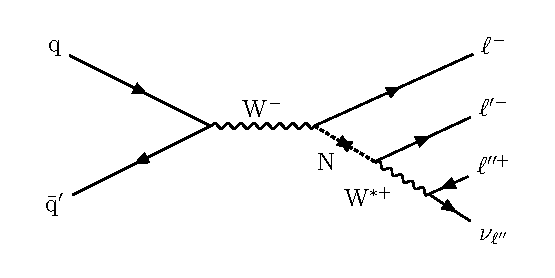
\includegraphics[width=0.44\textwidth]{Figures/c5/hnl_feyn.pdf}
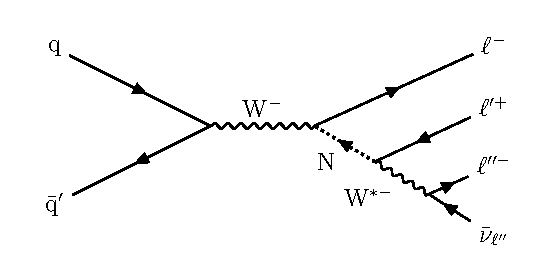
\includegraphics[width=0.44\textwidth]{Figures/c5/hnl_feyn_2.pdf}\\
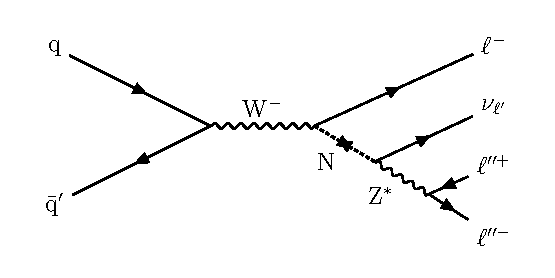
\includegraphics[width=0.44\textwidth]{Figures/c5/hnl_z_feyn.pdf}
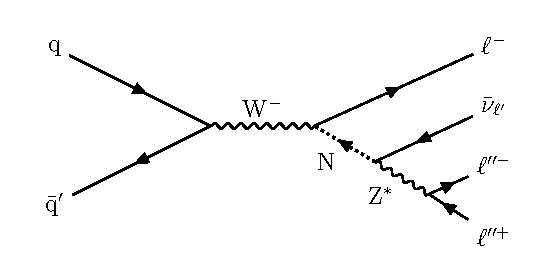
\includegraphics[width=0.44\textwidth]{Figures/c5/hnl_z_feyn_2.pdf}
\caption{Typical diagrams for the production of a HNL ($\hnl$)  at the LHC 
through its mixing with a SM neutrino, leading to a
final state with three charged leptons and a neutrino.}
\label{fig:c5hnldiagram}
\end{figure}

The final results of this analysis will be presented as sensitivity
curve as a function of both the mass and the mixing parameter, \mixpar
of the HNLs. 

\section{Analysis setup}
\subsection{Data and simulation samples}
The current analysis uses the set of \Pp collision data collected during the 2016 run at center-of-mass energy of 13\TeV corresponding to
an integrated luminosity of 35.9 \fbinv. 

A number of signal models, as described in the previous
chapter, Section~\ref{sec:c4hnlmodel}, were simulated with NLO precision in
perturbative QCD. 

The luminosity scenario has a 25 ns bunch crossing separation with an
average of about 23 pileup interactions per bunch
crossing, for details refer to Section~\ref{lhc}.

\subsection{Signal compression and trigger strategy}\label{sec:compression}
A challenging aspect of the signal under consideration is that, except
for very high masses, the \pt
spectra of the resulting leptons are in general very soft and they are
all collected in the same low \pt region; we can say that the \pt
spectra are compressed. The degree of this compression, and which
leptons are affected, depends on the mass of the produced HNL. The \pt
spectrum of the three highest \pt generator-level charged leptons is shown in figure~\ref{fig:genPt} for different HNL mass scenarios, ranging from 5 to 200 \GeV . 

\begin{figure}[h]
\noindent
\makebox[\textwidth]{
\subfloat[]{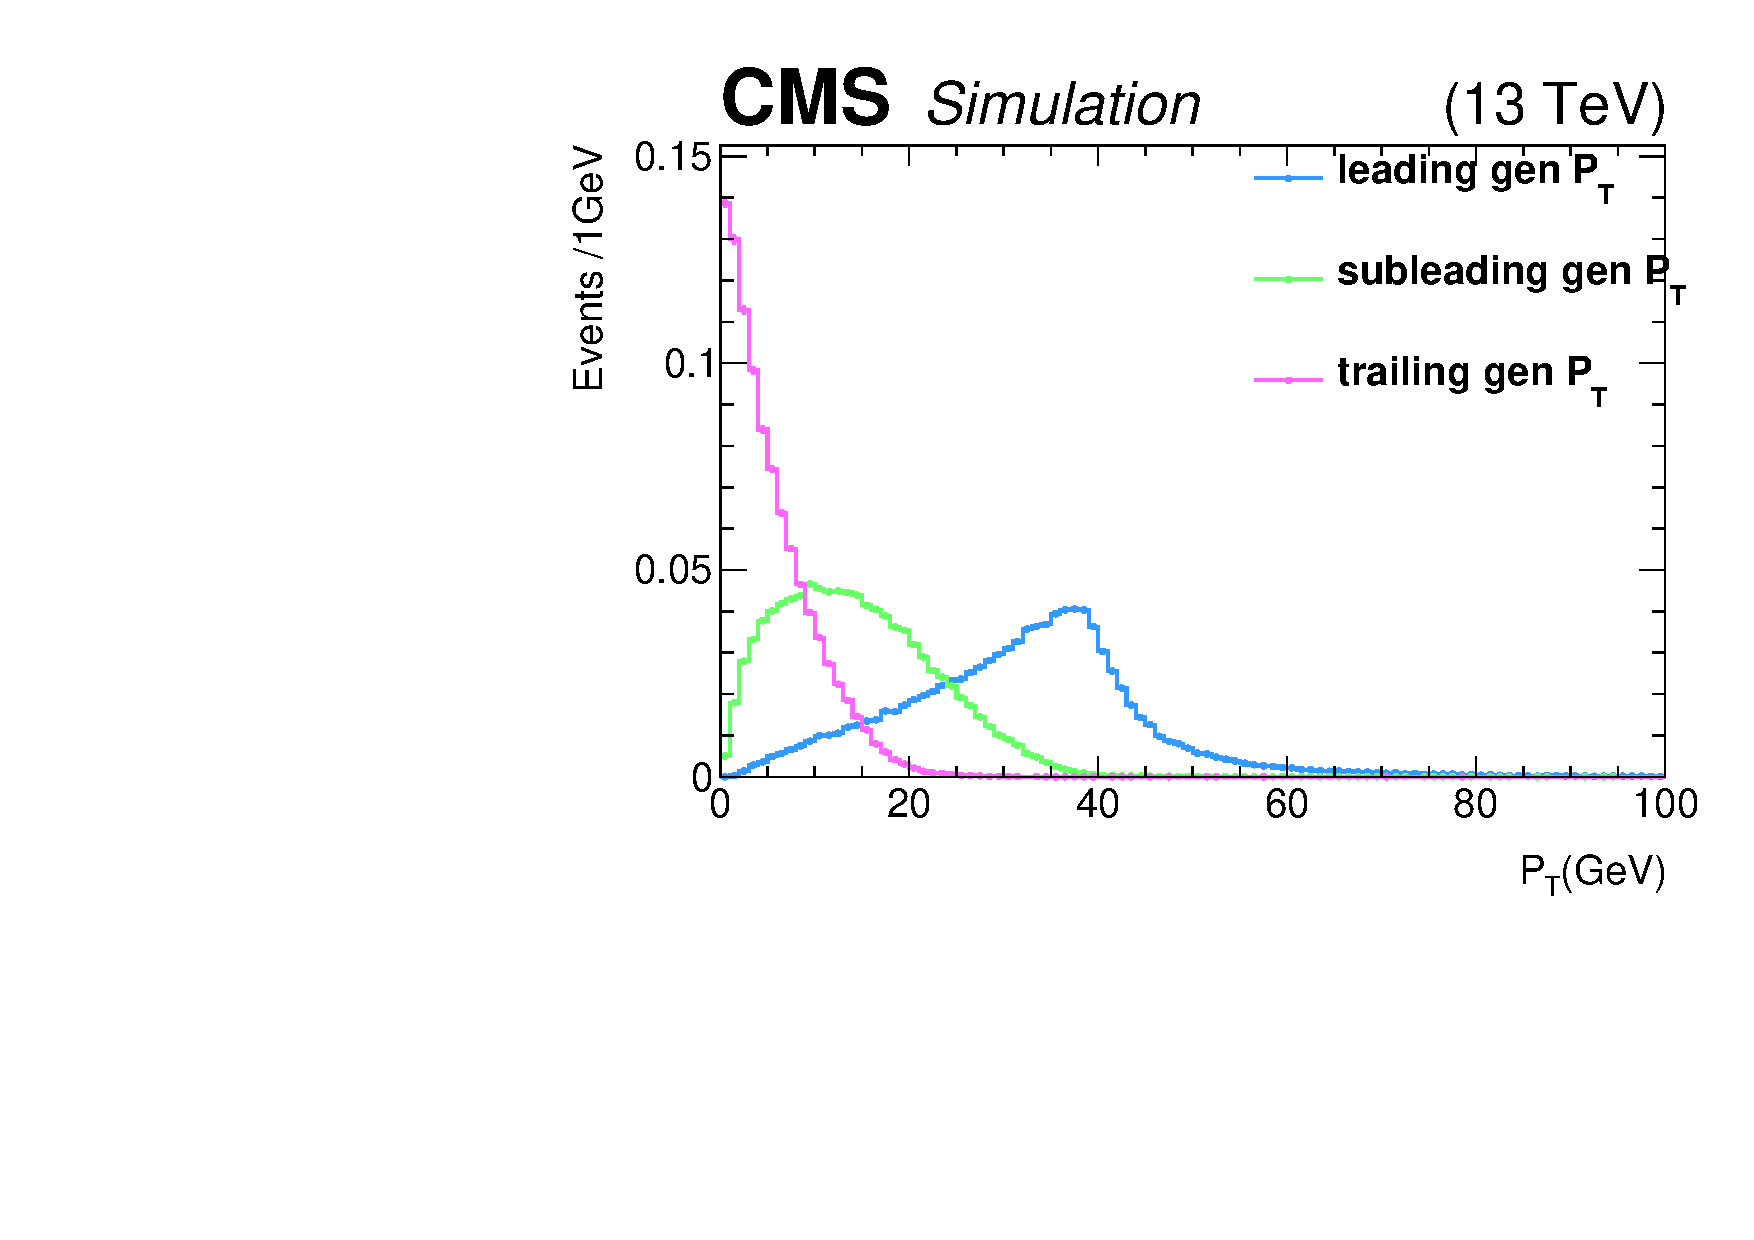
\includegraphics[width=.33\textwidth]{Figures/c5/genPt/genPtm5.pdf}}
\subfloat[]{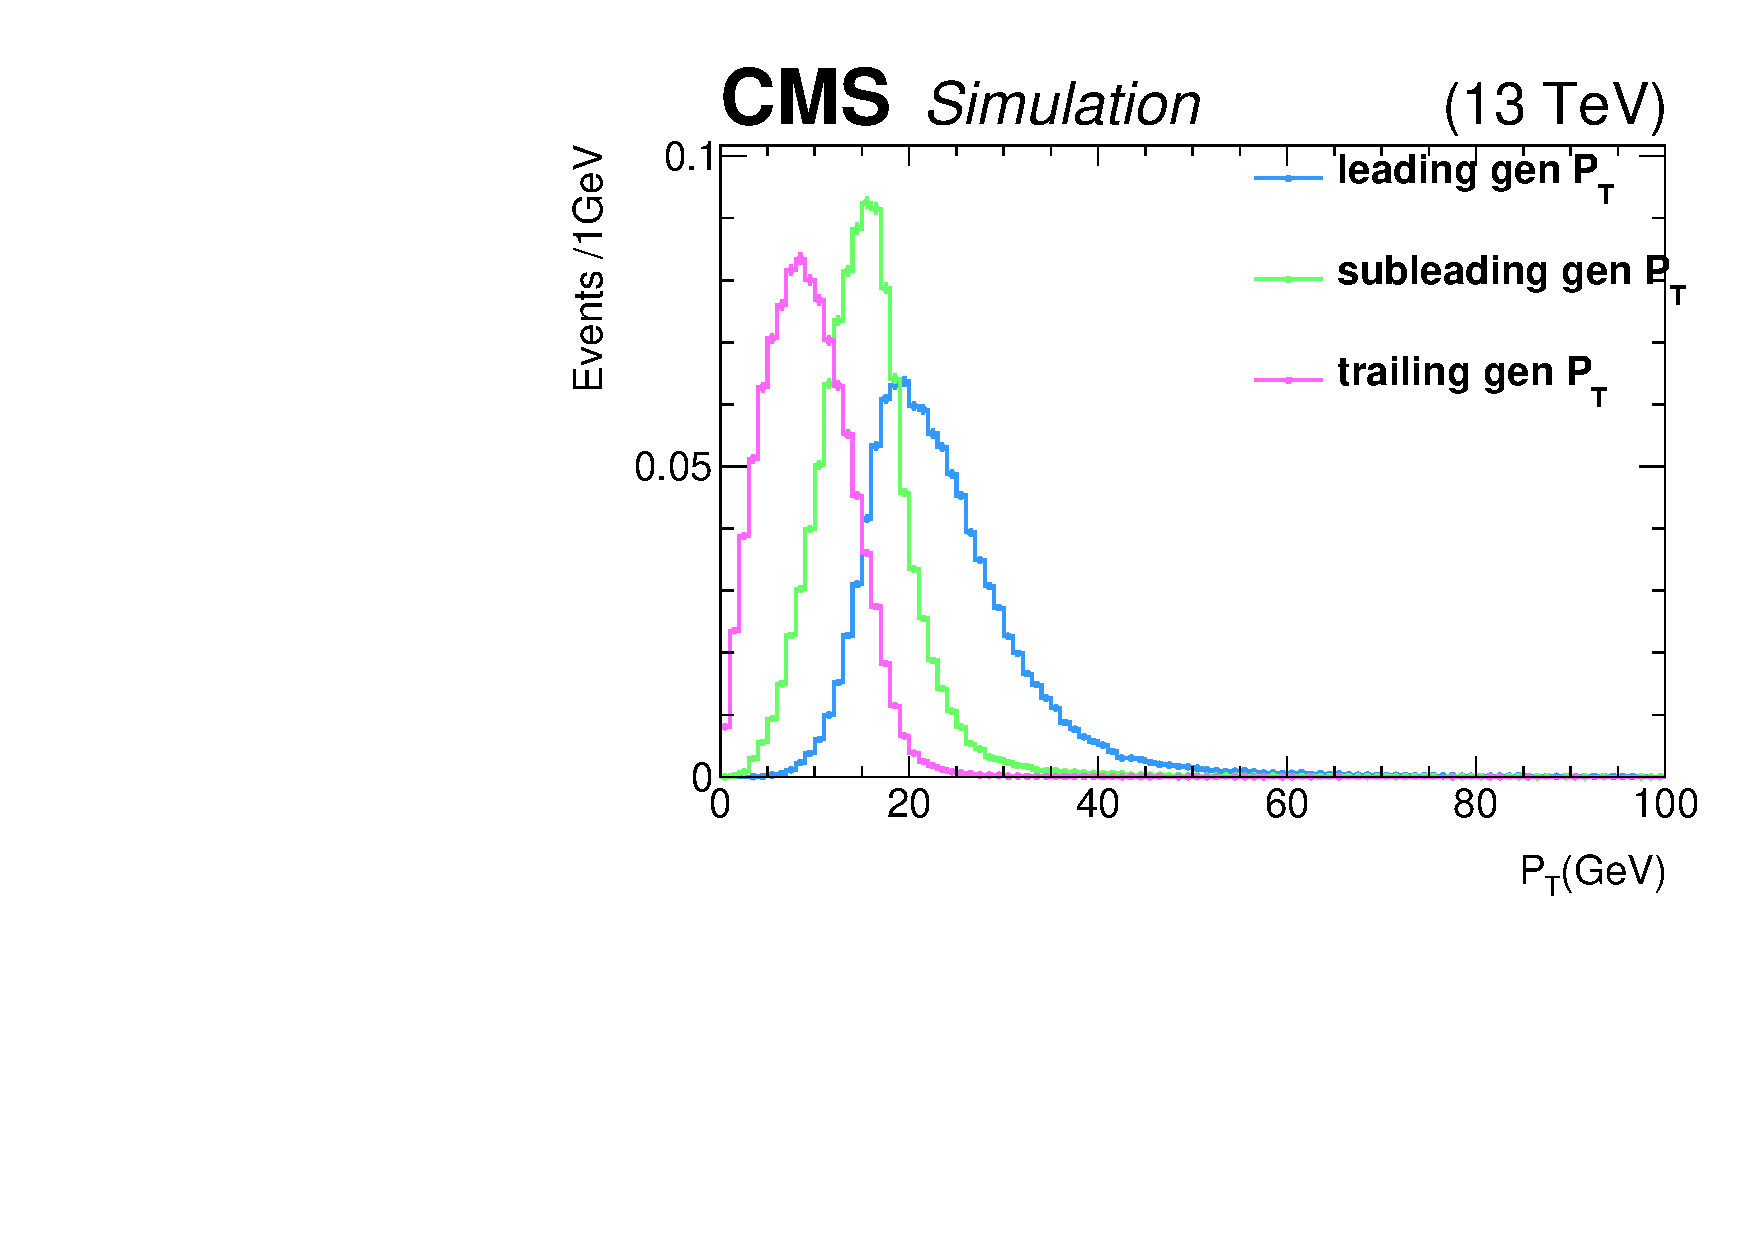
\includegraphics[width=.33\textwidth]{Figures/c5/genPt/genPtm60.pdf}}
\subfloat[]{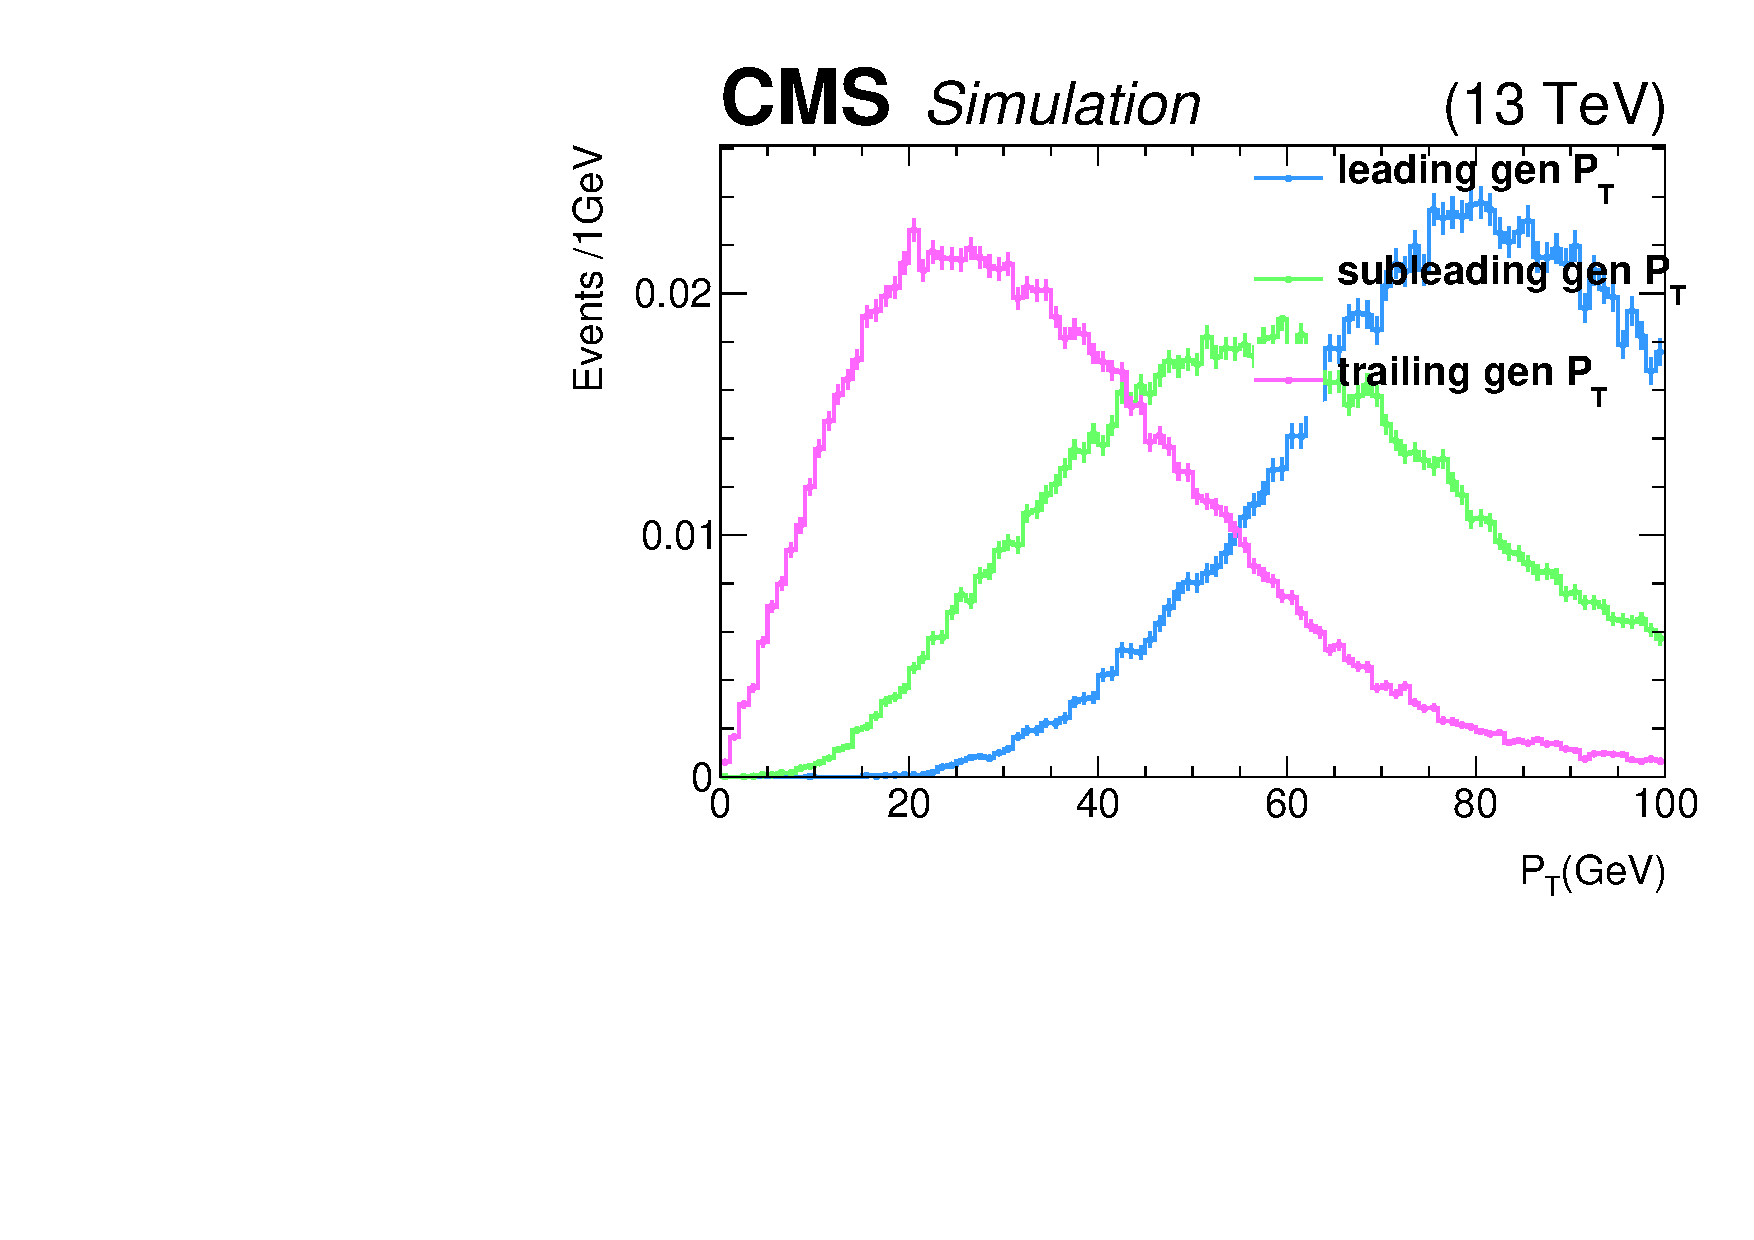
\includegraphics[width=.33\textwidth]{Figures/c5/genPt/genPtm200.pdf}}}
\caption{\pt spectrum of the three highest generator-level leptons in
  the signal simulation of several HNL masses. From top left to bottom
  right the HNL mass scenarios for which the spectrum is shown are
  5\GeV (A), 60\GeV (B), and 200\GeV (C). \willem}
\label{fig:genPt}
\end{figure}

It can be seen that for every mass scenario below the W-mass, one or
more leptons have a tendency to have very low \pt values. For low mass
samples both the trailing and sub-leading leptons are soft because of
the small mass of the decaying HNL. For HNL masses close to the mass of
the W, very little phase space is left for the emission of the lepton
in the W's decay since all of the W's mass has to go into the
production of the HNL. For high masses on the other hand, the
compression is not as pronounced even though the trailing lepton can
still be seen to prefer relatively low momenta because of the high off-shell W-boson required for production of very heavy
HNL's. Furthermore the cross section for off-shell W-boson production drops
rapidly with increasing mass, and as such the lepton with smallest \pt
also tends to have very little phase space available for its production in
very high mass scenarios.

We can clearly notice in Figure~\ref{fig:genPt} different lepton \pt spectra according to the
$M_\hnl$ and the correlation between the distributions and the $M_\PW$. For this reason the analysis
strategy has been divided in two main phase spaces:
\begin{itemize}
\setlength\itemsep{-0.2em}
\item \emph{low mass search:} soft leptons, $M_\hnl < M_\PW$;
\item \emph{high mass search:} hard leptons, $M_\hnl > M_\PW$;
\end{itemize}

\subsubsection{Trigger strategy}
Due to the low \pt spectra of the leptons in the HNL signals, designing a trigger strategy is a challenging task. 
For high HNL masses, the leading lepton \pt is generally on the efficiency plateau of the single-lepton triggers.
For low HNL masses, we need to add double- and triple-lepton triggers to obtain optimal signal efficiency.
The list of triggers used in this analysis are listed in table~\ref{table:HNL_trigger_thresholds}.


\begin{table}[h]
\centering
{\scriptsize
 \caption{Overview of the lepton \pt thresholds imposed in the analysis and the \pt regime in which each trigger path provides sensitivity.}
  \label{table:HNL_trigger_thresholds}
  \begin{tabular}{c|c|ccc|l}
   \hline
    search region                  & lepton flavors                    & \multicolumn{3}{c|}{selected \pt range (\GeV)} & sensitive trigger paths \\
                                   & $\ell^{\text{leading}} \; \ell^{\text{subleading}} \; \ell^{\text{trailing}}$ & $\pt^\text{leading}$ & $\pt^\text{subleading}$ & $\pt^\text{trailing}$ & \\
    \hline
    \multirow{12}{*}{low mass}     & $ee\mu$                           & 30--55 & $>15$    & $>5$     & $1e$ \\
                                   &                                   & 15--30 & $>15$    & $>8$     & $2e1\mu$ \\
                                   &                                   & 23--30 & 10--15    & $>8$     & $1e1\mu$ \\
                                   &                                   & 25--30 & $>15$    & 5--8      & $2e$ \\
                                   & $e\mu e$, $\mu ee$                 & 30--55 & $>15$    & $>10$    & $1e$ or $1\mu$ \\
                                   &                                   & 15--30 & $>15$    & $>15$    & $2e1\mu$ \\
                                   &                                   & 23--30 & $>10$    & 10--15    & $1e1\mu$ \\
                                   & $\mu\mu e$                        & 30--55 & $>15$    & $>10$    & $1\mu$ \\
                                   &                                   & 15--30 & $>10$    & $>10$    & $1e2\mu$ \\
                                   & $\mu e \mu$, $e\mu\mu$            & 30--55 & $>10$    & $>10$    & $1e$ or $1\mu$ \\
                                   &                                   & 15--30 & $>10$    & $>9$     & $1e2\mu$ \\
                                   &                                   & 23--30 & $>10$    & 5--9      & $1e1\mu$ \\
    \hline
    high mass                      & all flavors
                                                                       & $> 55$    & $>15$    & $>10$  & all paths \\
 \hline
  \end{tabular}
}
\end{table}

The overall approach to selecting the offline thresholds in the analysis is the following:
.


\begin{itemize}
\setlength\itemsep{-0.1em}
\item Each trigger path could select one or more leptons (refer to
  table~\ref{table:HNL_trigger_thresholds} for all the used trigger paths); furthermore for
  each lepton a specific efficiency can be individually measured, it
  will be referred as lepton-specific efficiency. Then data/MC scale
  factors (SF) are calculated for each used
  lepton-specific trigger and determine values where these SFs are
  constant. 
 Typical SF values are 98\% for a muon-specific and 99\% for an electron-specific. 
\item determine total efficiency of trigger combinations (not anymore
  lepton-specific) in MC simulation, and choose \pt thresholds leading to the highest overall efficiency and being not lower than the values determined in the first step;
\item check the overall data/MC SF in an orthogonal and unbiased dataset which was
  selected by triggering on \ptmiss or on the hadronic activity of the event;
\item determine systematics from the SF values obtained in the first step and validate its choice in the previous step: 
\begin{itemize}
\setlength\itemsep{-0.2em}
\item use 5\% systematics for events with leading lepton $\pt < 30$\GeV (max. SF value for $\Pe\Pe\mu$ and $\Pe\mu\mu$ case),
\item and 2\% for events with leading lepton $\pt > 30$\GeV (max. SF value of a muon leg).
\end{itemize}
\item require trigger information in MC samples when deriving the yields, but not apply any additional correction.
\end{itemize}


\iffalse
We use the tag-and-probe method to measure the lepton-specific efficiencies. The efficiency is 
defined as the ratio of selected events where the probe matches the lepton-specific in question ($\Delta R<0.4$) over 
the total number of selected events. Events entering the denominator in data are taken from the 
SingleElectron (SingleMuon) dataset and must fire an unprescaled
single lepton trigger with \pt threshold > 27\GeV (> 24\GeV).
Requiring the tag and the probe to both pass the offline lepton selection reduces the contamination 
from fakes at sub-percent level. We therefore do not perform any background subtraction using a fit to 
the \PZ peak. This choice presents the advantage that the measurement in channels purely dominated by the 
Drell-Yan process ($\Pe\Pe$ and $\mu\mu$) can be compared to a channel where the contribution from \ttbar 
becomes dominant at high lepton $\pt$ ($\Pe\mu$).
In order to estimate the uncertainty on the trigger efficiency for the OR combination of single, double and trilepton triggers,
we select trilepton events according to the baseline selection criteria described in Section~\ref{sec:object}.
The trigger efficiency is then measured as a function of the trailing
lepton \pt in both the unbiased \verb!MET! dataset, a high-statistics $\PW\PZ$ MC sample and a HNL samples. 
The applied baseline selection criteria
ensures we are on the efficiency plateau, see Figure~\ref{fig:3l1l1lEff}, and reasonable data/MC agreement is observed 
as statistical uncertainties of the samples allow to judge.}
\fi

The overall $1\ell+2\ell+3\ell$ trigger efficiency was measured in WZ MC samples 
after selecting 3 leptons with relevant flavor combinations which pass
the offline analysis identification selection. The efficiency is typically close to 100\%
and always above 92\%, for events with leading lepton \pt $> 30$\GeV. For
events in which the leading lepton \pt is $< 30$\GeV, the efficiency
falls down reaching the value of 70\% in the worst case scenario.
Hence we assign a 5\% uncertainty
on the trigger efficiency for leading lepton $\pt < 30$\GeV
$\;$ and for $\pt > 30$\GeV we assigned a 2\%
uncertainty. 

\iffalse
\begin{figure}[h]
\noindent
\makebox[\textwidth]{
  \subfloat[{\tiny$3\Pe$, $\pt^\text{lead} > 55\GeV$}]{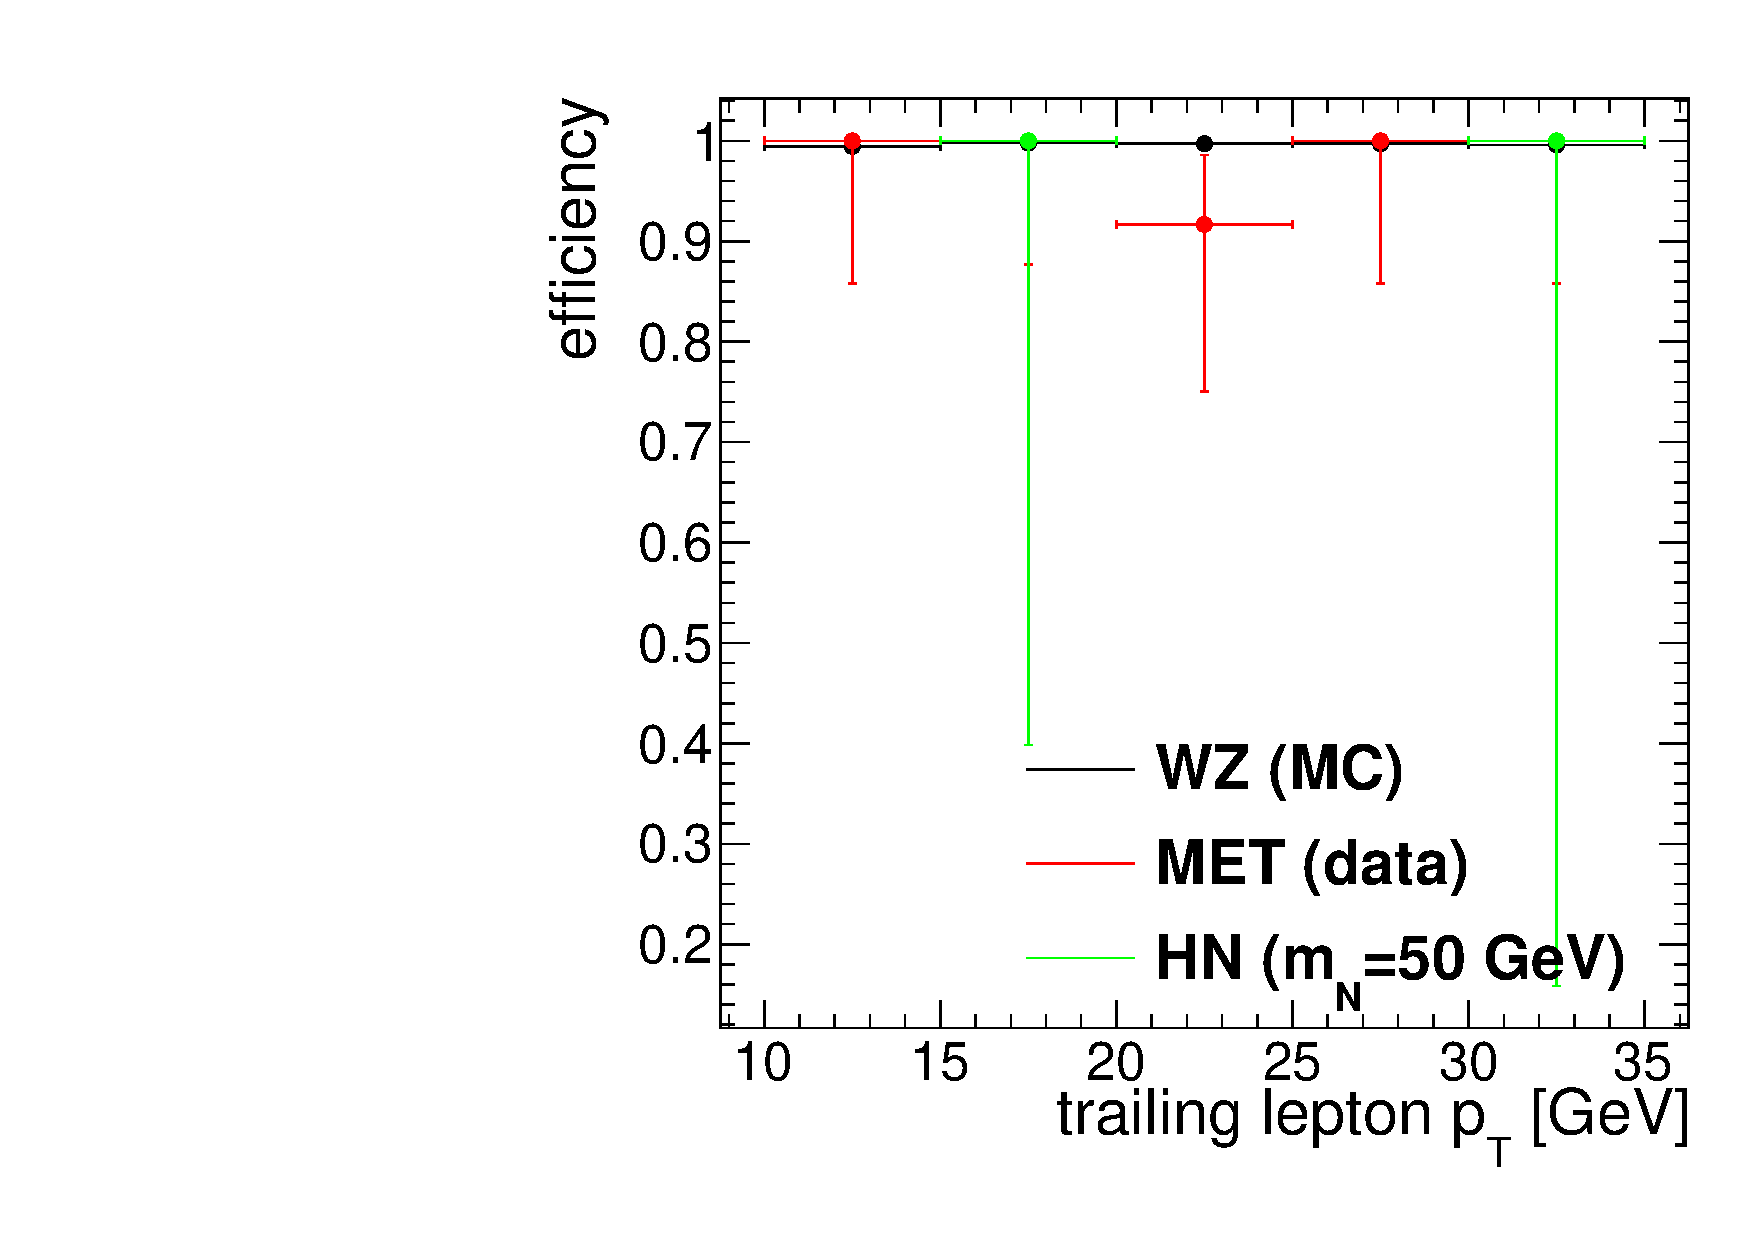
\includegraphics[width=0.34\textwidth]{Figures/c5/trigger/vsTrailingPt/eee_pt55to1000.pdf}}
  \subfloat[{\tiny$3\mu$, $\pt^\text{lead} > 55\GeV$}]{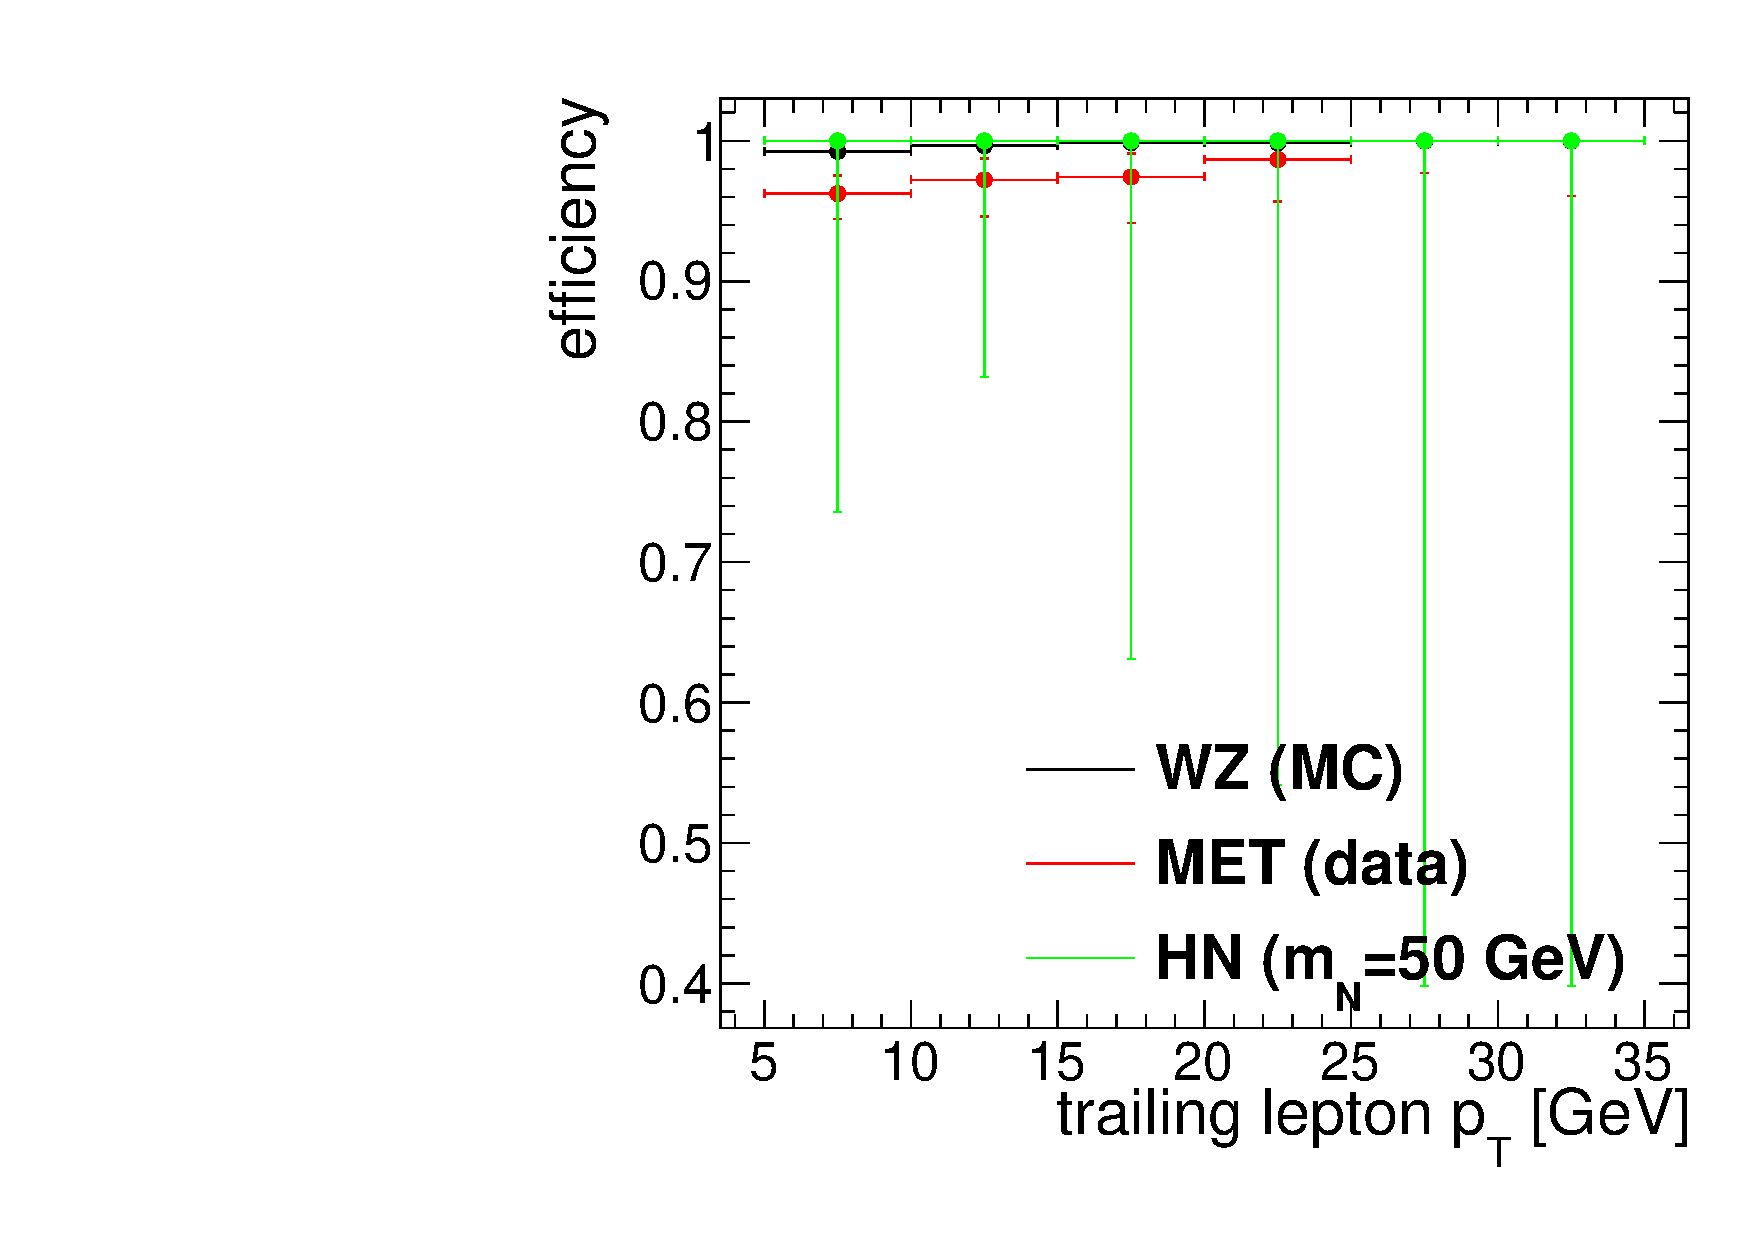
\includegraphics[width=0.34\textwidth]{Figures/c5/trigger/vsTrailingPt/mumumu_pt55to1000.pdf}} 
  \subfloat[{\tiny$2\Pe1\mu$, $\pt^\text{lead} [15,30] $}]{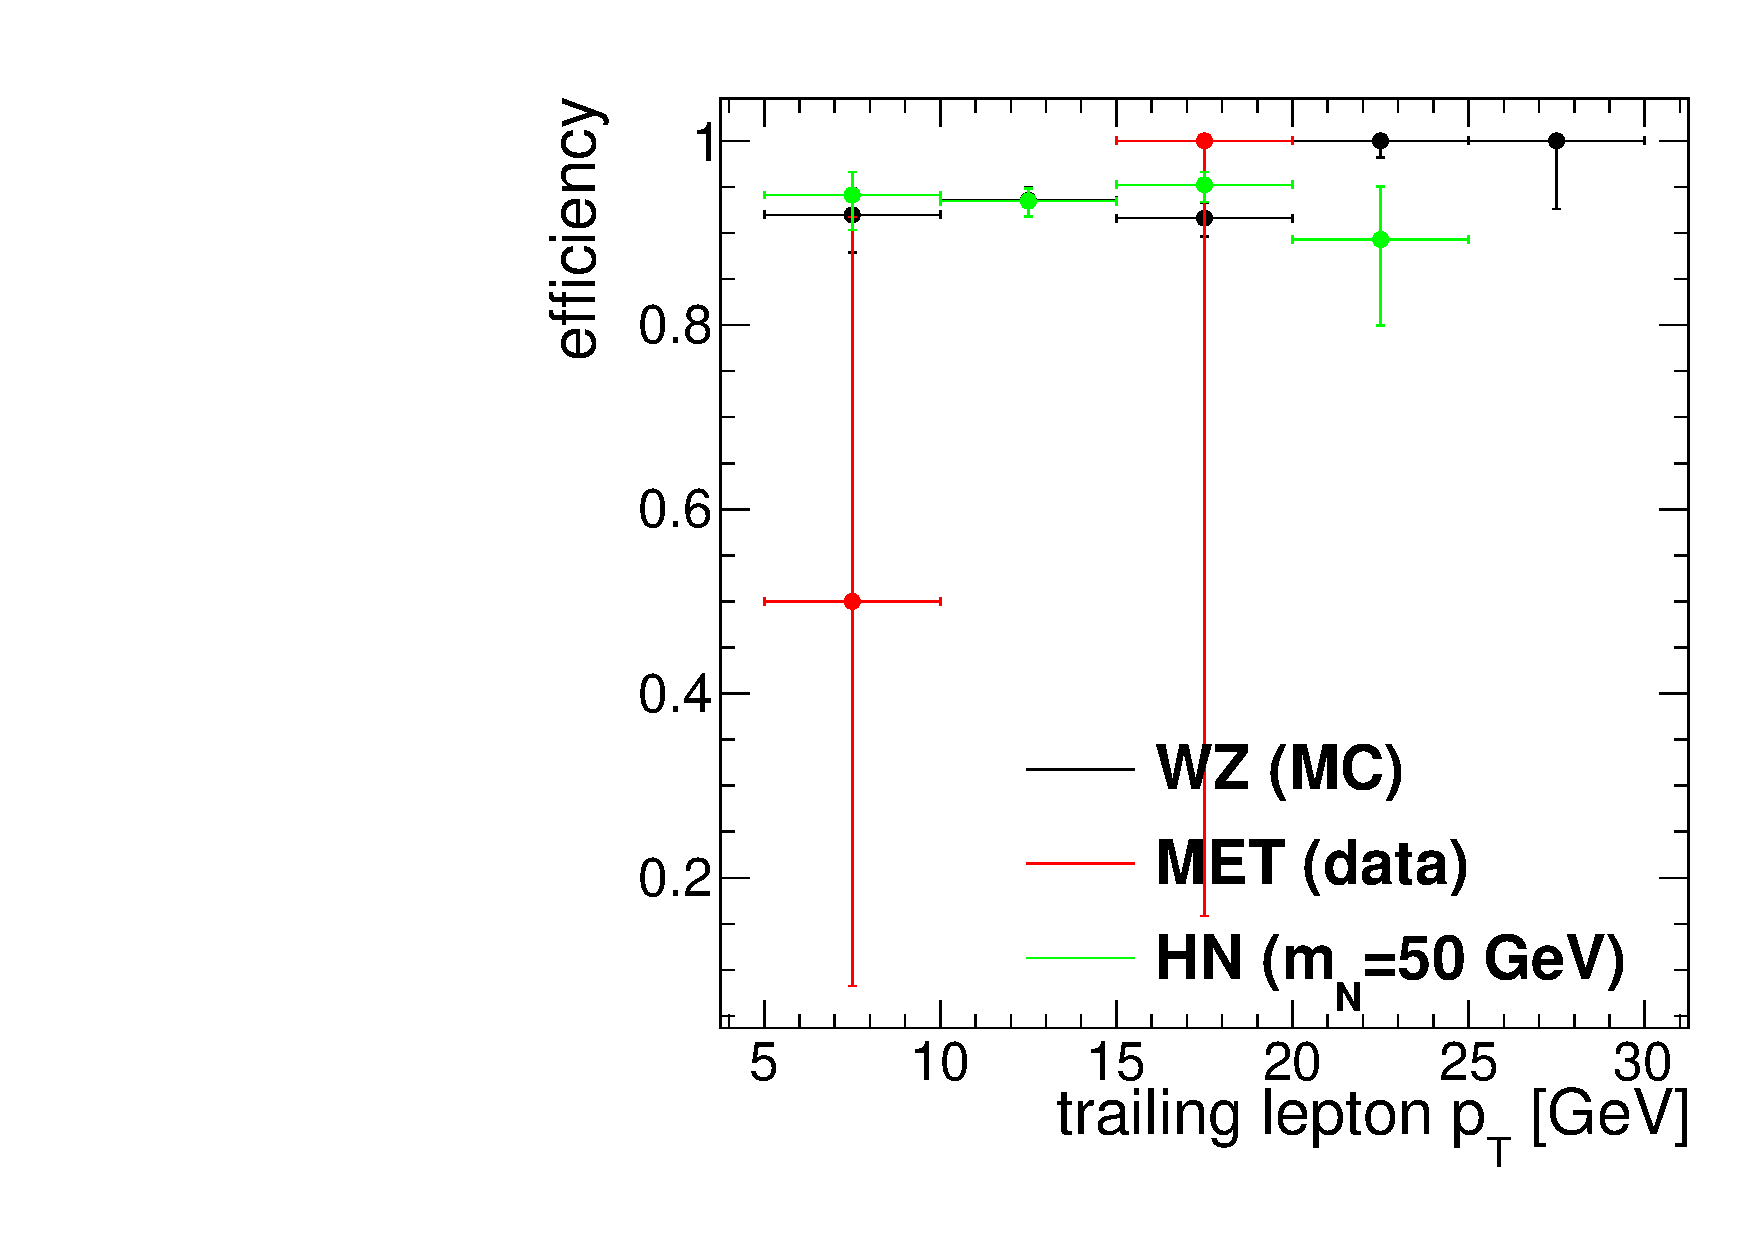
\includegraphics[width=0.34\textwidth]{Figures/c5/trigger/vsTrailingPt/eemu_pt0to30.pdf}}}\\
  \noindent
\makebox[\textwidth]{
  \subfloat[{\tiny$2\Pe1\mu$, $\pt^\text{lead} [30,55] $}]{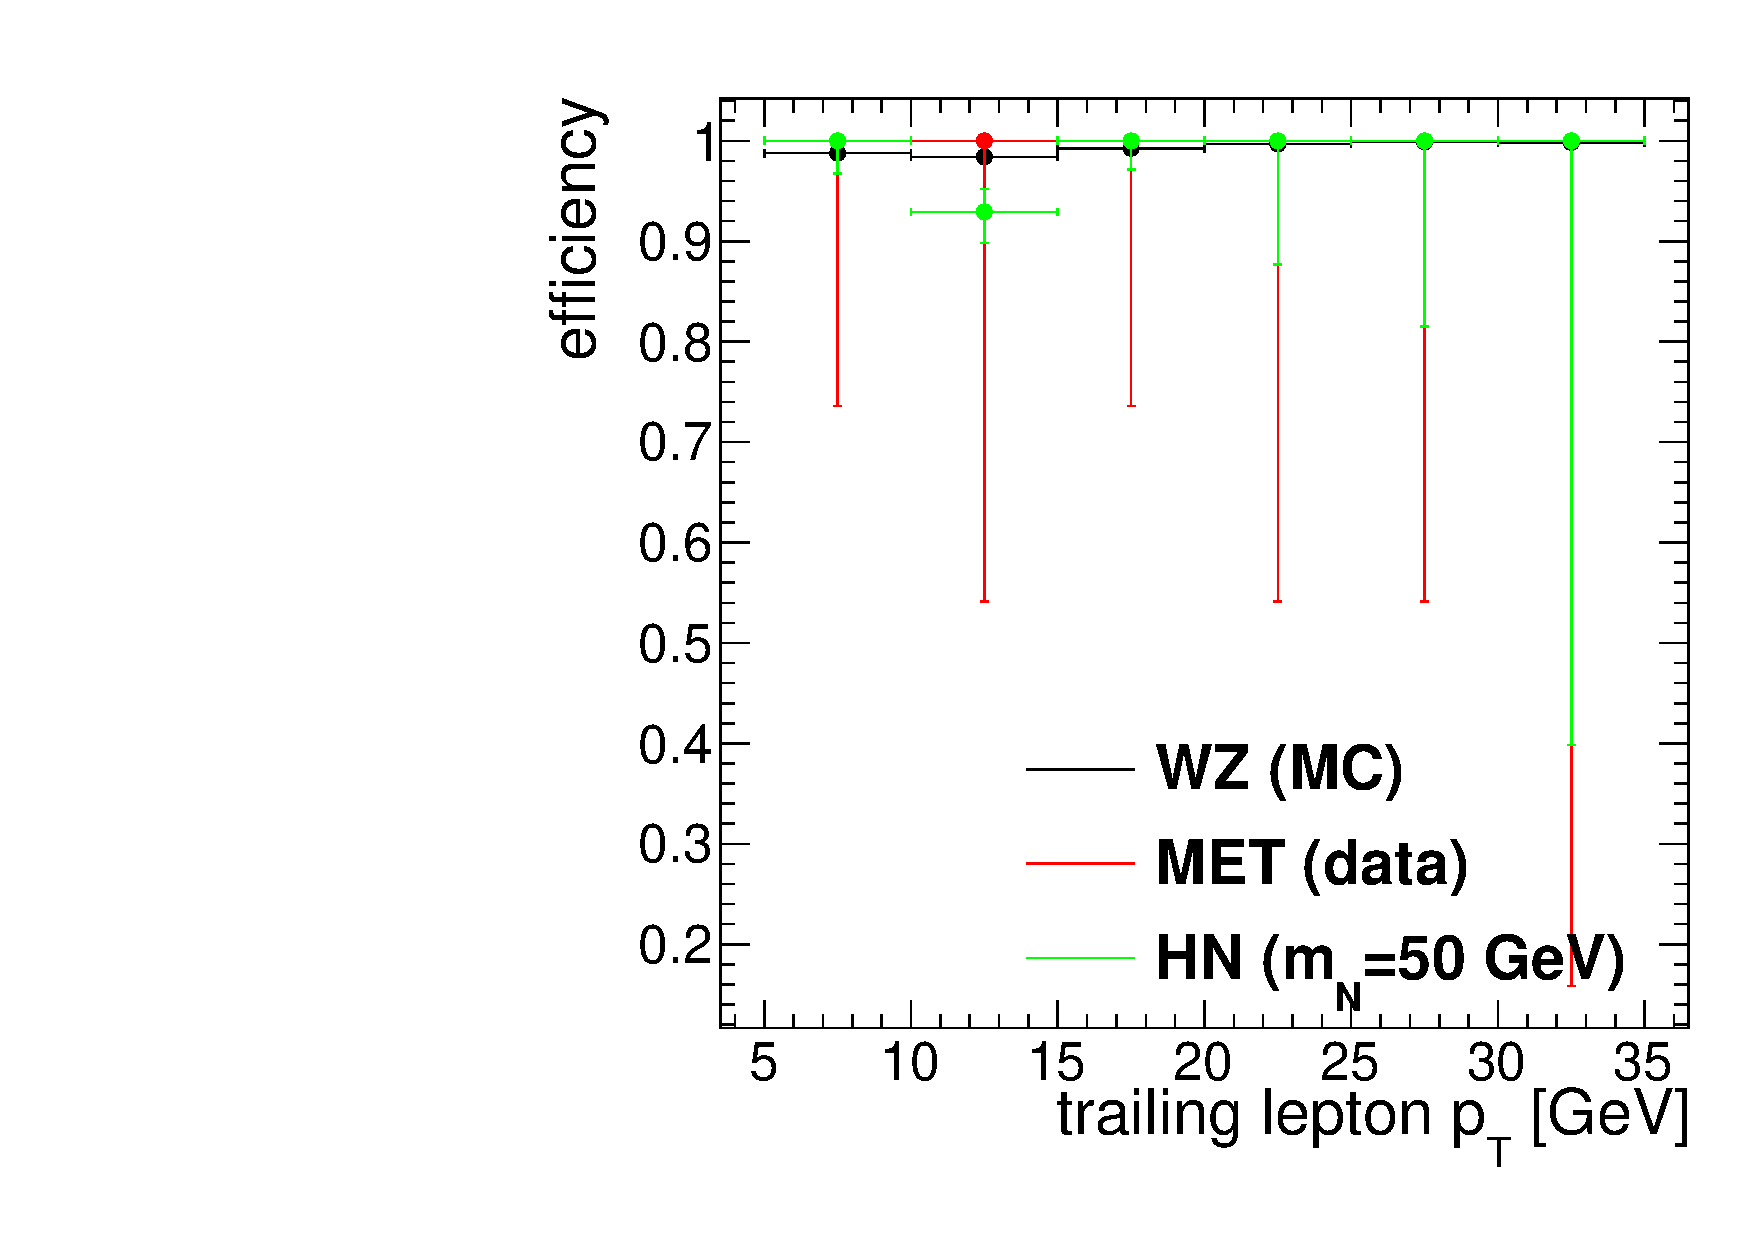
\includegraphics[width=0.34\textwidth]{Figures/c5/trigger/vsTrailingPt/eemu_pt30to55.pdf}} 
  \subfloat[{\tiny$1\Pe2\mu$, $\pt^\text{lead} [15,30] $}]{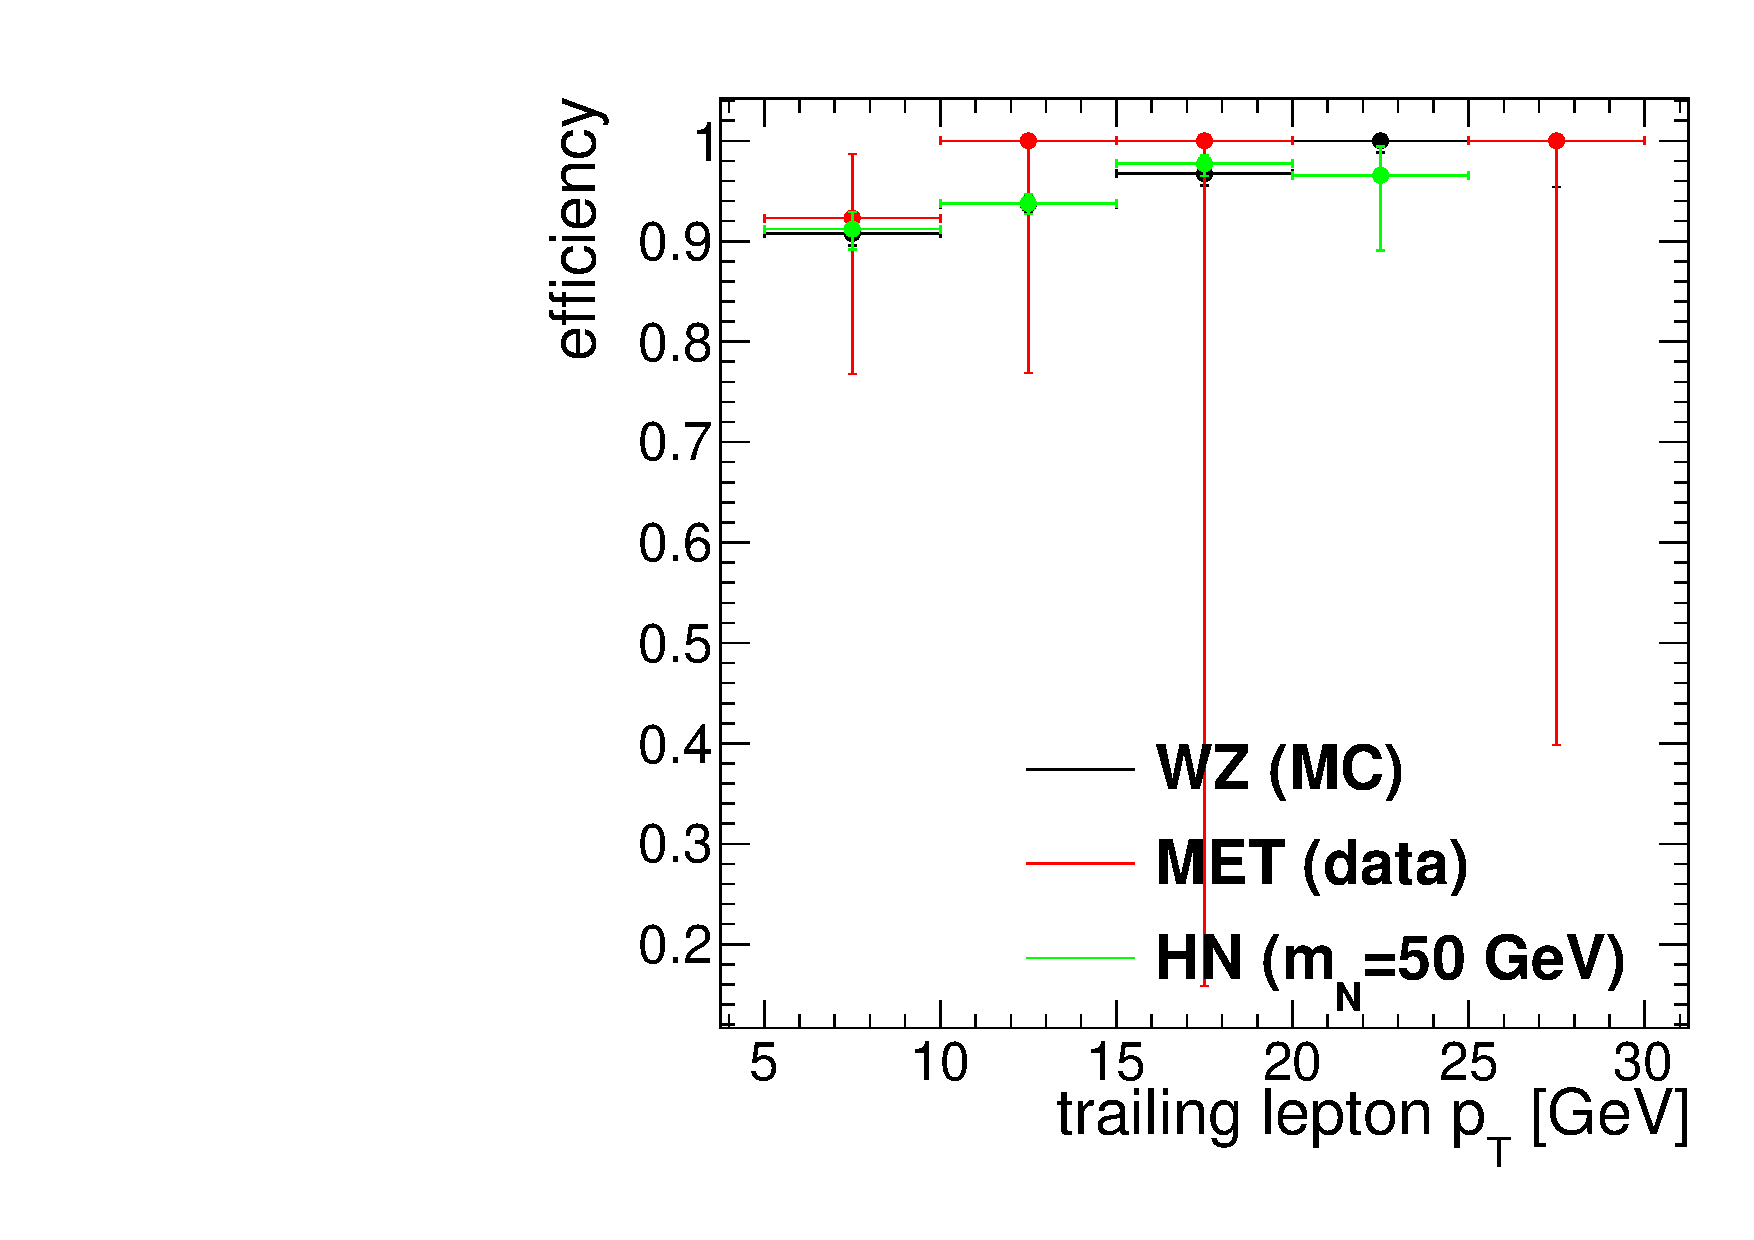
\includegraphics[width=0.34\textwidth]{Figures/c5/trigger/vsTrailingPt/emumu_pt0to30.pdf}}
  \subfloat[{\tiny$1\Pe2\mu$, $\pt^\text{lead} [30,55] $}]{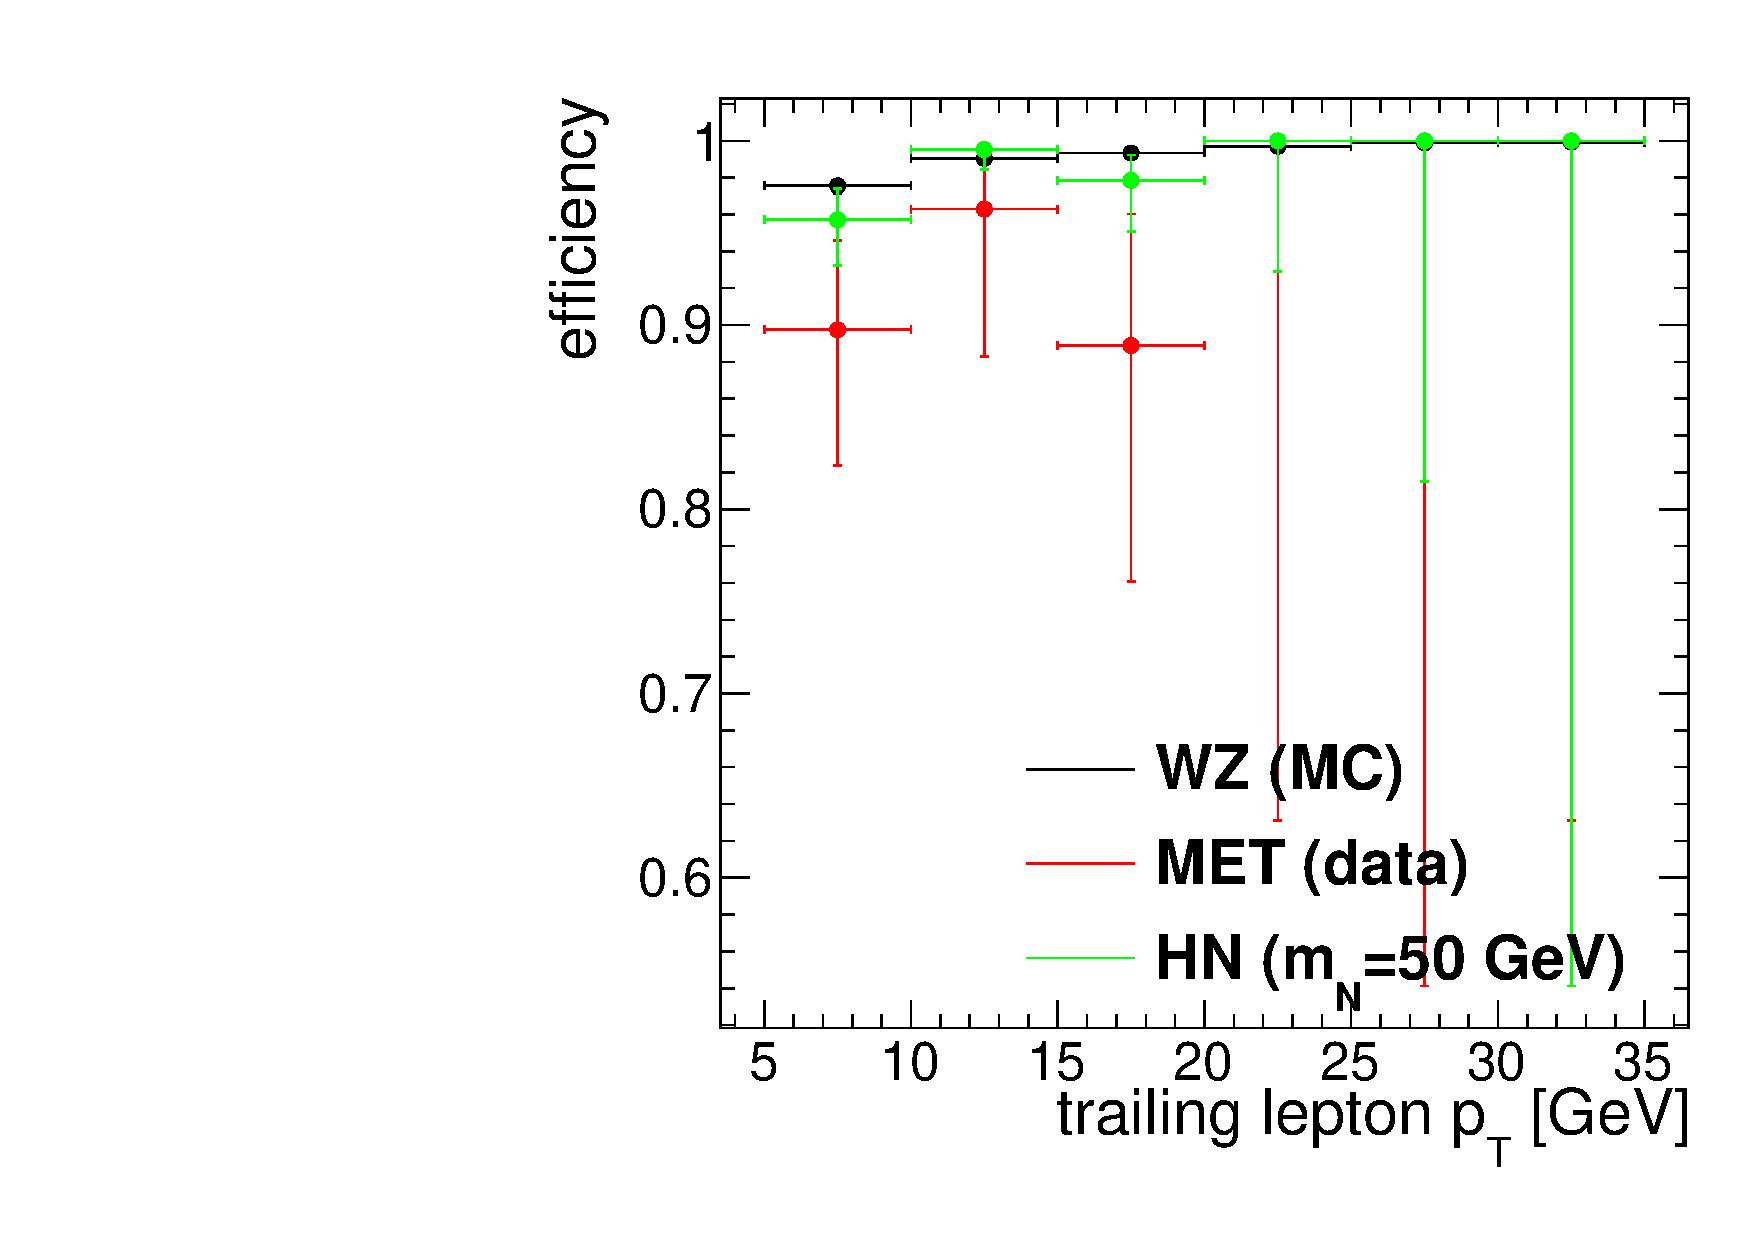
\includegraphics[width=0.34\textwidth]{Figures/c5/trigger/vsTrailingPt/emumu_pt30to55.pdf}}}\\
  \caption{Efficiencies for the OR combination of single, double and trilepton triggers, in trilepton events as a function
  of the trailing lepton \pt.}
  \label{fig:3l1l1lEff}
\end{figure}
\fi

\subsection{Object selection}\label{sec:object}
For the rigorous explanation of the single object reconstruction in
CMS see Chapter~\ref{Chapter2_5}, section~\ref{sec:reconstruction}.

\subsubsection{Leptons}
The base objects of this analysis are electrons and muons. Both
electrons and muons have three selection working points, called
\textsc{loose}, \textsc{fakeable object} (\textsc{FO}) and \textsc{tight}~\footnote{
N.B. these working points do not necessarily coincide with the ones
defined in Sections~\ref{sec:c2muonselection}
and~\ref{sec:c2keleid}. For these latter the italic style is used.} which
are specifically delineated for this analysis. The \lo working point
is used when cleaning electrons from overlap with muons, to be
specific, electrons are not considered for selection if they fall
within a cone of $\Delta \mathrm{R} = 0.05$ around a \lo muon. The
\fo working point is slightly tighter than the \lo one, and is
extensively used for the estimation of the background due to
nonprompt and fake leptons as described further in this text. The
ideal feature of a typical \fo working point is that after applying it
the probability that a selected nonprompt lepton also passes the
\ti working point should be independent
 of the flavor of its origin parton.
 This property will prove essential for the nonprompt lepton background estimation as further specified. The full definitions of each selection working point, for respectively muons and electrons are shown in tables ~\ref{tab:muonIDs} and \ref{tab:eleIDs}.

Signal leptons are required to be isolated (refer to
Section~\ref{sec:c2iso}) from any hadronic activity
in the event. \lo and \fo leptons are required to have $\Irel < 0.6$. 
\ti leptons must satisfy $\Irel < 0.1$.

\begin{table}[h!]
\centering
{\scriptsize
\caption{All the variables used in the table are introduced in
  Chapter~\ref{Chapter2_5} in Sections~\ref{sec:reconstruction},~\ref{sec:c2muonselection}
 and~\ref{sec:c2variables}.
Requirements to pass each definition of the muon selection.}
\label{tab:muonIDs}
\begin{tabular}{c|c|c|c}
\hline
\bf{Selection criteria} & \lo & \fo & \ti \\
\hline
$|\eta| < 2.4$ & \checkmark & \checkmark & \checkmark \\
$\pt$ & $>5$ & $>5$ & $>5$\\
$|d_{xy}| < 0.05$ (cm) & \checkmark & \checkmark & \checkmark \\
$|d_z| < 0.1$ (cm) & \checkmark & \checkmark & \checkmark \\
$\text{SIP}_{3D} < 4$ & -- & \checkmark & \checkmark \\
$\Irel$ & $<0.6$ & $<0.6$ & $<0.1$ \\
is PF Muon & \checkmark & \checkmark & \checkmark \\
is Global or Tracker Muon & \checkmark & \checkmark & \checkmark \\
is \textit{Medium} Muon & -- & \checkmark & \checkmark \\
\hline
\end{tabular}
}
\end{table}


\begin{table}[h!]
\centering
{\scriptsize
\caption{All the variables used in the table are introduced in
  Chapter~\ref{Chapter2_5} in Sections~\ref{sec:reconstruction},~\ref{sec:c2keleid}
 and~\ref{sec:c2variables}.}
\label{tab:eleIDs}
\resizebox{1.0\linewidth}{!}{
\begin{tabular}{c|c|c|c}
\hline
\bf{Selection criteria} & \lo & \fo & \ti \\
\hline
$|\eta| < 2.5$ & \checkmark & \checkmark & \checkmark \\
$\pt$ & $>10$ & $>10$ & $>10$ \\
$|d_{xy}| < 0.05$ (cm) & \checkmark & \checkmark & \checkmark \\
$|d_z| < 0.1$ (cm) & \checkmark & \checkmark & \checkmark \\
$\text{SIP}_{3D} < 4$ & -- & \checkmark & \checkmark \\
\Irel & $<0.6$ & $<0.6$ & $<0.1$ \\
MVA ID (\pt $<$ 15 $\mathrm{GeV}$)& -- & $> (-0.02, -0.52, -0.52)$ & $> (0.77, 0.56, 0.48)$\\
MVA ID (\pt $>$ 25 $\mathrm{GeV}$)& -- & $> (-0.02, -0.52, -0.52)$ & $> (0.52, 0.11, -0.01)$\\
$\sigma_{i\eta i\eta} <(0.011,0.011,0.030)$ & -- & \checkmark & \checkmark \\
H/E $< (0.10,0.10,0.07)$ &  -- &  \checkmark & \checkmark \\
$\Delta\eta_{\textrm in} < (0.01, 0.01, 0.008)$ & -- & \checkmark & \checkmark \\
$\Delta\phi_{\textrm in} < (0.04, 0.04, 0.07)$ & -- & \checkmark & \checkmark \\
$-0.05 < 1/E-1/p < (0.010,0.010,0.005)$ & -- & \checkmark & \checkmark \\
conversion rejection & \checkmark & \checkmark & \checkmark \\
Number of missing hits & $<2$ & $== 0$ & $== 0$ \\
\hline
\end{tabular}}
}
\end{table}

A notable difference between the muon and electron selection criteria
are the \pt thresholds that are being used. Considering the earlier
discussion on the compressed \pt spectra of the low HNL mass scenario, it is
clear that we want to apply \pt thresholds as low as feasible in order
to gain the maximum signal efficiency. So ideally we would want low
\pt thresholds on both muons and electrons, but for low mass search the triggers are a
limiting factor in how low we can realistically go. The higher
electron trigger thresholds make going lower than 10\GeV $\:$in electron \pt unfeasible, even though our trigger strategy is
optimized for maximum efficiency and thresholds as low as possible, as
described in the previous section. The relatively high \pt thresholds forced upon us by the available
triggers leave us with relatively low signal efficiencies, as the
often very soft trailing, and subleading signal leptons do not manage
to pass the thresholds of the baseline object selection.
 Aside from this, harsher \pt thresholds of 15 and 10\GeV $\:$are applied
 to the leading and subleading leptons in order to pass the employed
 triggers.

\section{Analysis strategy}\label{sec:analisi}
All events entering the signal regions are required to have three light leptons passing the \ti requirements as described in the section above (~\ref{sec:object}).
The events with three leptons of the same sign are not retained in the analysis. 
Events with three leptons in which one or several leptons fail the \ti
criteria, but pass the \fo selection entered the sideband region to estimate the nonprompt lepton background. The presence of a fourth \fo lepton was vetoed in order to suppress the contribution of processes yielding four leptons such as ZZ, while having only a sub-percent effect on the predicted signal yields.

Events in which a jet with \pt > 25 GeV is found, passing the loose working point of the CSV b-tagging algorithm, are rejected in order to substantially decrease the background from the \ttbar process. 

The baseline \pt cuts applied in the analysis are driven by the
trigger thresholds of the available triggers as described in
Table~\ref{table:HNL_trigger_thresholds}.

Aside from kinematic criteria, the events
are categorized according to the sign and flavor of the three
leptons; events with a OSSF (Opposite Sign Same Flavor) pair and
events without an OSSF pair. This categorization helps to discriminate between
different backgrounds and it consistently reduces the background yields
from SM processes.

As described in Section~\ref{sec:compression}, the analysis
strategy is spilt into two main phase spaces, the \emph{low mass search} ($M_\hnl <
M_\PW$) and the \emph{high mass search} ($M_\hnl > M_\PW$).

\subsection{Low mass search}

As the name suggest the low mass region focuses on
the search for HNLs of low mass, in particular those below the mass
of the W boson. These low mass HNL events are characterized by
relatively low values for \ptmiss  and for the trilepton invariant mass
\mlll. Thus, upper bounds are applied on \ptmiss  and \mlll , namely:
\ptmiss < 75\GeV and \mlll < 80\GeV. The latter requirement contributes to 
suppress the background from asymmetric external- and
internal conversions (detailed explanation of this background
contribution is given is Section~\ref{sec:conversion}). In such events, a lepton might radiate a real or
virtual photon converting into a lepton pair where one lepton takes
away most of the photon's energy, and the second lepton ends up
failing basic selection requirements. A large contribution of such
events is expected from Z + $\gamma$ process, mainly having \mlll
values close to the Z boson mass.
The \ptmiss threshold is applied since almost all low mass HNL production
events fall below this value, whereas several major backgrounds such
as \ttbar and $WZ$ often have larger \ptmiss  values.

The low mass HNL search is split into two distinct categories. Events
are categorized according to the \pt of the leading lepton as
anticipated earlier. A first category consists of events with leading
lepton \pt values between 30 and 55\GeV. This category mainly targets
HNL scenarios in which the difference between the W mass and the HNL
is large, in other words very low HNL masses, in which the leading
lepton is expected to be hard. The second category is characterized by
leading lepton \pt values below 30\GeV, and mainly used for inquiring
the existence of HNLs with masses close to that of the W boson. In
such cases the limited phase space available for the production of the
charged lepton in the W decay, and the other in the HNL decay leads to
three relatively soft leptons.
Dedicated studies were performed in order to select the optimal value
of the upper \pt cut on the leading lepton \pt.
The implementation of this upper \pt cut can be seen to help reduce the background significantly while only minimally affecting the signal efficiency.

The low mass category of this analysis only considers events without
an OSSF pair due to the massive contribution of Drell-Yan + jets, asymmetric
conversion and $WZ$ backgrounds in events with an OSSF pair.
Though it is combinatorially more likely for the signal to contain an
OSSF pair, the background is multiple orders of magnitude larger for
such events,
and the sensitivity was negligible compared to events without an OSSF
pair.
Attempts were made to define search regions for such events, which
ended up being roughly two orders of magnitude less sensitive than
those without an OSSF pair. Thus, these events are not further
considered for low mass search.

The summary of the \emph{low mass} search event selection is listed in Table~\ref{tab:lowMEventSelectio}.

\begin{table}[h]
  \centering
  \caption{\label{tab:lowMEventSelectio} Baseline selection requirements
    applied to all data sets for the \emph{low mass} search.}
  \begin{tabular}{l|l}
    \hline
    Variable     & Requirement       \\
    \hline
    \hline
     N. \PQb & = 0              \\
    4th $\ell$ veto & \checkmark       \\
    $\pt^{\text{leading}}$ & < 55 \GeV\\
     \mlll & < 80\GeV\\
    \ptmiss &  < 75\GeV\\
    \hline
    \hline
  \end{tabular}
\end{table}

In the selected events without an OSSF pair, the best discrimination
between the signal and the background came from
the minimal invariant mass, \mmin, out of all possible pairs of
opposite sign leptons in the event. 
The distribution of this variable is shown for the signal and the
background in Figure~\ref{fig:MminMos} (left) before the low/mass
categorization. In Figure~\ref{fig:MminMos} (middle/right) the \mmin distribution is shown for the signal and the
background for both the low and high leading
\pt categories of the low mass search.

\begin{figure}[h]
\noindent
\makebox[\textwidth]{  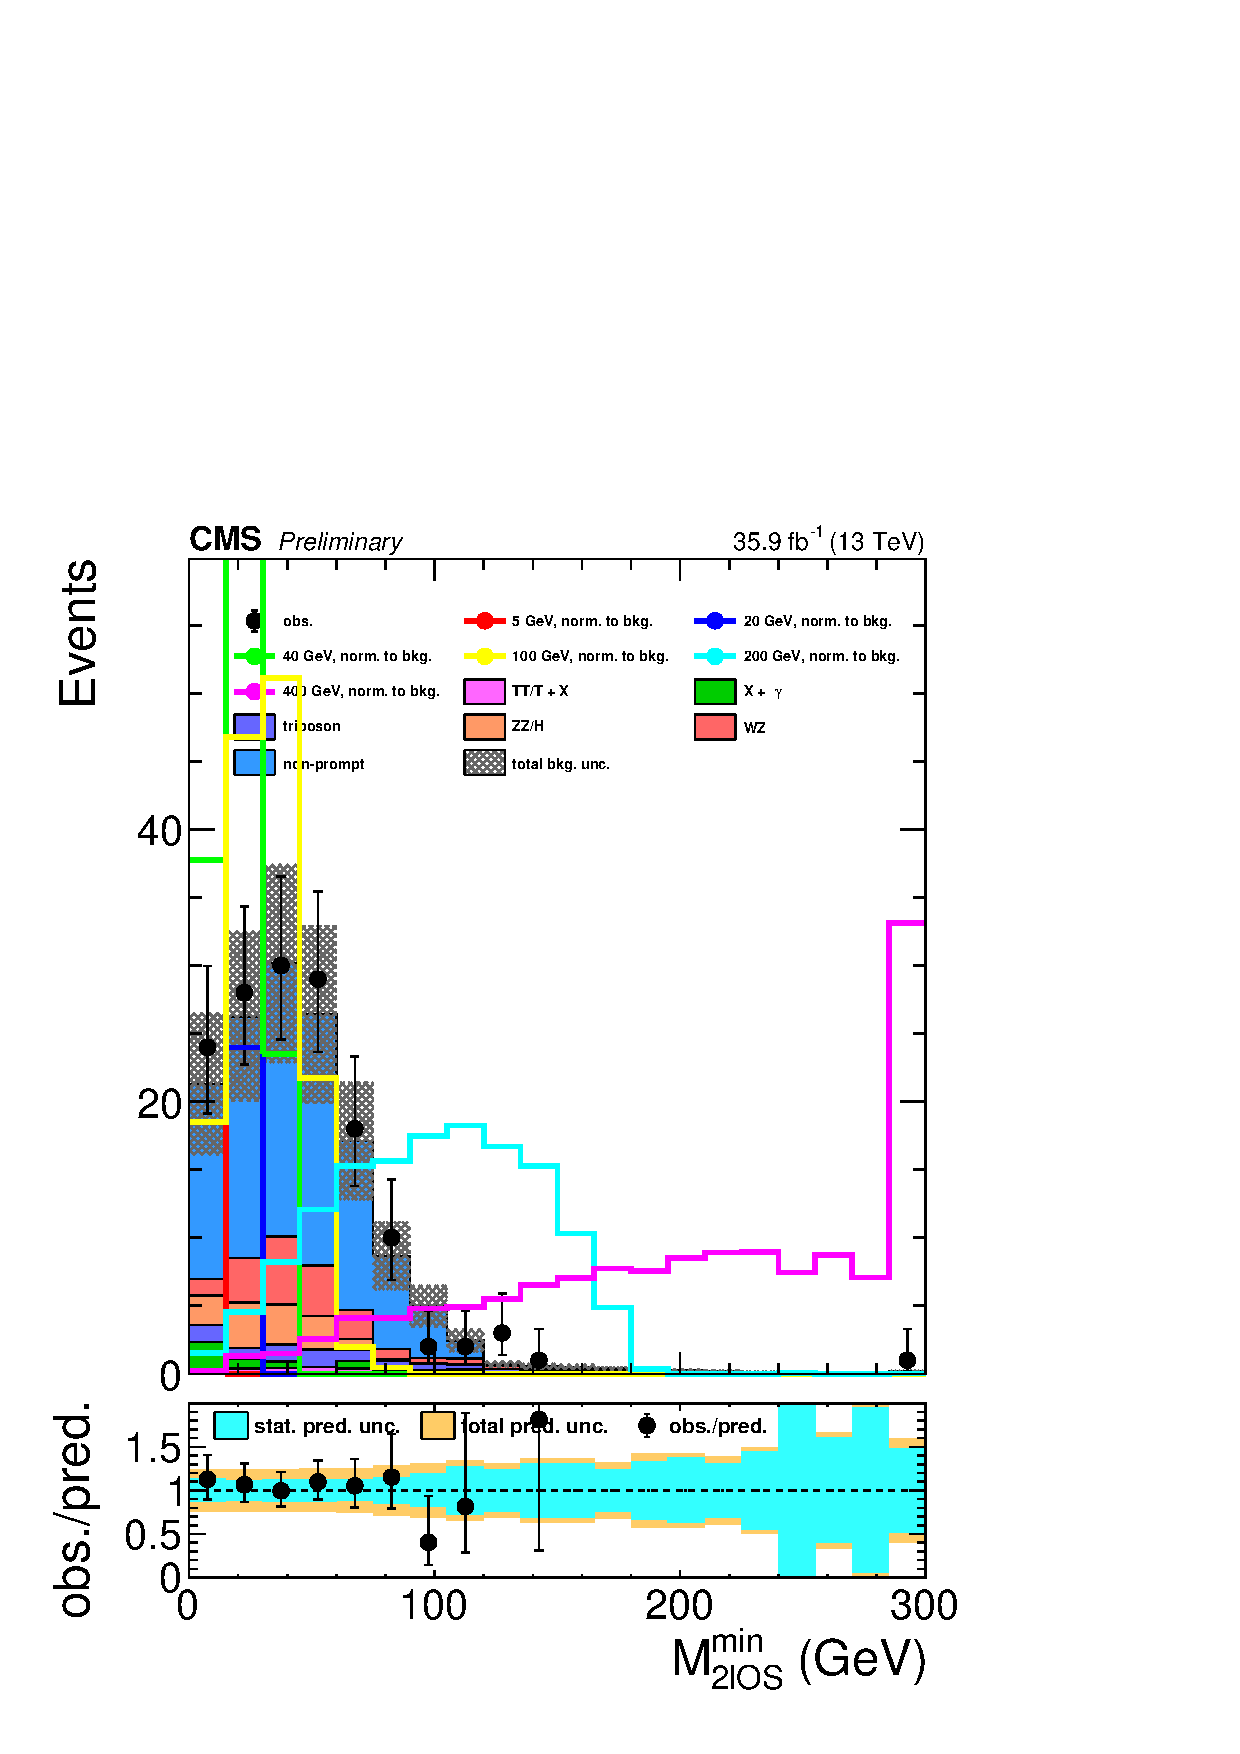
\includegraphics[width=.34\textwidth]{Figures/c5/distribution/minMos_baseline_noOSSF_withSignal.pdf}
  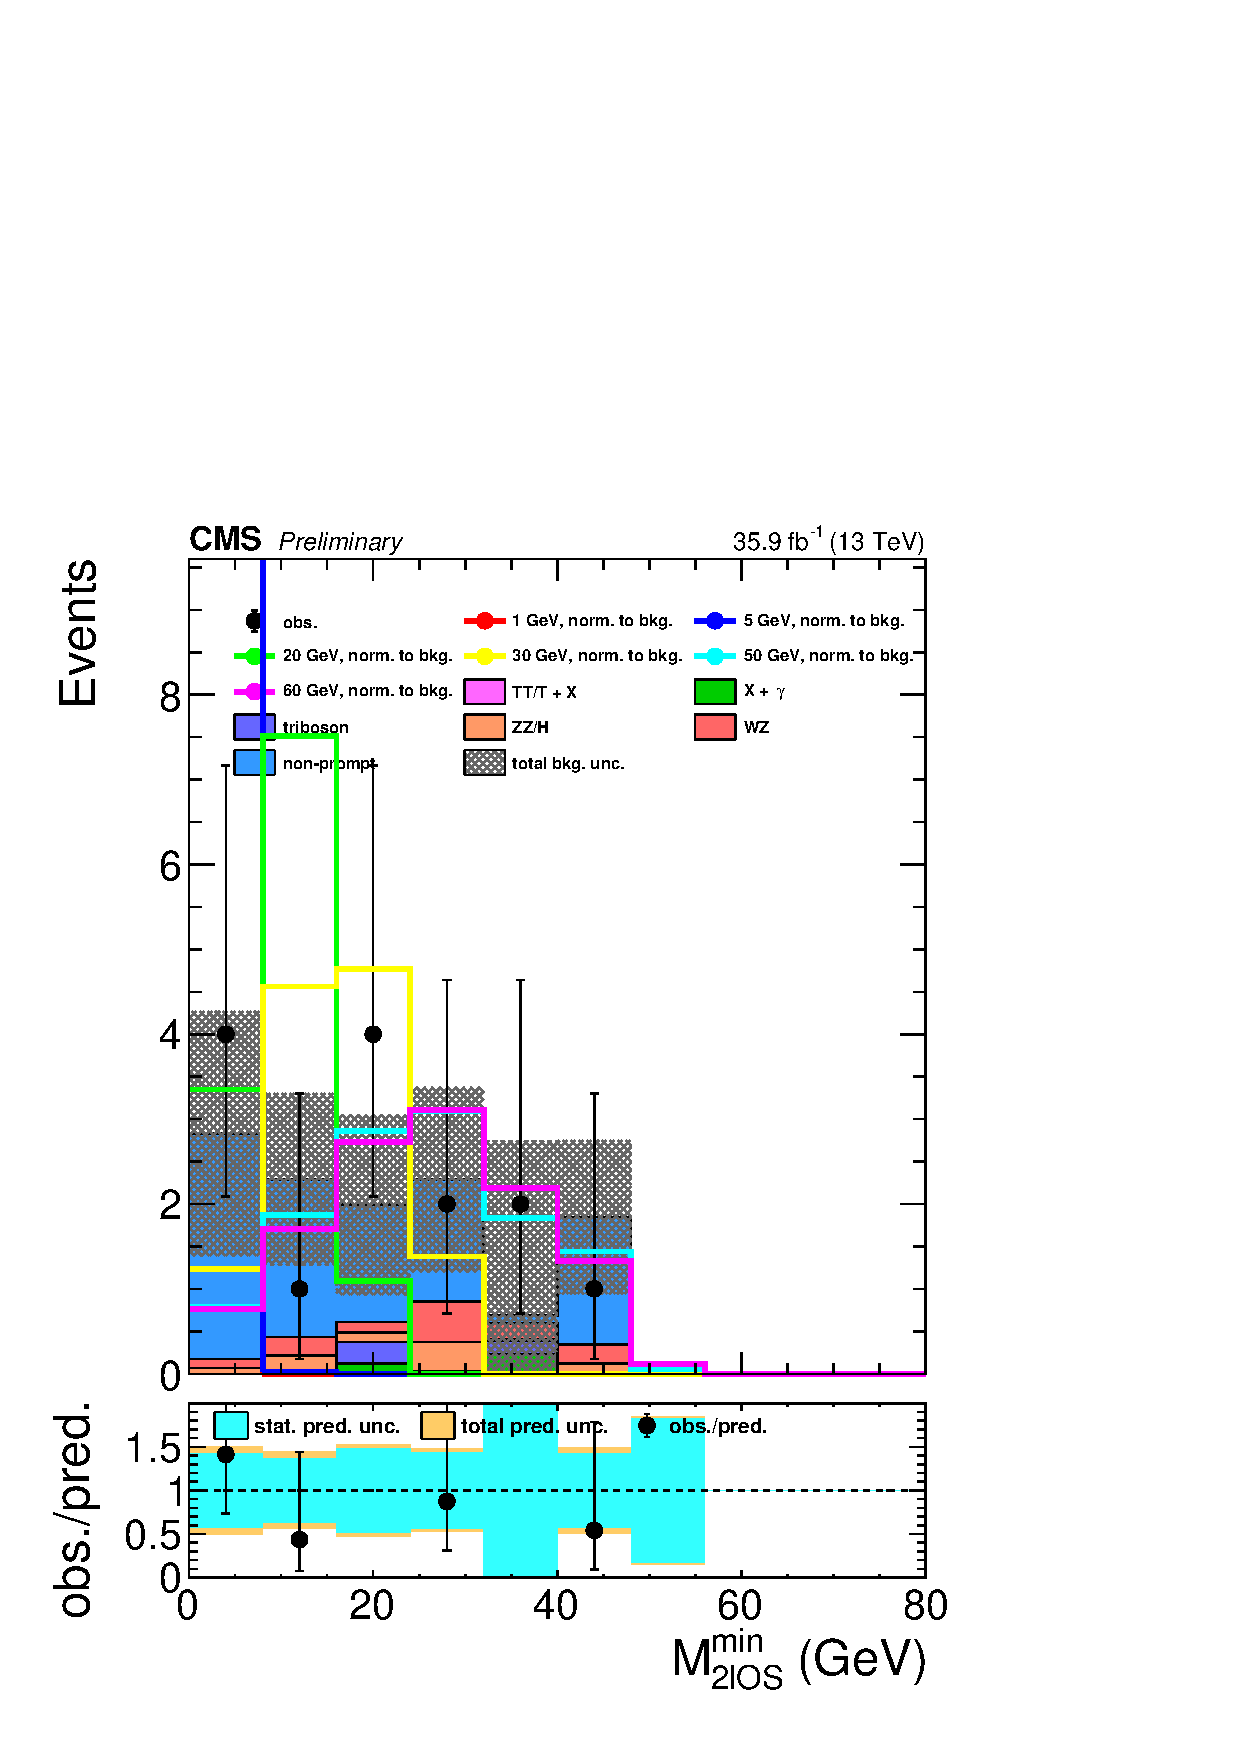
\includegraphics[width=.34\textwidth]{Figures/c5/distribution/minMos_lowM_3lnoOSSF_highPt_withSignal.pdf}
  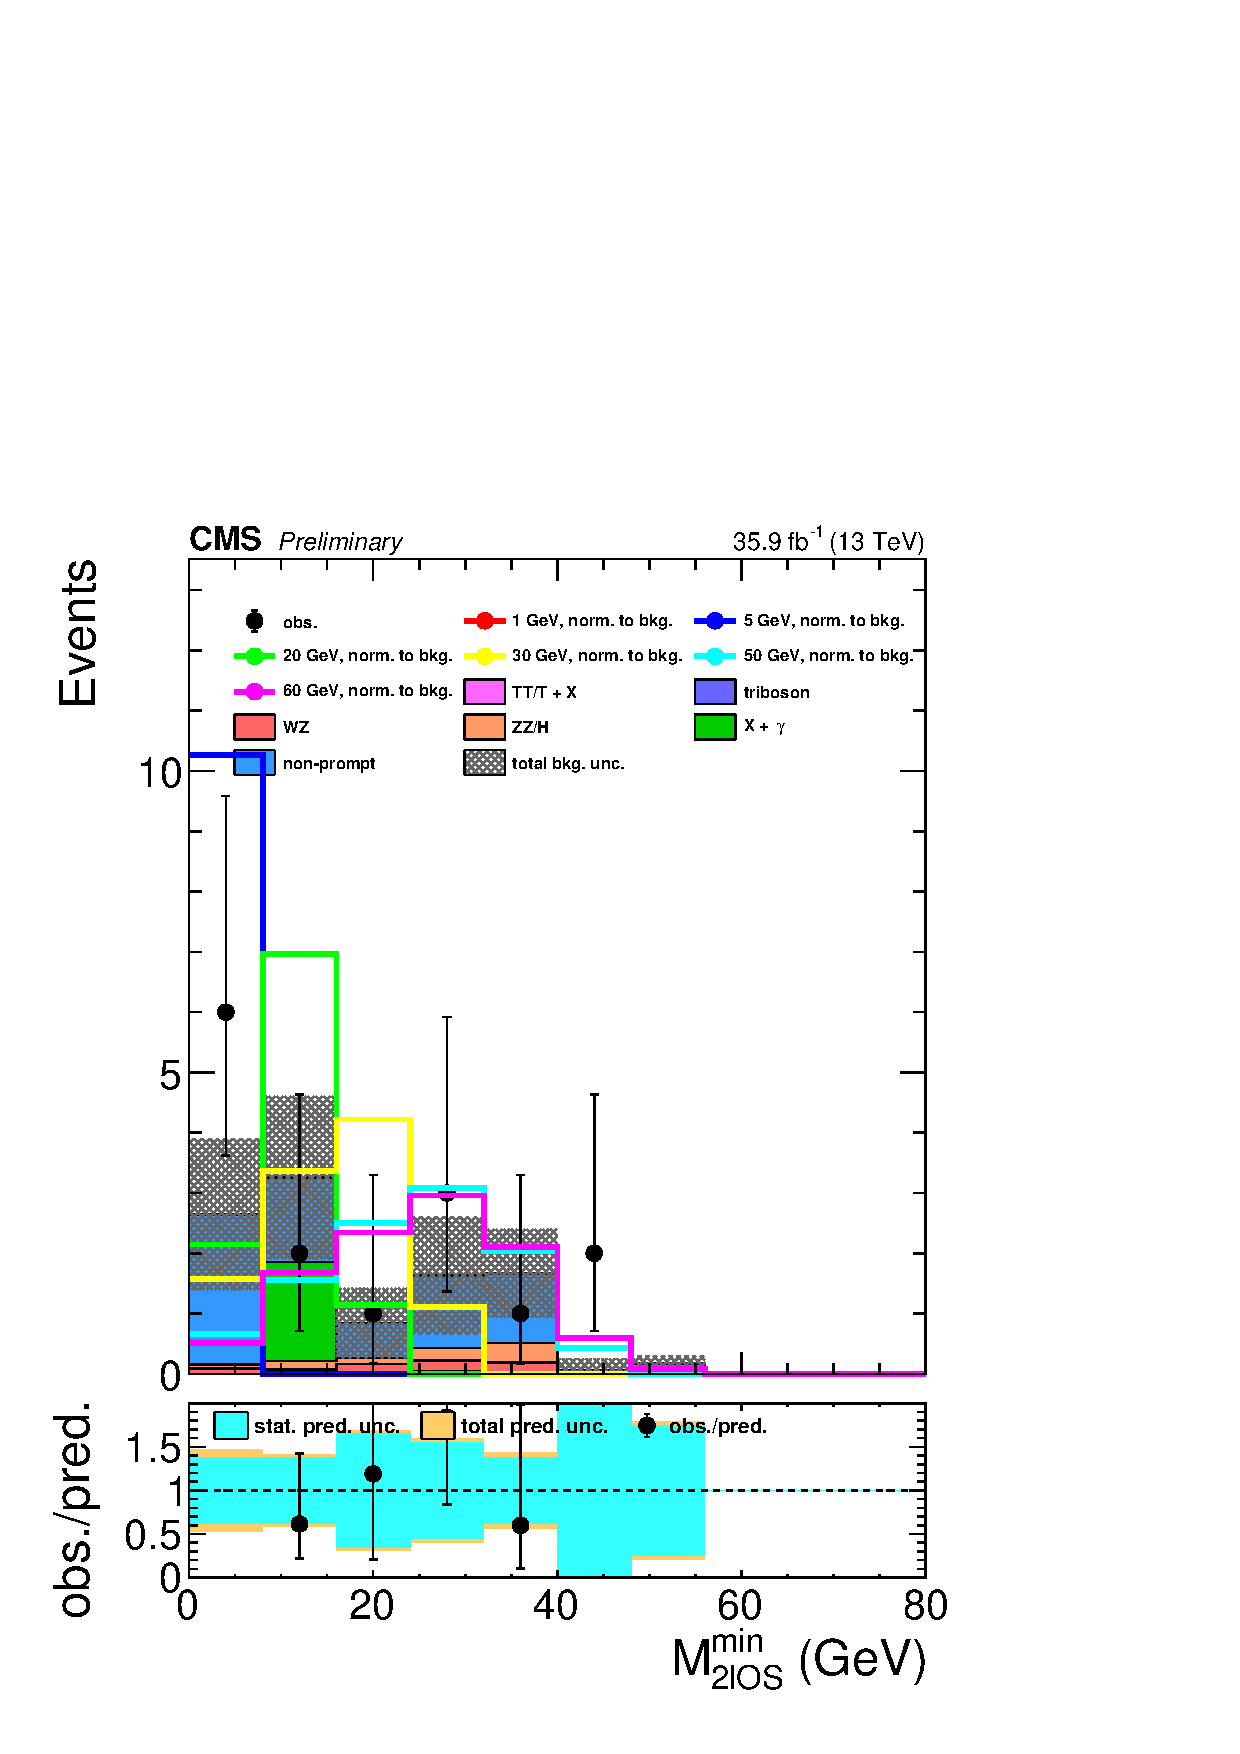
\includegraphics[width=.34\textwidth]{Figures/c5/distribution/minMos_lowM_3lnoOSSF_lowPt_withSignal.pdf}}
  \caption{Expected background yields and signal yields normalized to
  the total background as a function of \mmin for the high leading \pt
  category of the low mass search (middle) and the low leading \pt category
  (right). \willem}
  \label{fig:MminMos}
\end{figure}

The definitions of the low mass
search regions, using this variable, are shown in
Table~\ref{tab:lowMSRdef}. The expected yields in each of these search
regions, compared to the predicted yields of several HNL mass
scenarios, with \mixpar = $10^{-5}$ can be found in Section~\ref{sec:result}.  

\begin{table}[tbh]
\centering
\caption{Search regions in the low mass category.}
\label{tab:lowMSRdef}
\resizebox{0.6\textwidth}{!}{
\begin{tabular}{|c|c|c|c|c|}
\hline
\multirow{2}{*}{$\pt^\text{leading}$ (GeV)}  & \multicolumn{4}{ c| } {\mmin  (GeV)} \\\cline{2-5}
 & $ < 10$ & $10 - 20$ & $20 - 30$ & $> 30$\\
\hline\hline
 $ < 30$ &  SR A1 & SR A2 & SR A3 & SR A4\\ \hline
 $30-55$ &  SR B1 & SR B2 & SR B3 & SR B4\\ \hline
\end{tabular}}
\end{table}



\subsection{High mass search}
To facilitate the simultaneous interpretation of the low- and high mass searches, the selection of events entering each search category should be orthogonal. In the low mass search, the following upper limits are applied to several kinematic quantities: 
\ptmiss < 75\GeV, \pt of leading lepton < 55\GeV and \mlll<
80\GeV. Applying a threshold in \ptmiss to guarantee orthogonality will
cut away a significant portion of the signal, so we opted for using
either the \pt of the leading lepton or \mlll to require
orthogonality. By testing both
orthogonality requirements separately, and computing expected
exclusion limits using the search regions defined further,
 it was established that requiring the \pt of the leading lepton to be
 larger than 55\GeV gave the best performances.
 
In addition to this, the subleading lepton is
 required to pass a \pt threshold of 15\GeV, and the trailing lepton
 is required to be above 10\GeV in \pt .
 This selection requirement somewhat lower the signal acceptance, but drastically
 reduce the background from nonprompt leptons which is especially large for
 very low trailing lepton \pt values. Events in which an OSSF pair is
 present are rejected if \Mll, defined as the OSSF pair mass closest
 to the \PZ mass, falls within a range of 15\GeV around the \PZ boson
 mass, in order to reject the bulk of the $WZ$ background.
 The same off-\PZ requirement is applied to \mlll in order to suppress
 the contribution from the earlier mentioned asymmetric external and
 internal conversions.

The summary of the \emph{high mass} search event selection is listed
in Table~\ref{tab:highMEventSelectio}.

\begin{table}[h]
  \centering
  \caption{\label{tab:highMEventSelectio} Baseline selection requirements
    applied to all data sets for the \emph{high mass} search.}
  \begin{tabular}{l|l}
    \hline
    Variable     & Requirement       \\
    \hline
    \hline
     N. \PQb & = 0              \\
    4th $\ell$ vetoe & \checkmark       \\
    $\pt^{\text{leading}}$ & > 55\GeV\\
    $\pt^{\text{subleading}}$ & > 15\GeV\\
    $\pt^{\text{trailing}}$ & > 10\GeV\\
     $|\mlll - 91|$ & > 15\GeV\\
     $|\Mll - 91|$ & > 15\GeV\\
    \mmin & > 5\GeV\\
    \hline
    \hline
  \end{tabular}

\end{table}


In order to minimize the expected exclusion limits on the HNL mixing
parameter we started by checking a plethora of variables for
discriminating power between the signal and the background. The shapes
of the background and of the signal were compared in all of those
variables, and the most promising variables, giving large and obvious
shape differences were picked out by eye. All the variables displaying
shape differences were then used to design multiple sets of
preliminary search region definitions used for binning the events. The
expected signal exclusion limits were computed for each set of search
regions by performing a simultaneous fit, and compared among the
several preliminary search region definitions. Two variables were found to be more optimal than the others: the earlier mentioned \mmin and the
transverse mass of the lepton not belonging to the pair forming this
minimum mass, referred to as \mtmin. The expected
yields are shown in Figure~\ref{fig:mtminmm3lOSSF} for events
with- and without an OSSF pair, compared to several HNL
mass scenarios with yields normalized to those of the background. 

\begin{figure}[h!]
\centering
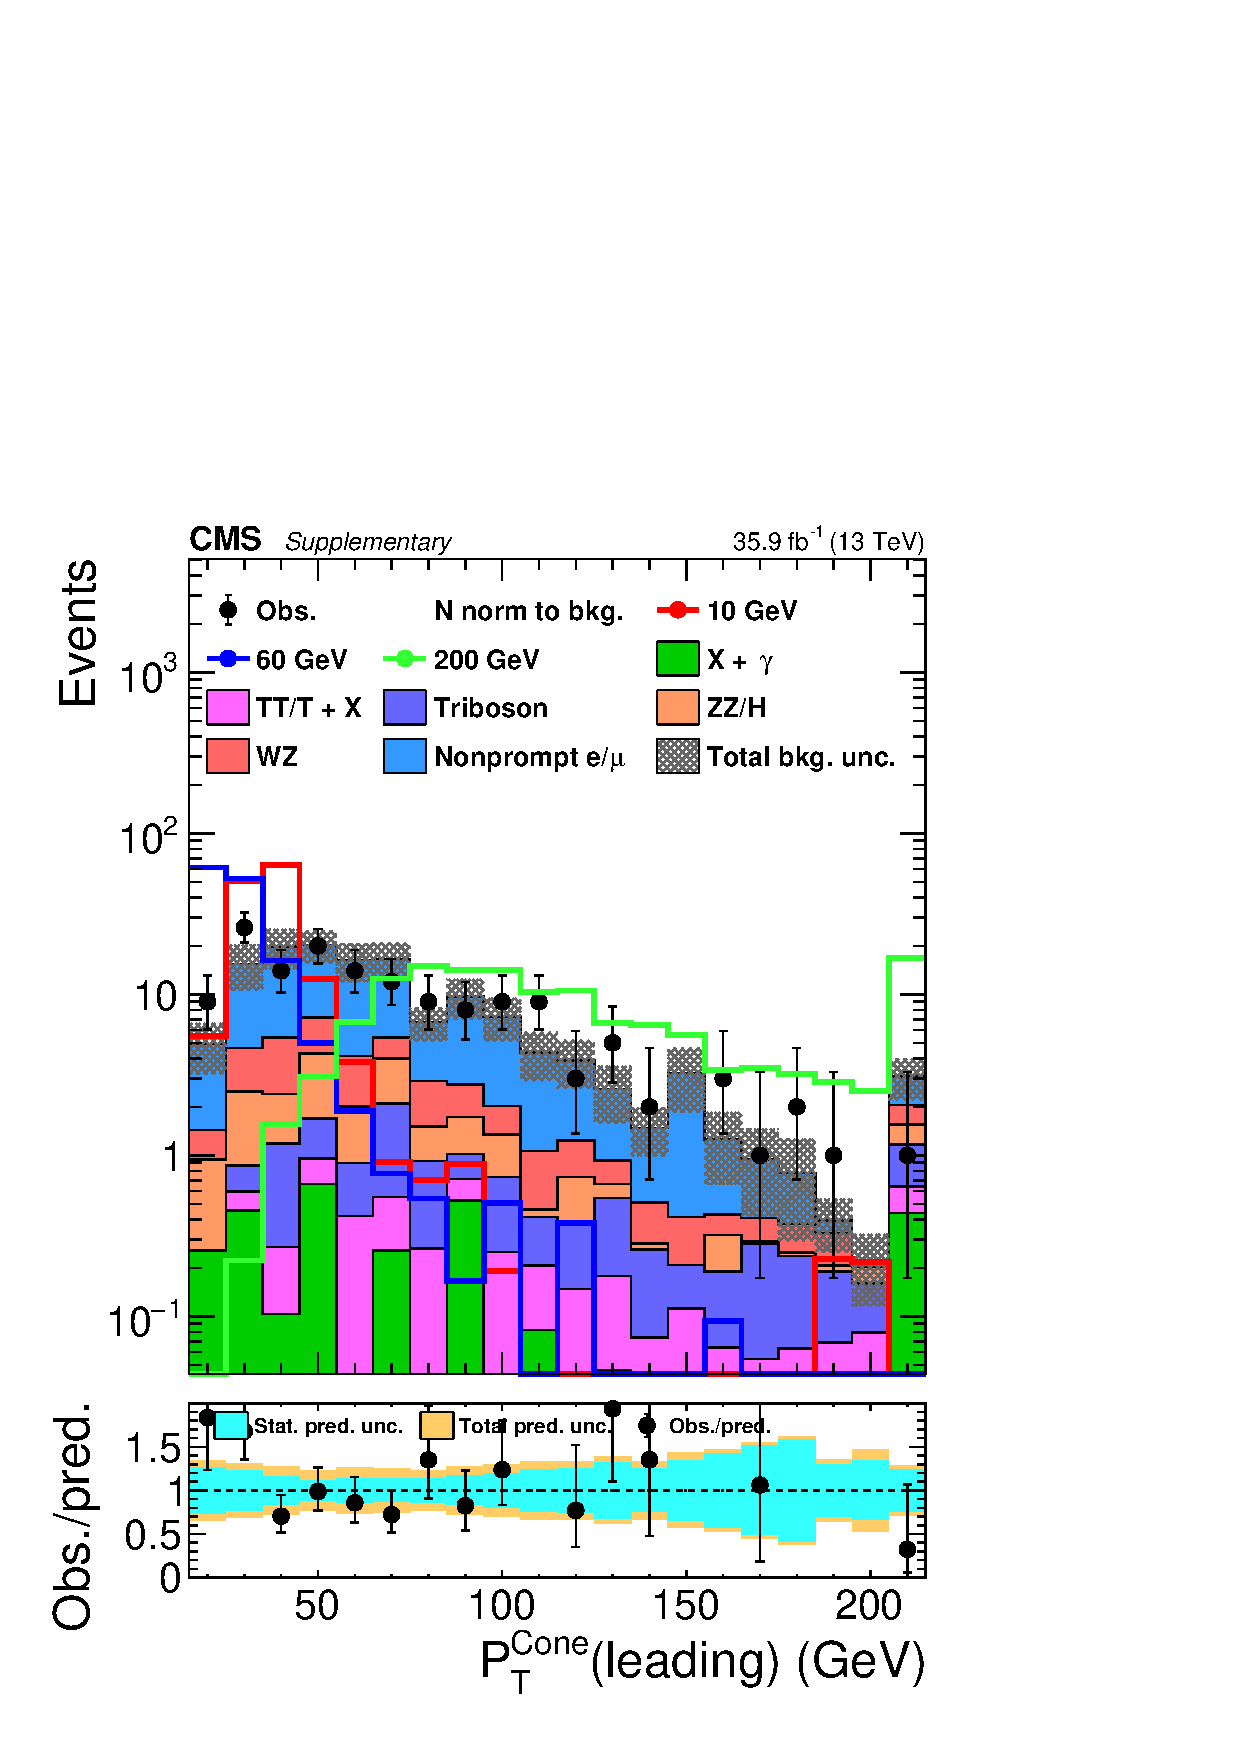
\includegraphics[ width=0.4\textwidth]{Figures/c5/distribution/SR/ConePt_le_baseline_3lnoOSSF_withSignal_sigNormToBkg_log.pdf}
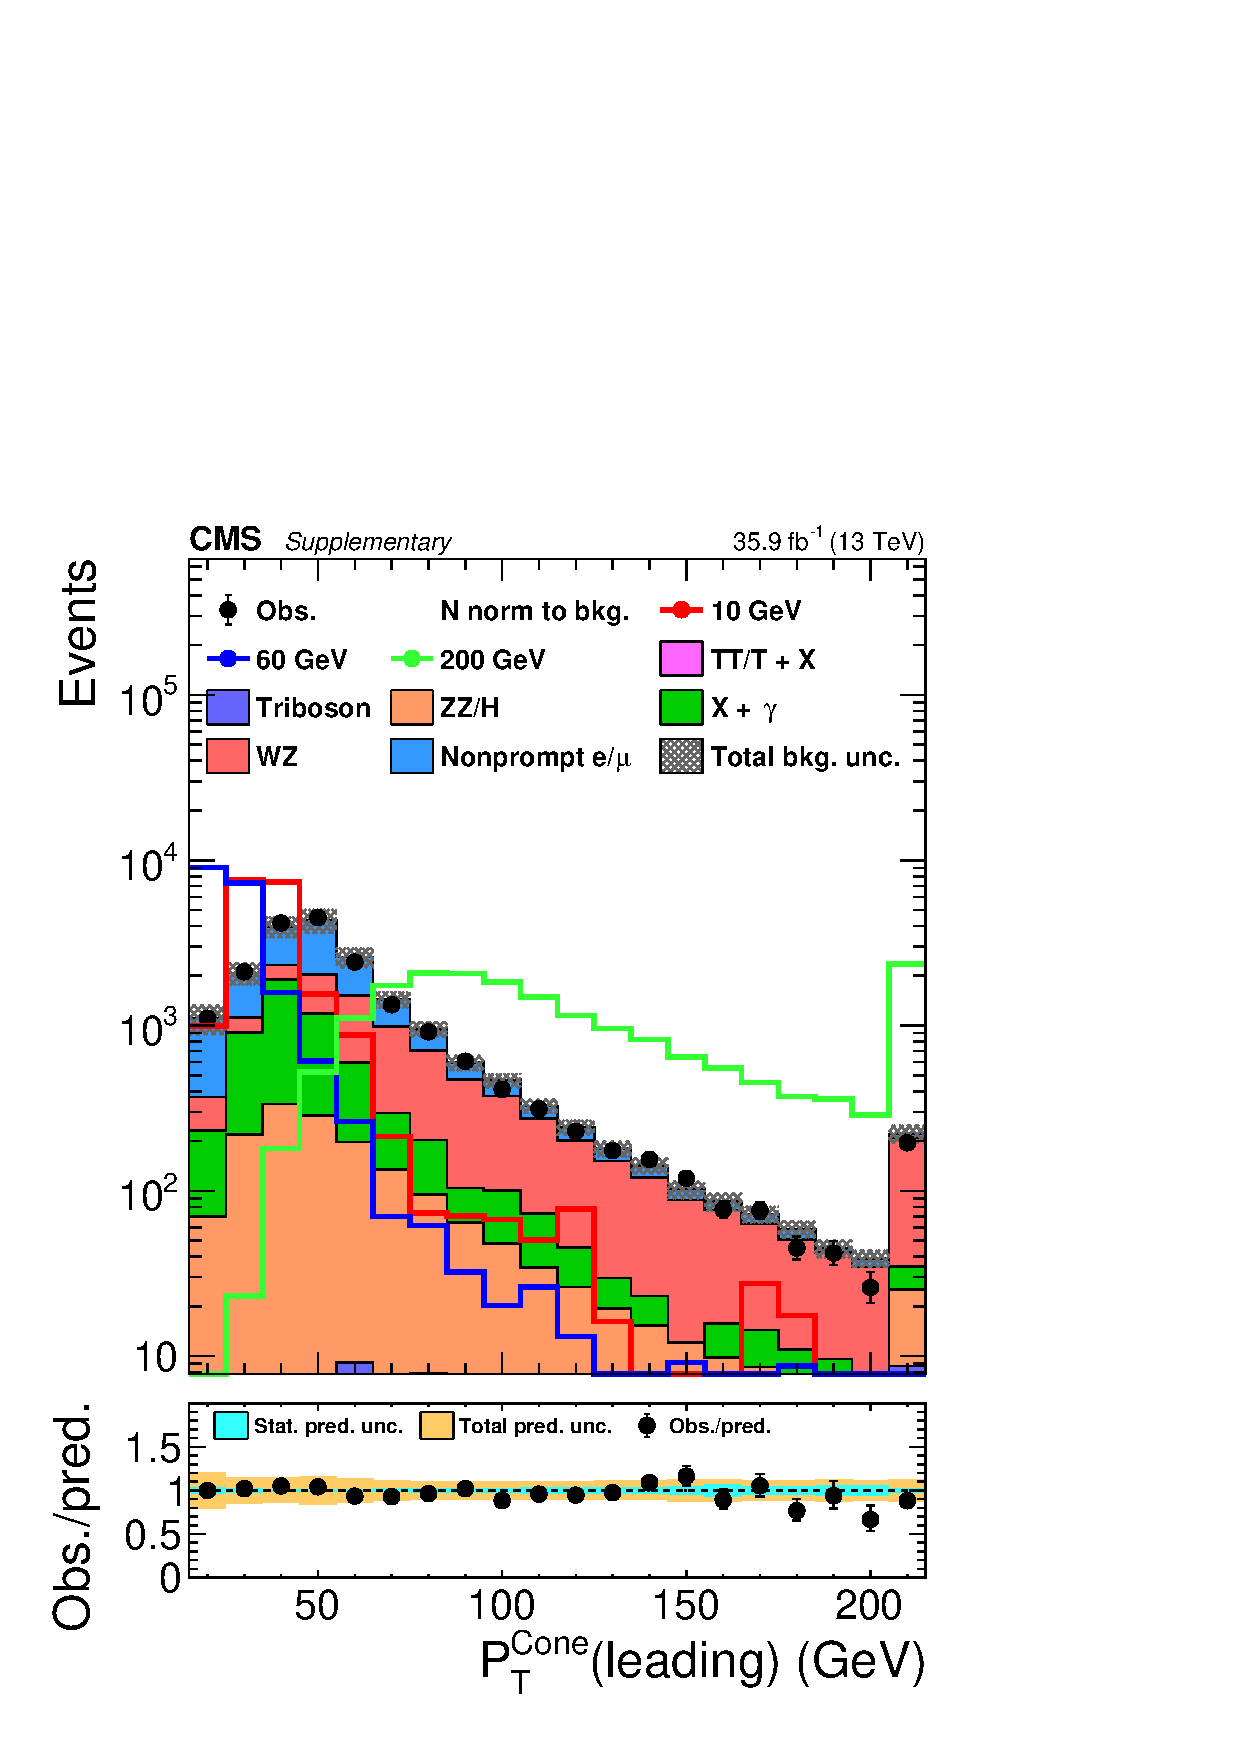
\includegraphics[ width=.4\textwidth]{Figures/c5/distribution/SR/ConePt_le_baseline_3lOSSF_withSignal_sigNormToBkg_log.pdf}\\
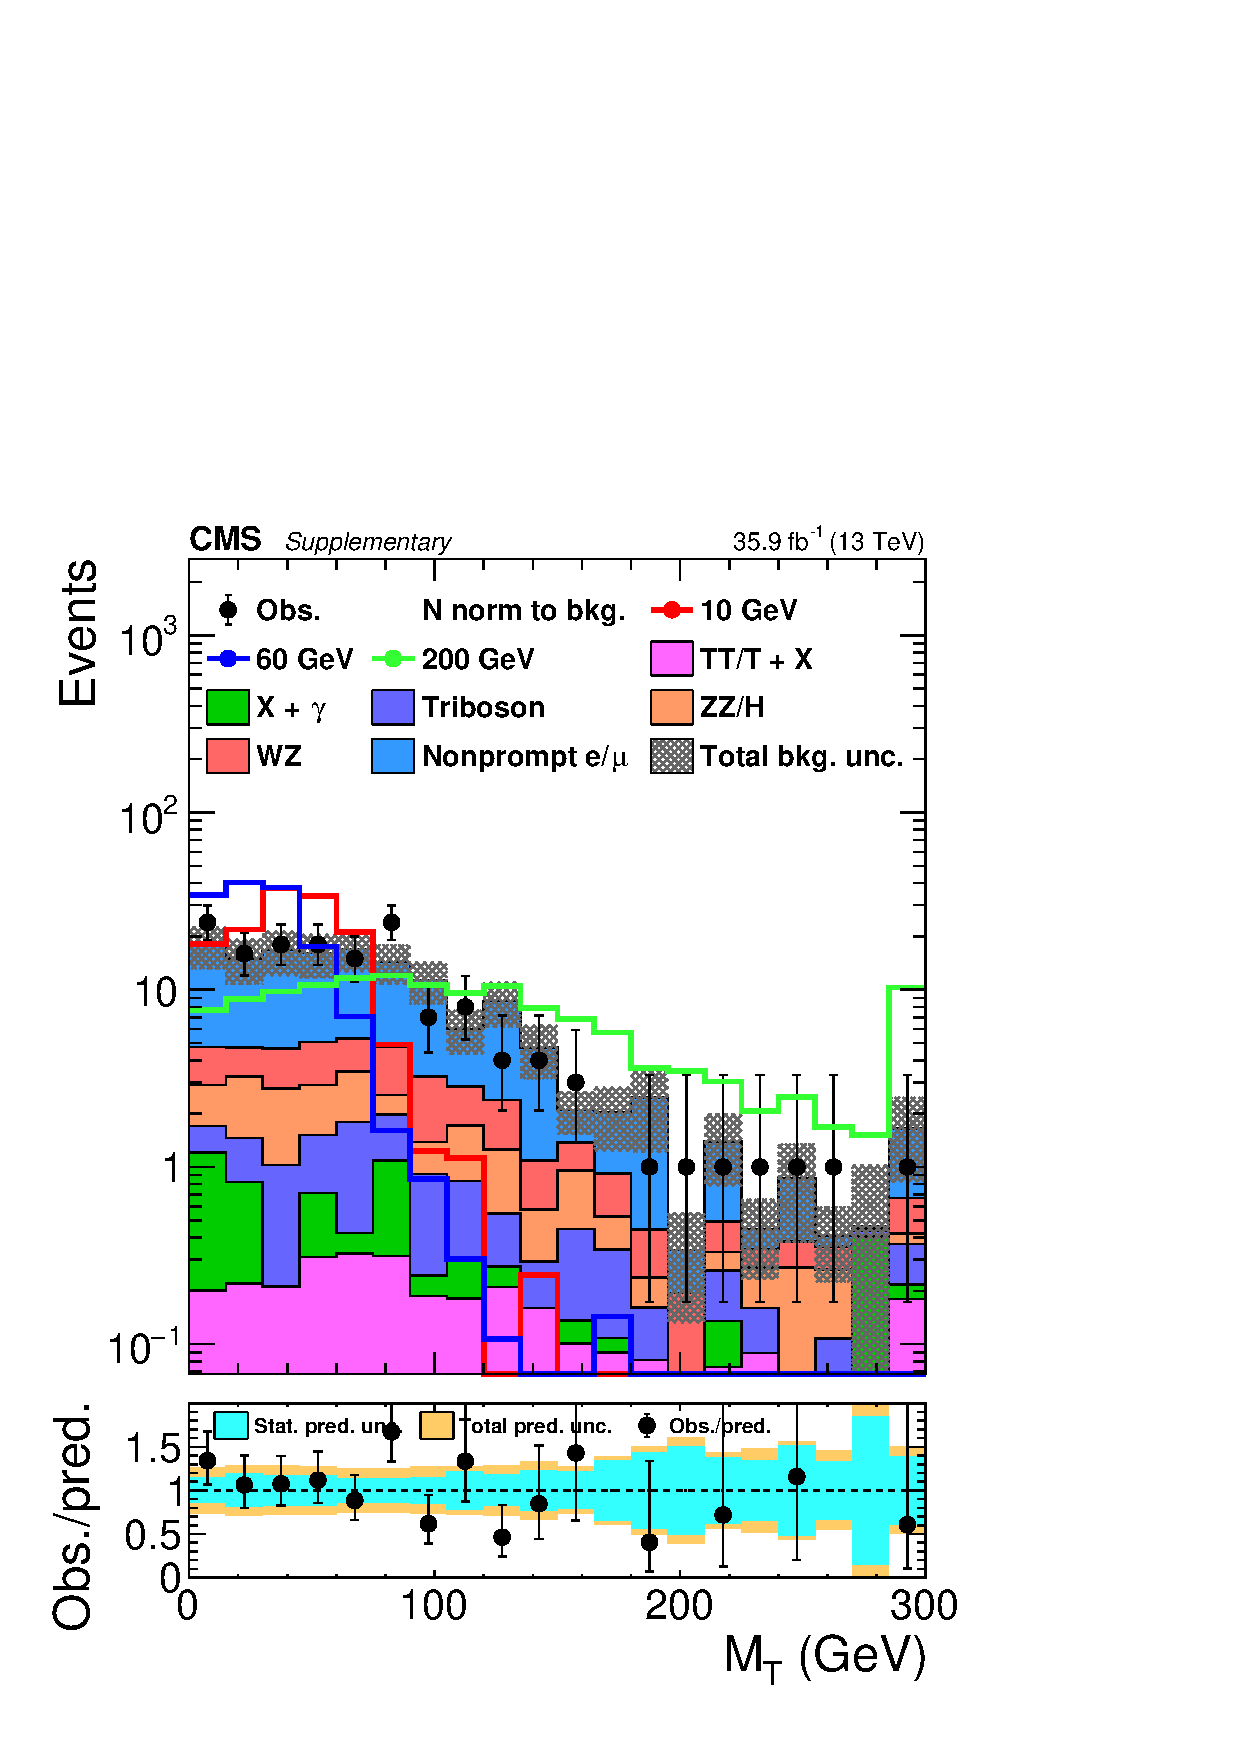
\includegraphics[width=.4\textwidth]{Figures/c5/distribution/SR/mt_minMos_baseline_3lnoOSSF_withSignal_sigNormToBkg_log.pdf}
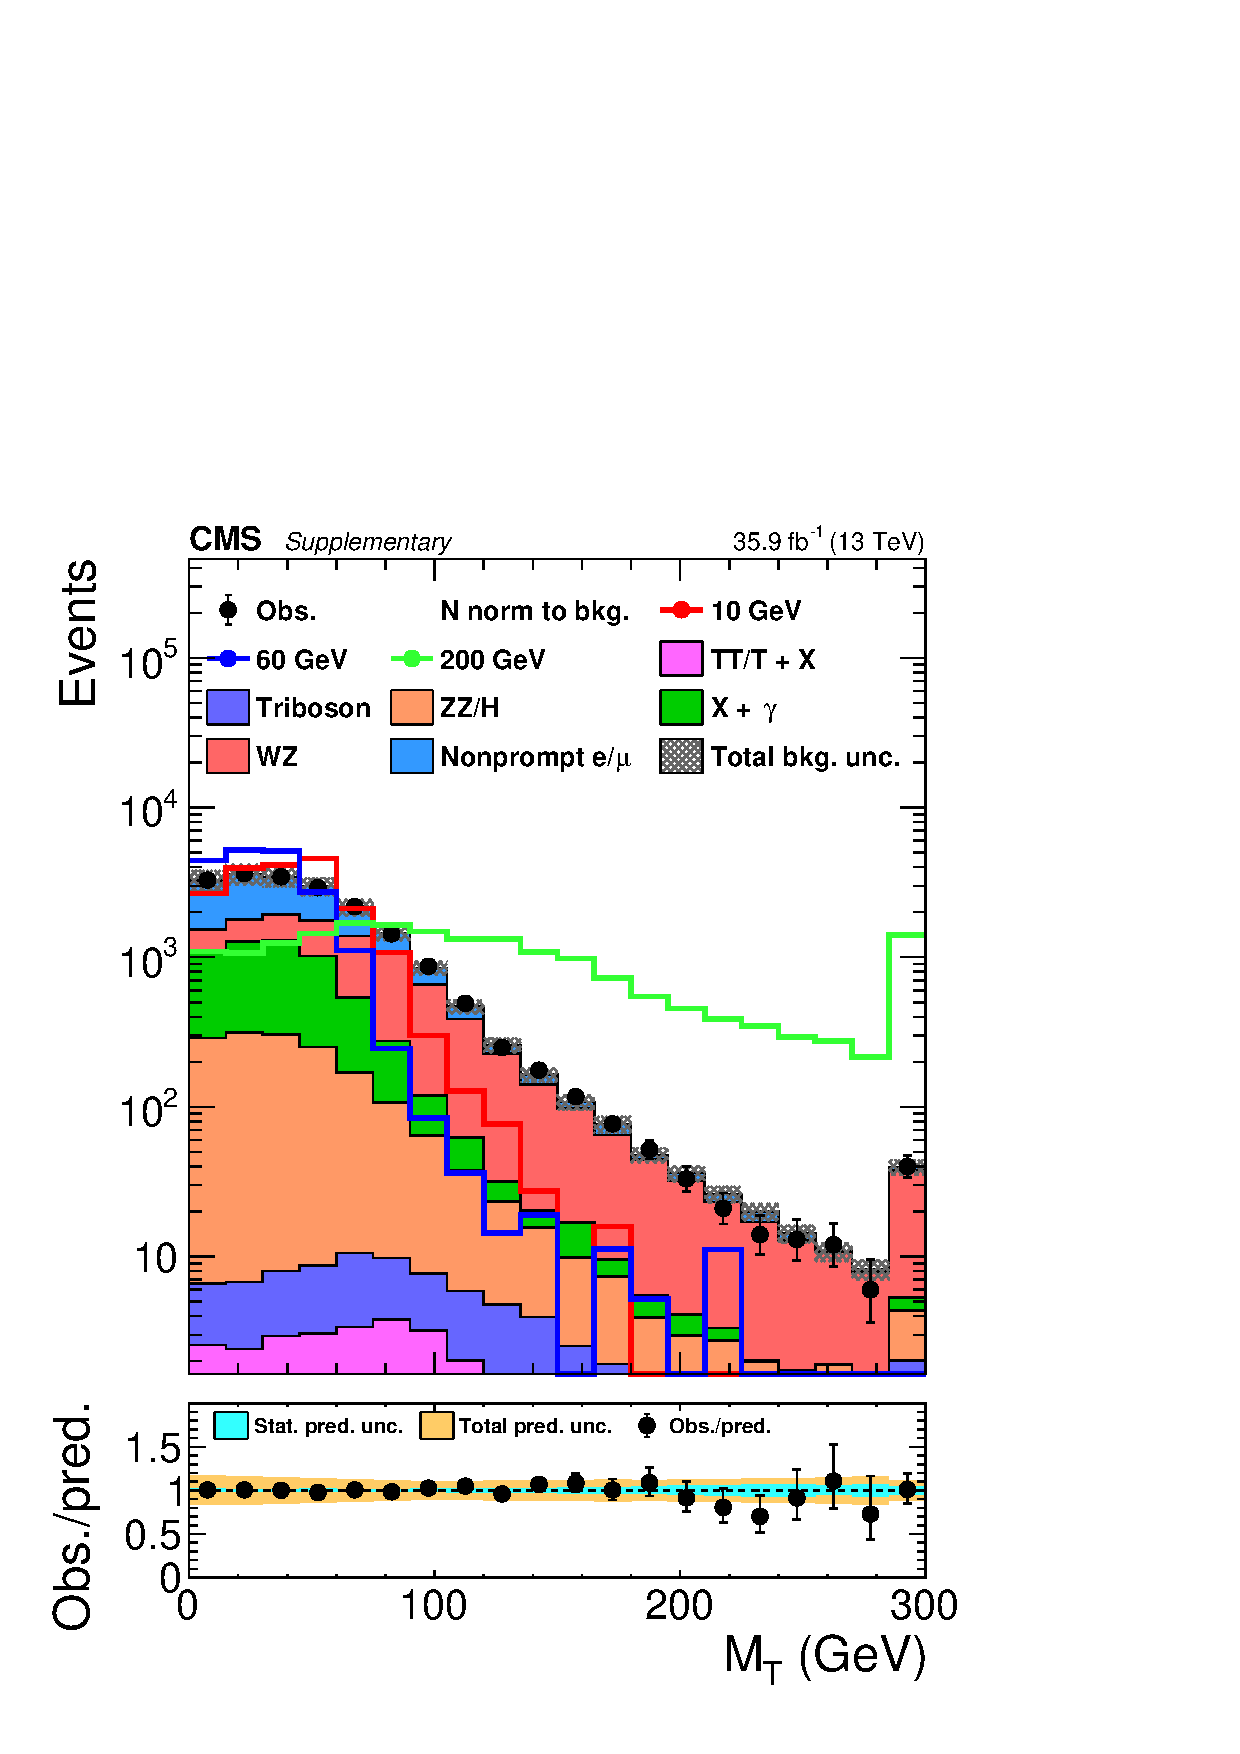
\includegraphics[width=.4\textwidth]{Figures/c5/distribution/SR/mt_minMos_baseline_3lOSSF_withSignal_sigNormToBkg_log.pdf}
\caption{The distributions of \ptcone and \mtmin for
  events without an OSSF pair (left) and with an OSSF pair (right). \willem} 
\label{fig:mtminmm3lOSSF}
\end{figure}

The selection of the search regions was done by defining, in bins of
\mtmin and \mmin, a very large number of search regions which were
iteratively collapsed in order to retain about one background event in
each search region, facilitating correct limit setting and a reliable
background prediction. Events with low
\mlll bin (\mlll < 100\GeV) are expected to significantly contribute to
the sensitivity for HNL masses below the W mass. For events with an
OSSF pair, events with a lepton pair forming a mass below 5
\GeV are vetoed in order to purify the low \mlll bin from a very large
conversion and W$\gamma^{*}$ backgrounds. The search region definitions
are shown in tables ~\ref{tab:SRhighmassOSSF} and
~\ref{tab:SRhighmassnoOSSF}. The expected background yields as a
function of the search region, together with signal yields for several
HNL masses at \mixpar = 10$^{-2}$ can be found in 
Section~\ref{sec:result}.



\begin{table}[h!]
\centering
{\scriptsize
\caption{Search regions for events with an OSSF pair in the high mass category.}
\label{tab:SRhighmassOSSF}
\resizebox{0.6\textwidth}{!}{
\begin{tabular}{|c|c|c|c|c|}
\hline
\multirow{2}{*}{$\mlll$ (GeV)} & \multirow{2}{*}{\mtmin (GeV)} & \multicolumn{3}{ c| } {$\mmin$  (GeV)} \\\cline{3-5}
 & & $ < 100 $ & $100 - 200 $ & $ > 200$\\
\hline\hline
\multirow{3}{*}{$ 0 - 100$}   & $ < 100$ & \multicolumn{3}{c|}{SR C1} \\ \cline{2-5}
	                         & $100-200$ & \multicolumn{3}{c|}{SR C2} \\ \cline{2-5}
                            & $> 200$ & \multicolumn{3}{c|}{SR C3} \\ \hline
\multirow{6}{*}{$> 100$} & $ < 100  $ & SR C4 & SR C9 & SR C13 \\ \cline{2-5}
				                      & $100-200 $ & SR C5 & SR C10 & SR C14 \\ \cline{2-5}
				                     & $200-300 $ & SR C6 & SR C11 & SR C15 \\ \cline{2-5}
				                      & $300-400 $ & SR C7 & \multirow{3}{*}{SR C12} & \multirow{3}{*}{SR C16} \\ \cline{2-3} 									
									 & $>400$ & SR C8 &  & \\ \hline
\end{tabular}}
}
\end{table}

\begin{table}[t!]
\centering
{\scriptsize
\caption{Search regions for events without an OSSF pair in the high mass category.}
\label{tab:SRhighmassnoOSSF}
\resizebox{0.6\textwidth}{!}{
\begin{tabular}{|c|c|c|c|c|}
\hline
\multirow{2}{*}{$\mlll$ (GeV)} & \multirow{2}{*}{$\mtmin$ (GeV)} & \multicolumn{3}{ c| } {$\mmin$  (GeV)} \\\cline{3-5}
 & & $ < 100 $ & $100 - 200 $ & $ > 200$\\
 \hline\hline
\multirow{2}{*}{$ 0 - 100$}  & $ < 100$ & \multicolumn{3}{c|}{SR D1} \\ \cline{2-5}
	                         & $> 100$ & \multicolumn{3}{c|}{SR D2} \\ \hline     
\multirow{4}{*}{$> 100$} & $ < 100  $ & SR D3 & SR D7 & \multirow{4}{*}{SR D9} \\ \cline{2-4}
				                      & $100-150 $ & SR D4 & \multirow{3}{*}{SR D8} &  \\ \cline{2-3}
				                      & $150-250 $ & SR D5 & & \\ \cline{2-3}
				                      & $> 250$ & SR D6  & & \\ \hline								
\end{tabular}}
}
\end{table}
\vspace{5cm}
%%%%%%%%%%%%%%%%%%%%%%%%%%%%%%%%%%%%%%%%%%%%%%%%%%%%%%%%%%%%%%%%%%%%%%%%%%%%%%%%%%%%%%%%%%%%%%%%%%%%%%%
%%%%%%%%%%%%%%%%%%%%%%%%%%%%%%%%%%%%%%%%%%%%%%%%%%%%%%%%%%%%%%%%%%%%%%%%%%%%%%%%%%%%%%%%%%%%%%%%%%%%%%%
%%%%%%%%%%%%%%%%%%%%%%%%%%%%%%%%%%%%%%%%%%%%%%%%%%%%%%%%%%%%%%%%%%%%%%%%%%%%%%%%%%%%%%%%%%%%%%%%%%%%%%%
\section{Background estimation}\label{sec:bgk}
An overview of the principal background contributions is shown in
Figure~\ref{fig:willem3L}.
The main sources of backgrounds (refer to Section~\ref{sec:c4sm} for
an extensive overview) present 
in the final search regions can be divided into the following categories:
\begin{itemize}
\setlength\itemsep{-0.1em}
\item {\bf WZ production:} when both $\PW$ and $\PZ$ bosons decay
  leptonically, these events produce the same signature as the new
  physics scenarios targeted by this analysis: three energetic and
  isolated leptons and a sizable $\ptmiss$ due to a neutrino from the
  $\PW$ boson decay. This is the dominant background by large in the
  searches with three $\Pe$ or $\mu$ forming an OSSF dilepton
  pair. Further details in Section~\ref{sec:promptwz}.

\item {\bf Nonprompt $\Pe$ and $\mu$:} nonprompt leptons are leptons
  from heavy-flavor decays, misidentified hadrons, muons from
  light-mesons that decay in flight, or electrons from unidentified
  conversions of  photons in jets. This background is dominated by the
  \ttbar and Drell-Yan processes. This category provides the largest
  background contribution in the trilepton search regions without an
  OSSF pair. Further details in Section~\ref{sec:tight_loose_method}.

\item {\bf External and internal conversions:} events in which a virtual photon decays (internal conversion) or in which a real photon
converts into leptons by interacting with the detector material
(external conversion). In these cases this photon undergoes an
asymmetric internal or external conversion in which one of the leptons
has very low $\pt$. This soft lepton has a high probability of failing
the selection criteria of the analysis, leading to a reconstructed
two- (in case of a $\PW$ boson) or three-lepton (in case of a $\PZ$
boson) final state. This background mostly contributes to categories
with an OSSF pair. Further details in Section~\ref{sec:conversion}.

\item Rare SM processes with multiple prompt leptons: rare standard
  model processes that yield three or more leptons include multi-boson
  production (\PW, \PZ, $H$), single boson
  production in association with a \ttbar pair, and double-parton
  scattering. Such processes generally have very small production rates
  and in some cases are further suppressed by the b-jet veto. 
\end{itemize}

The background from nonprompt light leptons is estimated by using the \ttol ratio method. 
The probability for a loosely defined light lepton to pass the full
set of
 \begin{wrapfigure}{r}{0.4\textwidth}
\centering
    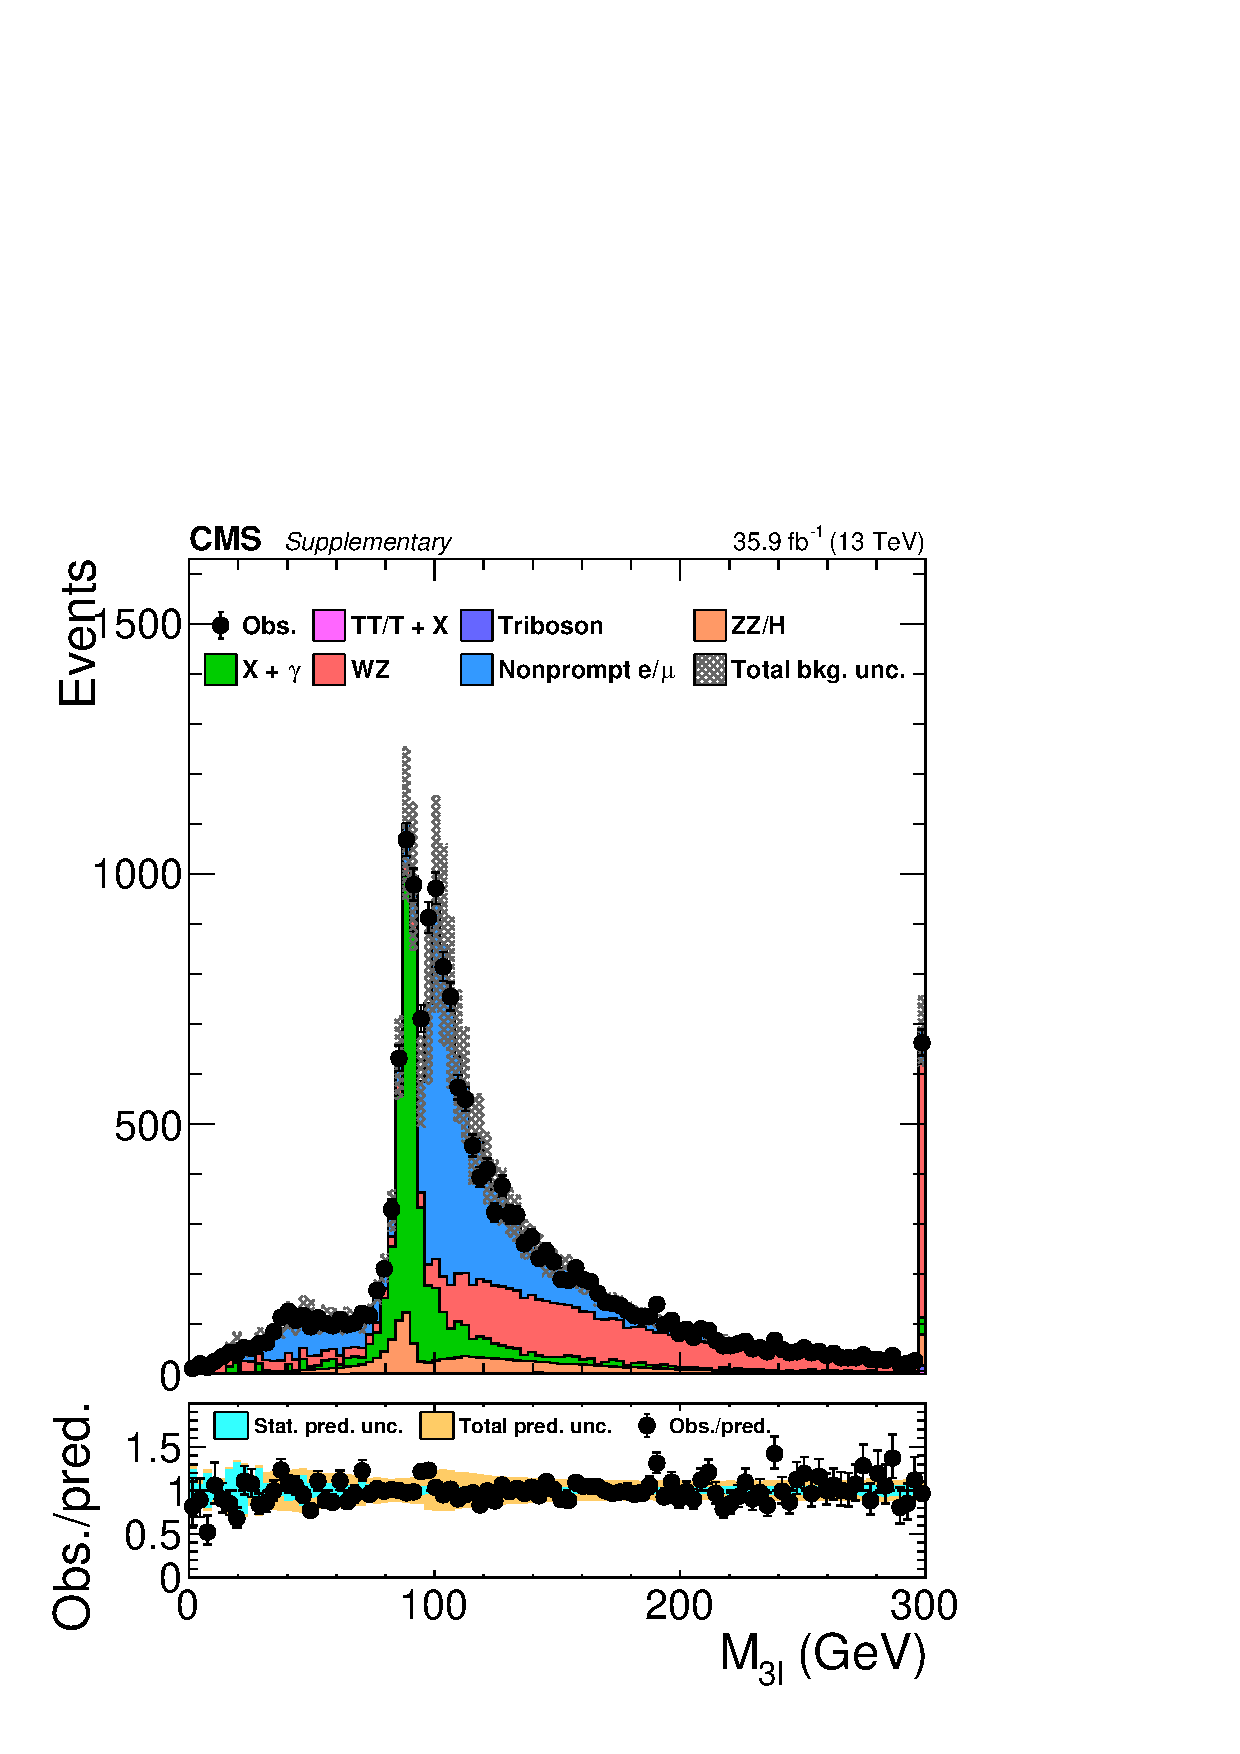
\includegraphics[width=.38\textwidth]{Figures/c5/distribution/SR/M3l_baseline_3lOSSF_noSignal_lin.pdf}
\caption{Observed and expected yields as a function of $\mlll$
for events with an OSSF lepton pair. \willem}
\label{fig:willem3L}
\end{wrapfigure}
 selection criteria is measured in a multi-jet sample in data enriched
 in nonprompt leptons, called the measurement region, refer to
 Section~\ref{sec:tight_loose_method} for details.
Once measured, this probability is applied in a sample of events which
pass the full kinematic selection, but where at least one of the
leptons fails the nominal selection but passes the \fo requirements
(refer to Tables~\ref{tab:muonIDs}-~\ref{tab:eleIDs}), 
in order to predict the number of events from nonprompt leptons entering each search region. 
The residual contribution from prompt leptons in the measurement and application regions is subtracted using MC simulation. 
It is verified in both MC simulation and $\ttbar$- or DY-enriched data control regions that this method describes the background from the nonprompt leptons entering the different search regions within 
a systematic uncertainty of 30\%. 
 
The modeling of the conversion background is verified in a data control region enriched in both external and internal conversions. 
The rate of $\PZ \to 3\ell$ events where one lepton from $\gamma^{(*)}\to\ell\ell$ is out of acceptance is compared with 
the full prediction derived from the MC simulation and the nonprompt leptons estimation method, in an off-Z control region 
defined by |\Mll $- \:M_\PZ$| < 15\GeV, |\mlll $- \:M_\PZ$| < 15\GeV,
and \ptmiss < 50\GeV. 

The \WZ background is normalized to data in a control region obtained 
requiring an on-Z OSSF pair to be present. An additional requirement applied 
for events to enter the control region is \ptmiss > 50\GeV.

The predicted background yields are found to agree with the simulation
within the statistical uncertainties. 

Figure~\ref{fig:willem3L} shows the background composition at the
first stage of the analysis selection.


\subsection{Background from nonprompt and fake leptons}\label{sec:tight_loose_method}

The contribution from nonprompt leptons is derived with the \ttol method
by using event yields with three leptons where at least one lepton fails to satisfy \ti 
selection criteria (refer to
Tables~\ref{tab:muonIDs}-~\ref{tab:eleIDs}) but passes
\fo~\footnote{We all agree that \ttol naming is not optimal when the
  ratio happens between \ti and \fo leptons. For ``historical'' and ``traditional''
  reasons we use \ttol name keeping in mind that the selection in the
  denominator is the \fo one.}
ones (\emph{application region}), 
and by applying to them a \ttol ratio or a \fr (FR
or $f$) which is the probability for 
a nonprompt lepton to pass the \ti and isolation selection.\\
This ratio is constructed in such a way that eliminates the mother parton \pt and flavor dependence.
Hence, while measured in the dijet events, it allows to reliably estimate nonprompt lepton background
arising both from $\ttbar$ and DY+jets processes. \\
To mitigate \fr dependence on the mother parton \pt, the \fr is defined as a function
of a quantity which serves as a proxy for mother parton \pt for non-isolated leptons, and which
is equal to a lepton \pt for isolated leptons. This quantity is
constructed as lepton \pt plus 
the activity in the isolation cone around the lepton, and is thus referred to as \ptcone:

\begin{equation}
\ptcone = \pt^\ell\times\Bigl(1+ \min\bigl(0., \Irel - \Irel^\text{tight}\bigr) \Bigr)
\end{equation}

\noindent where the $\Irel$ is the relative isolation of the lepton
calculated in cone with size $\Delta R=0.3$, while the
$\Irel^\text{tight}$ is the \ti  working point defined in tables~\ref{tab:muonIDs} and \ref{tab:eleIDs}.
In the application region, \ptcone is used to compute all lepton-related kinematic variables
such as $\Mll$, $\MT$ etc., as well as is used instead of the lepton \pt when applying 
search regions \pt thresholds.

Flavor dependence of the \fr is important in the estimation of
nonprompt electrons. While the nonprompt muons are mainly real muons
coming from semileptonic b-decays, the nonprompt electrons are often
misidentified light-flavor jets. The contribution of this source of misidentified light-flavor jets varies significantly between 
the FR measurement multijet region and between the various signal
regions used in this analysis. Minimize the
dependency of the results of the method to the composition of
nonprompt electrons is then necessary; hence the definition
of \fo electron is tuned in such a way that FR for real electrons from semileptonic b-decays
is close to the FR for misidentified jets in the kinematic region of interest to the analysis. 
This tuning is performed by using $\ttbar$ and QCD MC samples, and is
done by finding a working point of 
electron MVA classifier which leads to the desired effect. 

\subsubsection{\fr measurement} \label{sec:singleFR}
We measure the \fr maps in data.\\
The control region we use to measure is enriched in QCD jet events and
it is defined:
\begin{itemize}
\setlength\itemsep{-0.2em}
  {\footnotesize
	\item one \fo (defined in Tables~\ref{tab:muonIDs} and \ref{tab:eleIDs});
	\item at least one jet with $\Delta R$ (jet,FO) $>1$;
	\item $\ptmiss < \ 20$ GeV and $\MT < \ 20 $ GeV;
	\item pass a specific single leptons trigger with \pt thresholds:
          3,8,17\GeV for $\mu$ and 8,12\GeV for electrons.}
\end{itemize}
While measuring the \fr in data in lepton+jet events we should take into account the contamination from prompt leptons, mostly from $\PW$ and $\PZ$ production in association with jets.
 To discriminate between QCD events and $\PW$/$\PZ$ events we can use the transverse mass of the lepton and the missing transverse energy; requiring $\ptmiss$ and $\MT$ upper limits we strongly reduce
  the contribution from prompt leptons in the measurement region. \\
The residual contamination is subtracted both from the numerator and from the denominator transverse momentum bins using the simulated $\PW + \ jets$, DY and $\ttbar$ events from MC samples. The simulation is normalized in the control region dominated by $\PW + \ jets$, DY processes, with $\ptmiss > \ 20$ GeV and $70 \ < \MT < \ 120 $ GeV.
Due to different trigger pre-scales of the single lepton triggers, the
MC normalization and the prompt leptons contribution subtraction are
performed separately for all triggers in the corresponding lepton \pt ranges.


\comm{
\begin{figure}[h!]
\centering
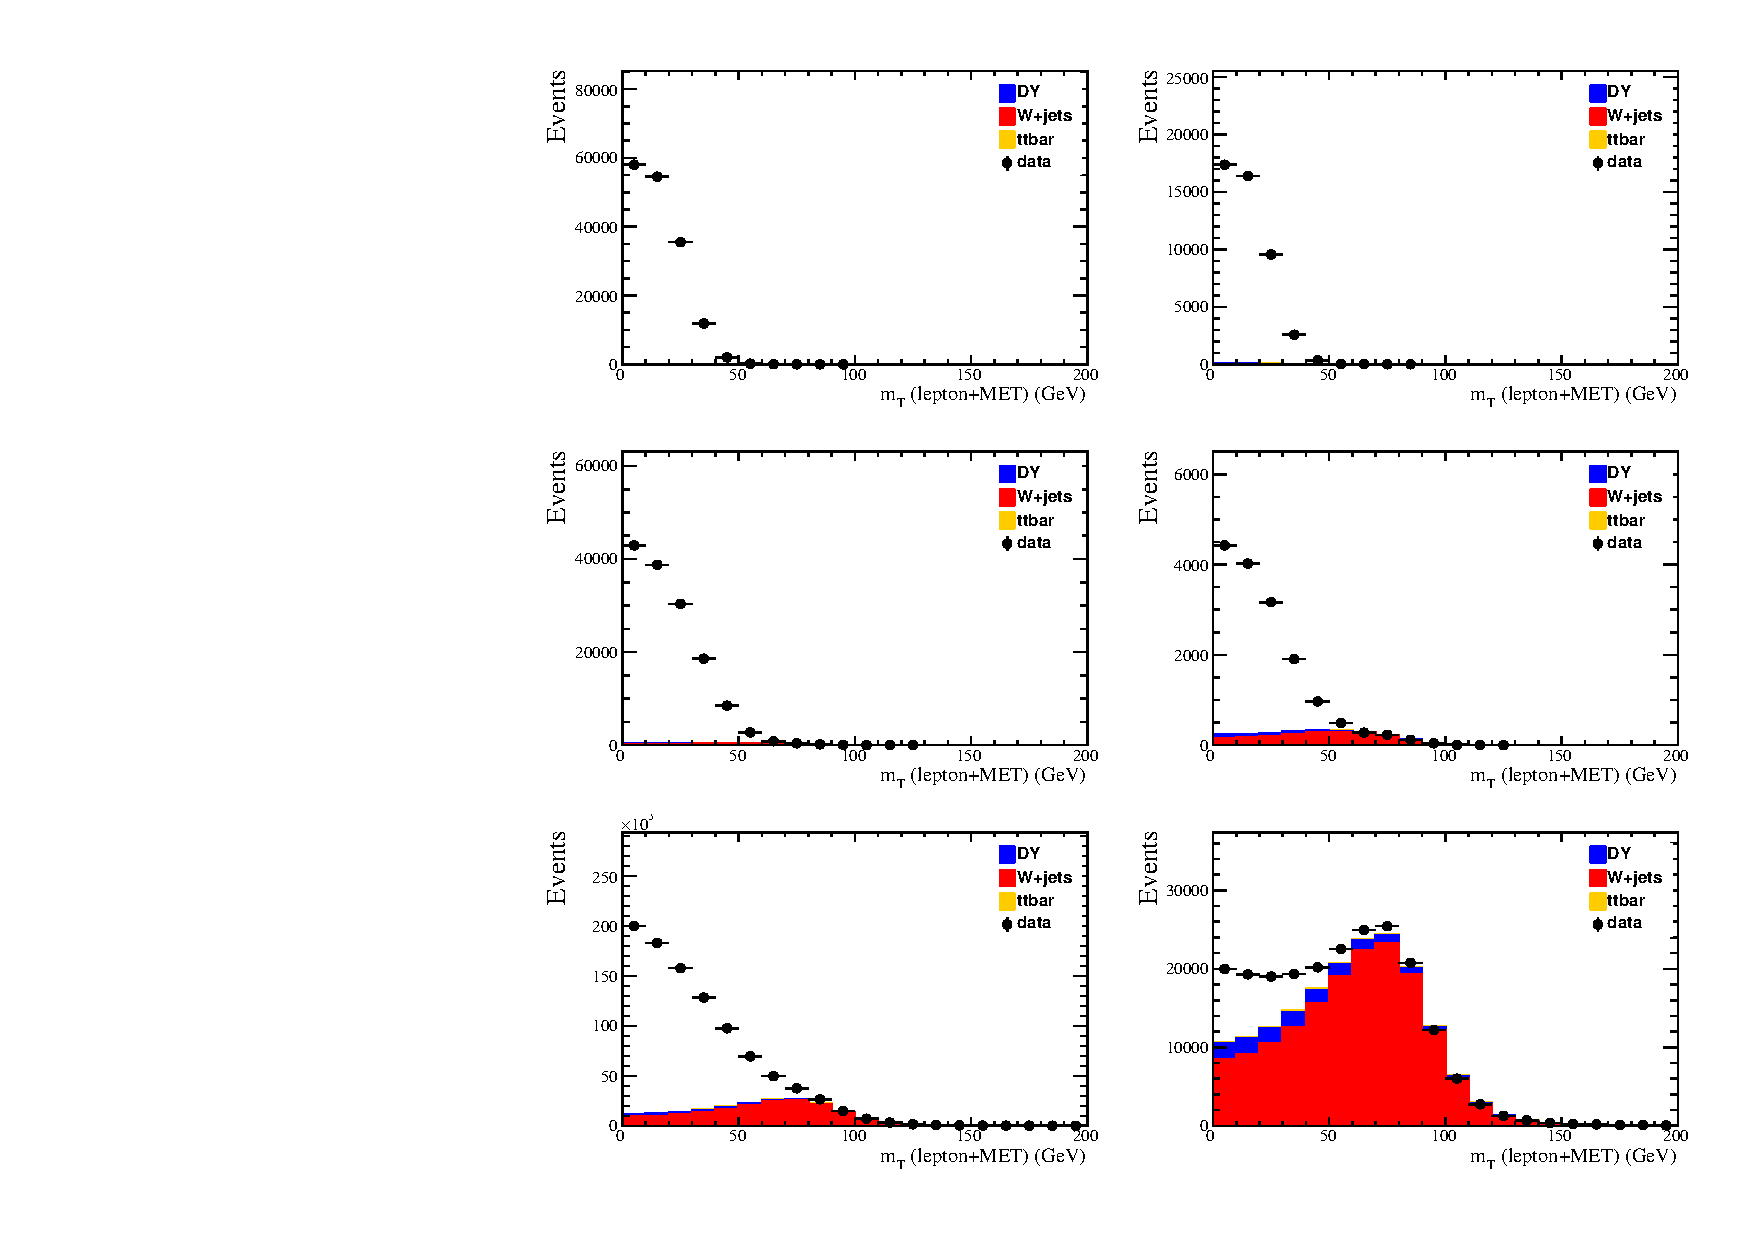
\includegraphics[width=.5\textwidth]{Figures/c5/FAKE/muon_mt.pdf}
\caption{$\MT$ distributions for muons. In the left column there are
  transverse mass distributions for \fo (denominator) while in the
  right one for \ti  leptons (numerator). Three rows for the three muon triggers: Mu3, $\ptcone  \in 
  [5,12]$\GeV, Mu8 $\ptcone  \in 
  [12,25.5]$\GeV and Mu17 $\ptcone  > 25.5$\GeV.}
\label{fig:mt_fake_muon}
\end{figure}

\begin{figure}[h!]
\centering
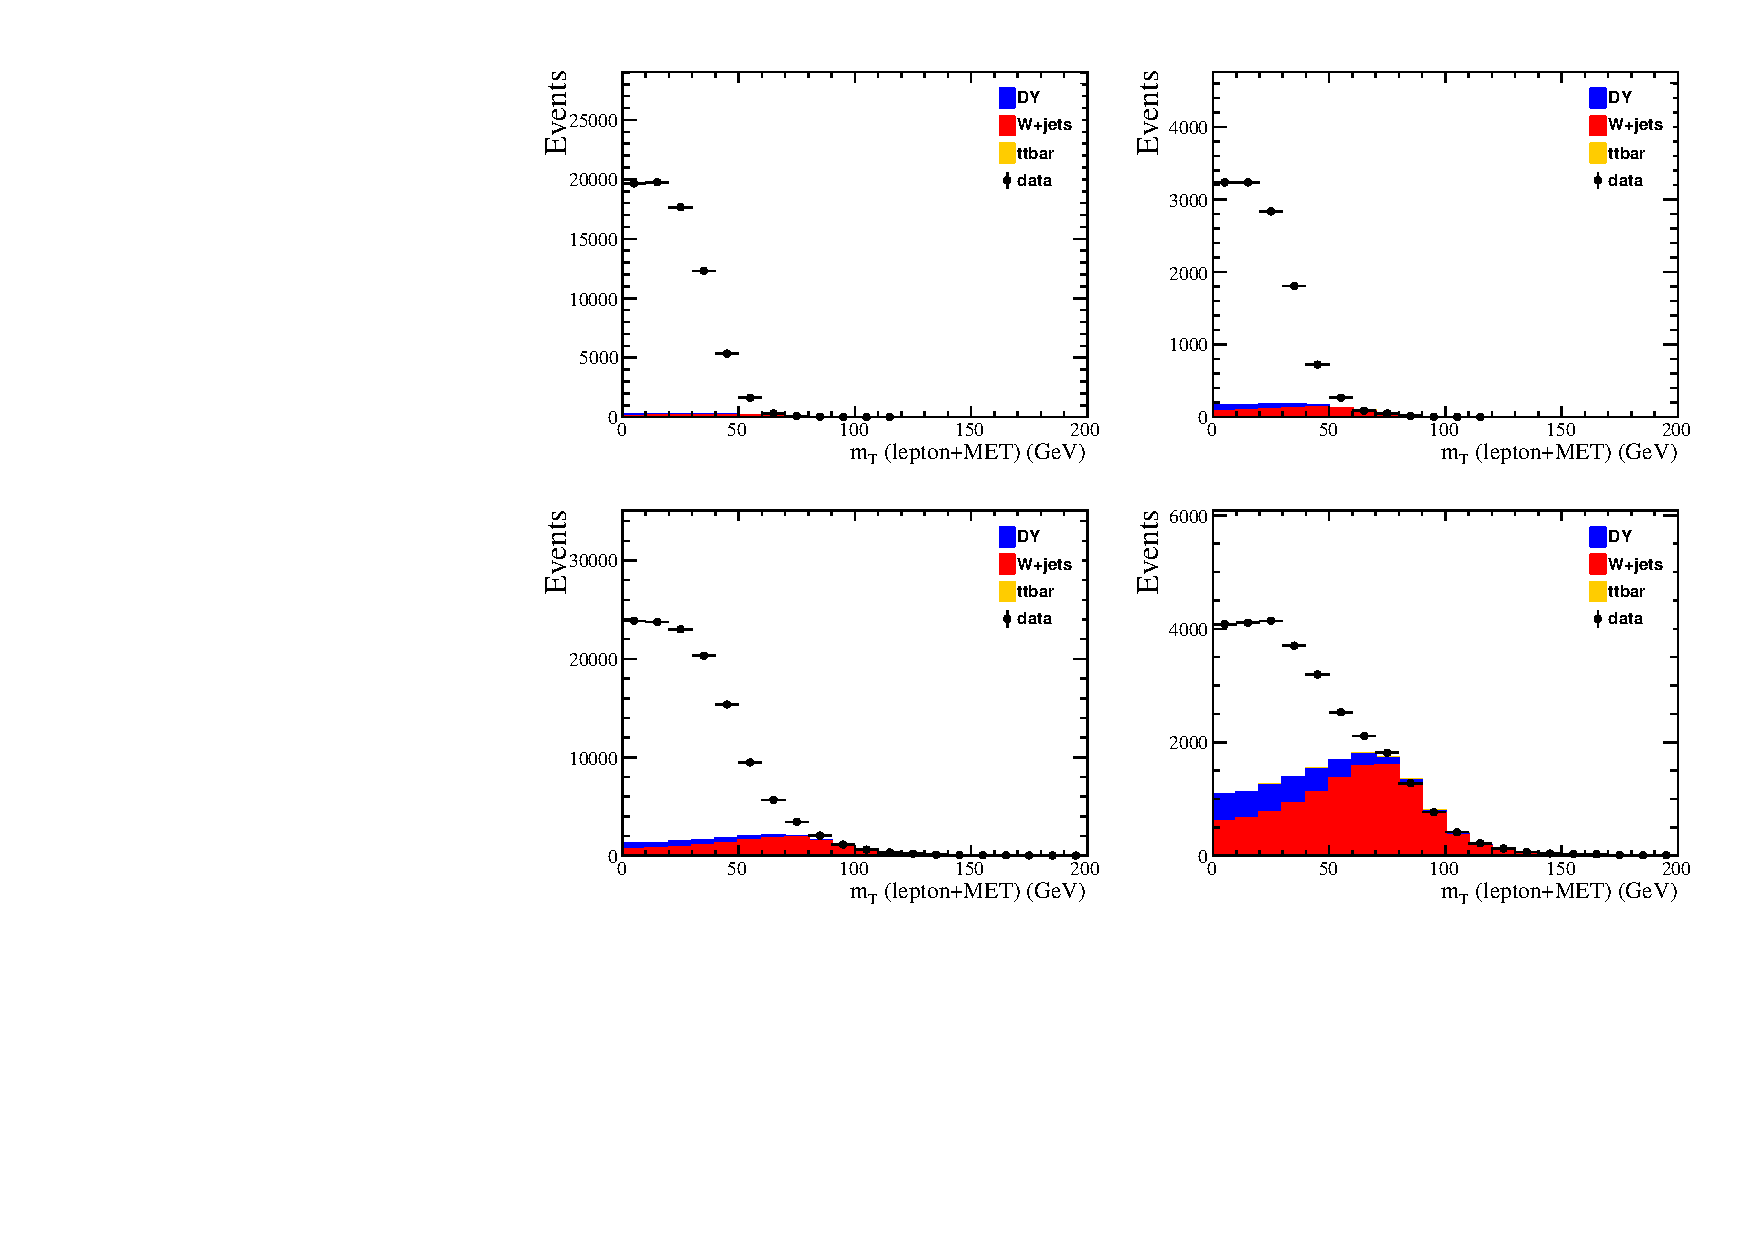
\includegraphics[width=.5\textwidth]{Figures/c5/FAKE/ele_mt.pdf}
\caption{$\MT$ distributions for electron . In the left column there
  are transverse mass distributions for \fo  (denominator) while in the
  right one for \ti  leptons (numerator). Two rows for the two electron triggers:
 Ele8 $\ptcone  \in  [10,18]$\GeV
  and Ele12 $\ptcone  > 18$\GeV.}
\label{fig:mt_fake_ele}
\end{figure}
}
\begin{figure}[h!]
\centering
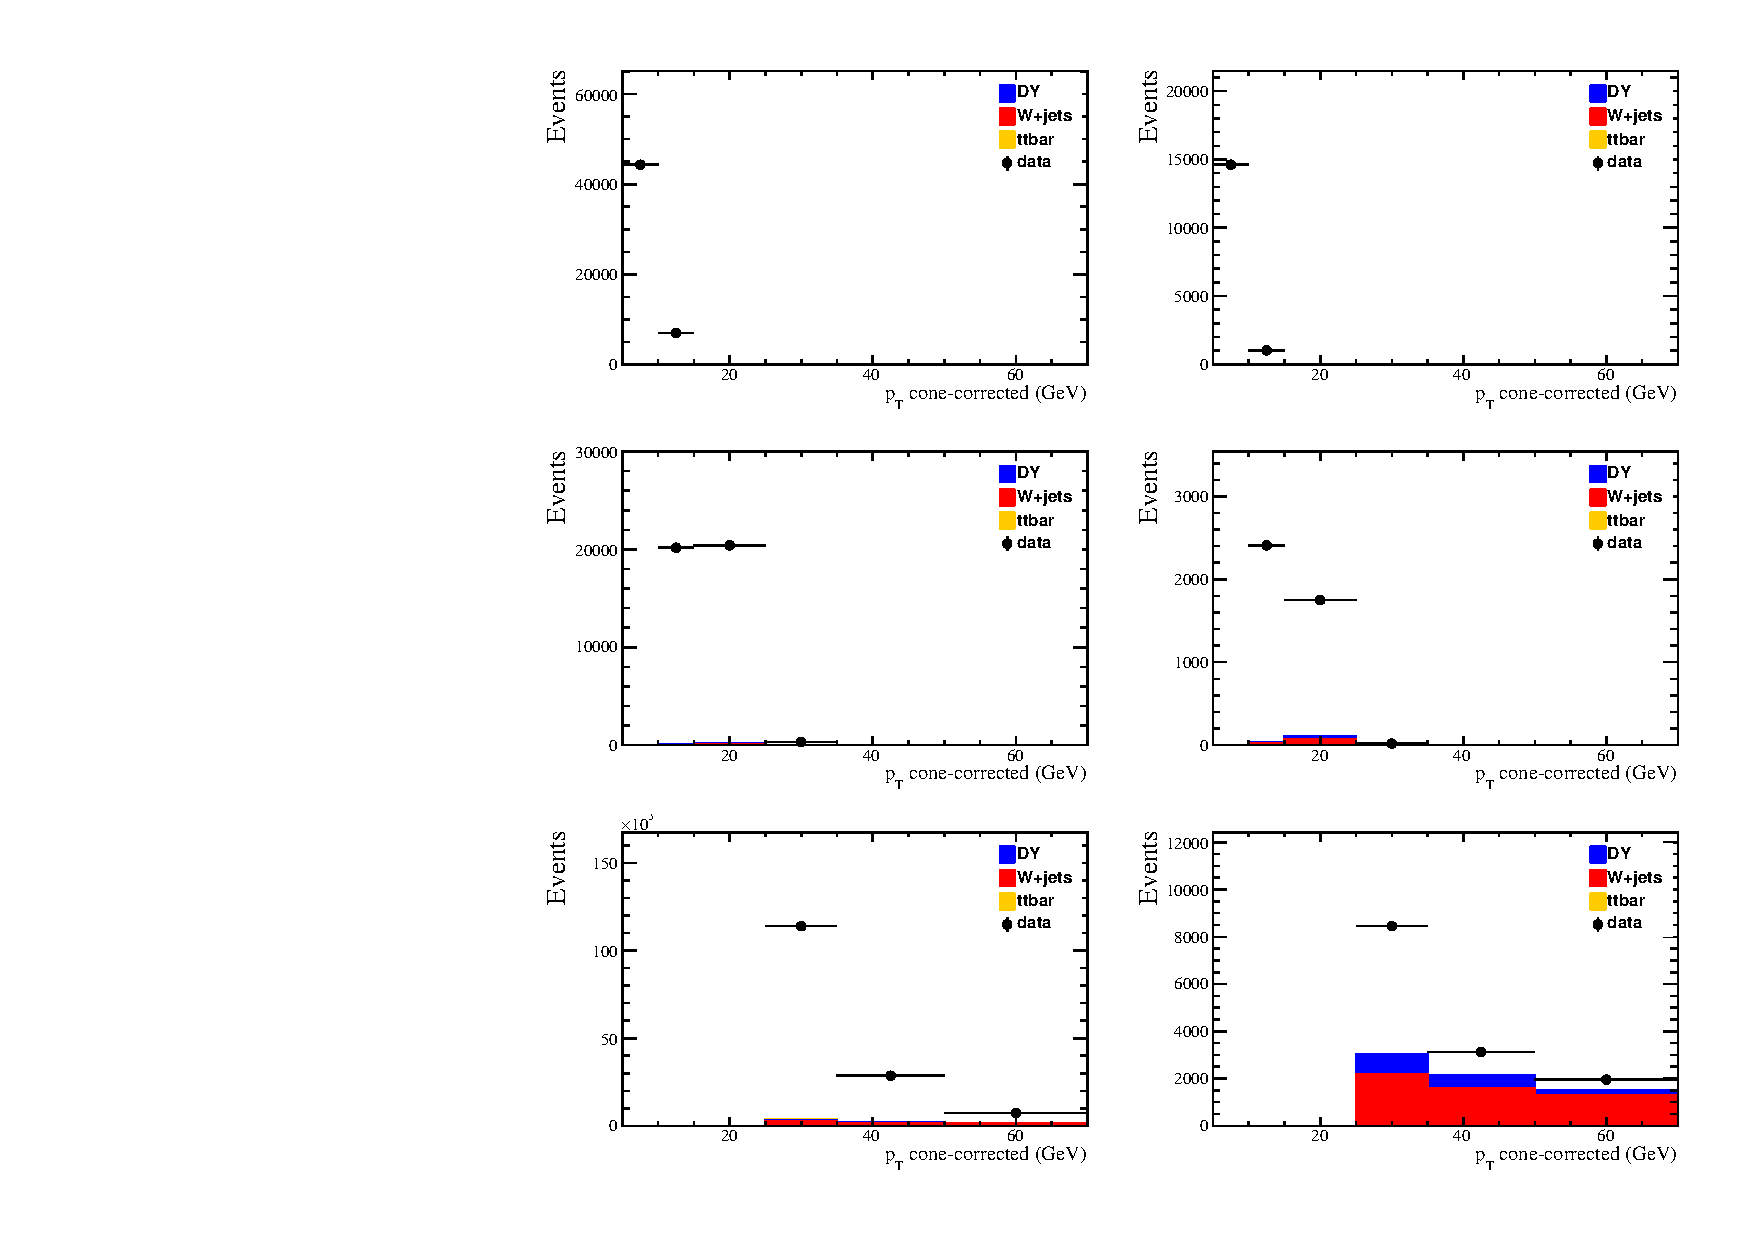
\includegraphics[width=.7\textwidth]{Figures/c5/FAKE/pt_cone_muon.pdf}
\caption{$\ptcone$ distributions, here labeled $\ptcone$-corrected,
  for muons. In the left column there are $\ptcone$ distributions for \fo  (denominator) while in the
  right one for \ti  leptons (numerator). Three
  rows for the three muon triggers: Mu3, $\ptcone \ \in \
  [5,12]$\GeV, Mu8 $\ptcone \ \in \
  [12,25.5]$\GeV and Mu17 $\ptcone \ > 25.5$\GeV.}
\label{fig:pt_fake_muon}
\end{figure}

\begin{figure}[h!]
\centering
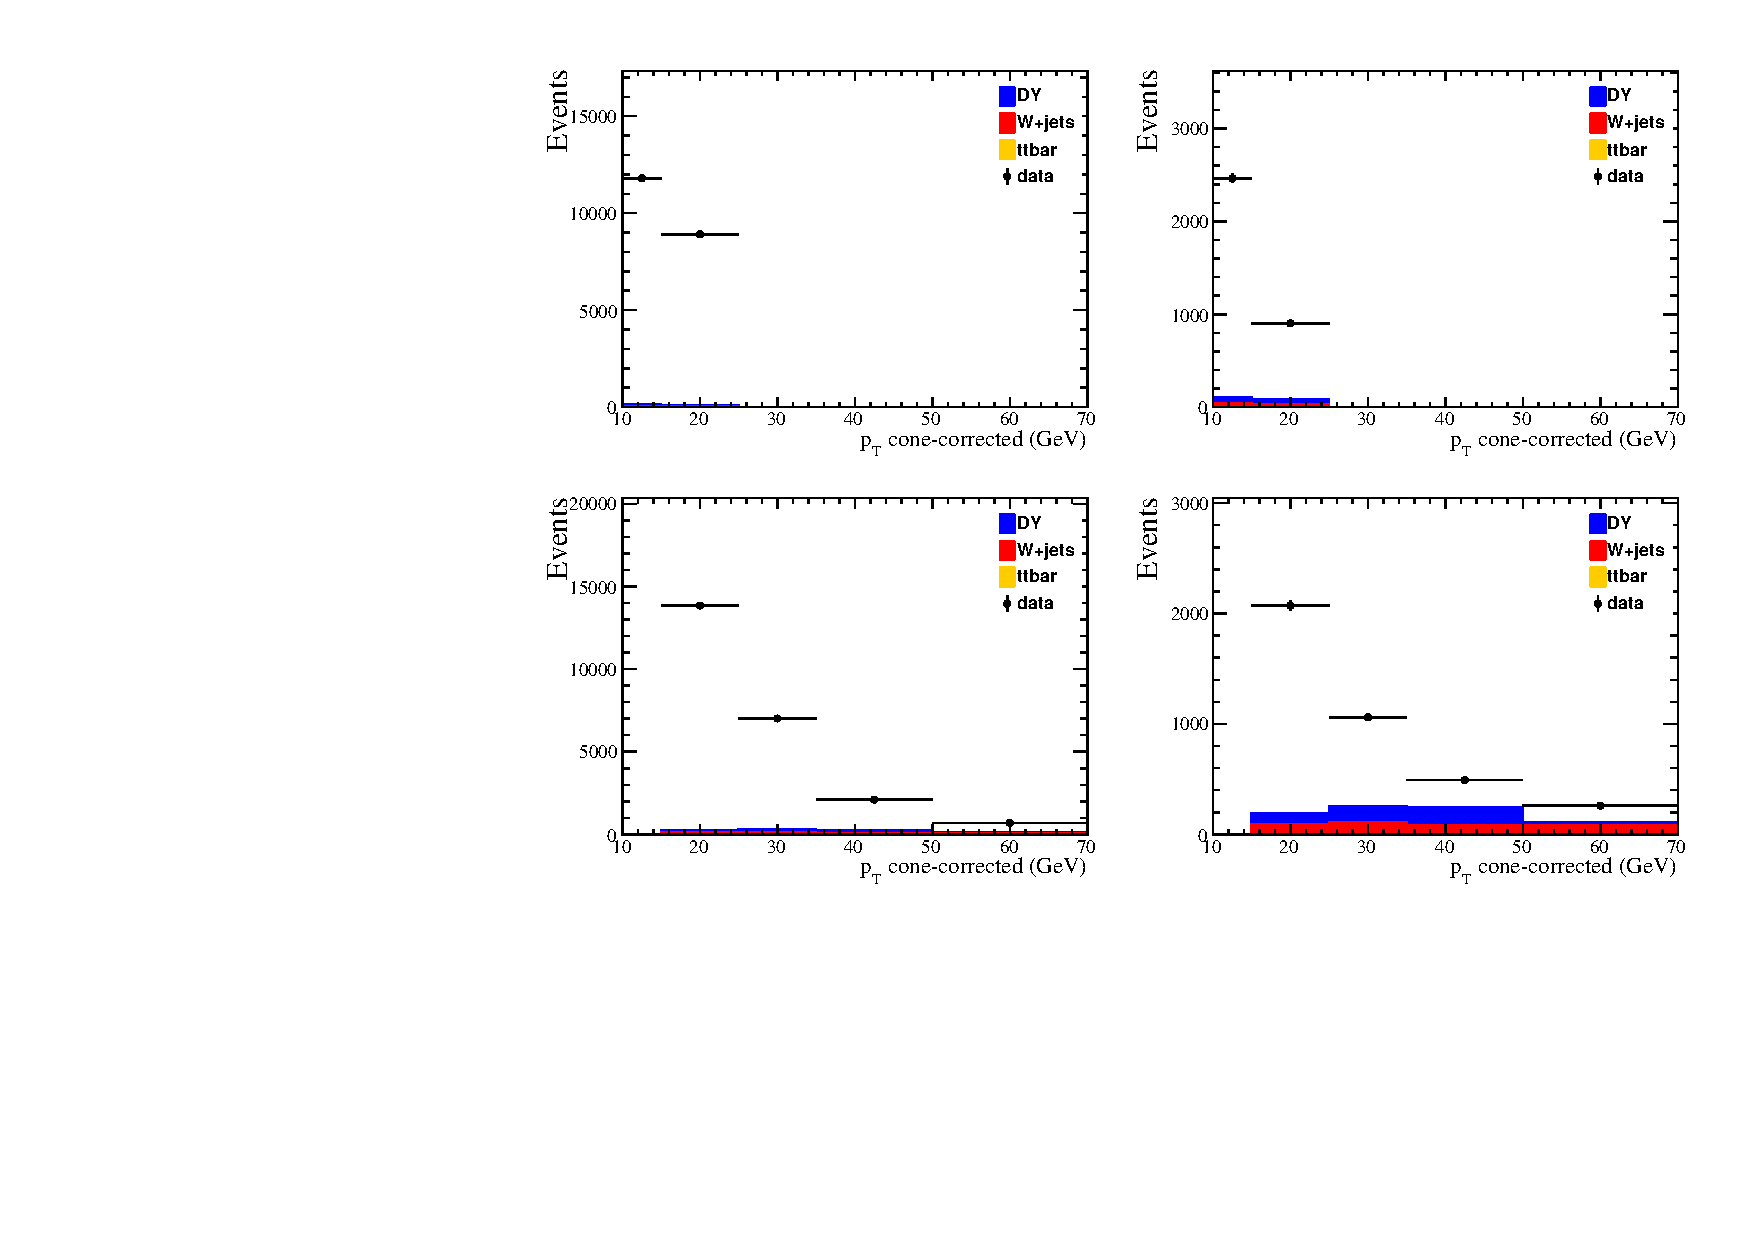
\includegraphics[width=.7\textwidth]{Figures/c5/FAKE/pt_cone_ele.pdf}
\caption{$\ptcone$ distributions, here labeled $\ptcone$-corrected,
  for electron. In the left column there are $\ptcone$ distributions
  for \fo  (denominator) while in the
  right one for \ti  leptons (numerator). Two
  rows for the two electron triggers: Ele8 $\ptcone \ \in \ [10,18]$\GeV
  and Ele12 $\ptcone \ > 18$\GeV.}
\label{fig:pt_fake_ele}
\end{figure}

In Figures~\ref{fig:pt_fake_muon} and ~\ref{fig:pt_fake_ele} 
the contribution of the prompt leptons in the measurement region is shown, after
the normalization. As we expected the majority of leptons from \PW and
\PZ production is association with a jet is located in the region with
high $\pt$ leptons. This is
reflected in the calculation of the \fr map.

\paragraph{\fr measured in MC}
We also measure the \fr in MC QCD di-jets and MC $\ttbar$ by
finding a nonprompt lepton by means of MC truth-matching. In
Figure~\ref{fig:comparison_muon} the comparisons between the fake rate
measured in data and in MC (QCD di-jets and $\ttbar$)  are
presented.\\
The data-MC comparison offers the possibility to verify and cross-check the
measurement done in data. The usage of the MC truth-information
guarantees the proper identification of the nonprompt leptons among
the leptons selected with the \fo and \ti  IDs. Hence the contamination
from prompt leptons in the denominator failing the \ti  selection is
none. Thus the discrepancies in Figure.~\ref{fig:comparison_muon} in the
bins at high \pt are due to the large EWK contamination. Then the last
bin is not used due to the sizable EWK contamination, leptons with \pt
larger than 40\GeV are predicted with \fr measured with leptons
with \pt $[35-50]$\GeV.\\
It is essential to point out that for this analysis the softest lepton (trailing) is typically the one the fails the \ti  selection and it is predicted using the \fr ratio measured in data. Thus, the fact that the last bin of the FR shown in Figure~\ref{fig:comparison_muon} is not used does not affect the analysis because there are no fake leptons at high \pt. 


\begin{figure}[h!]
\centering
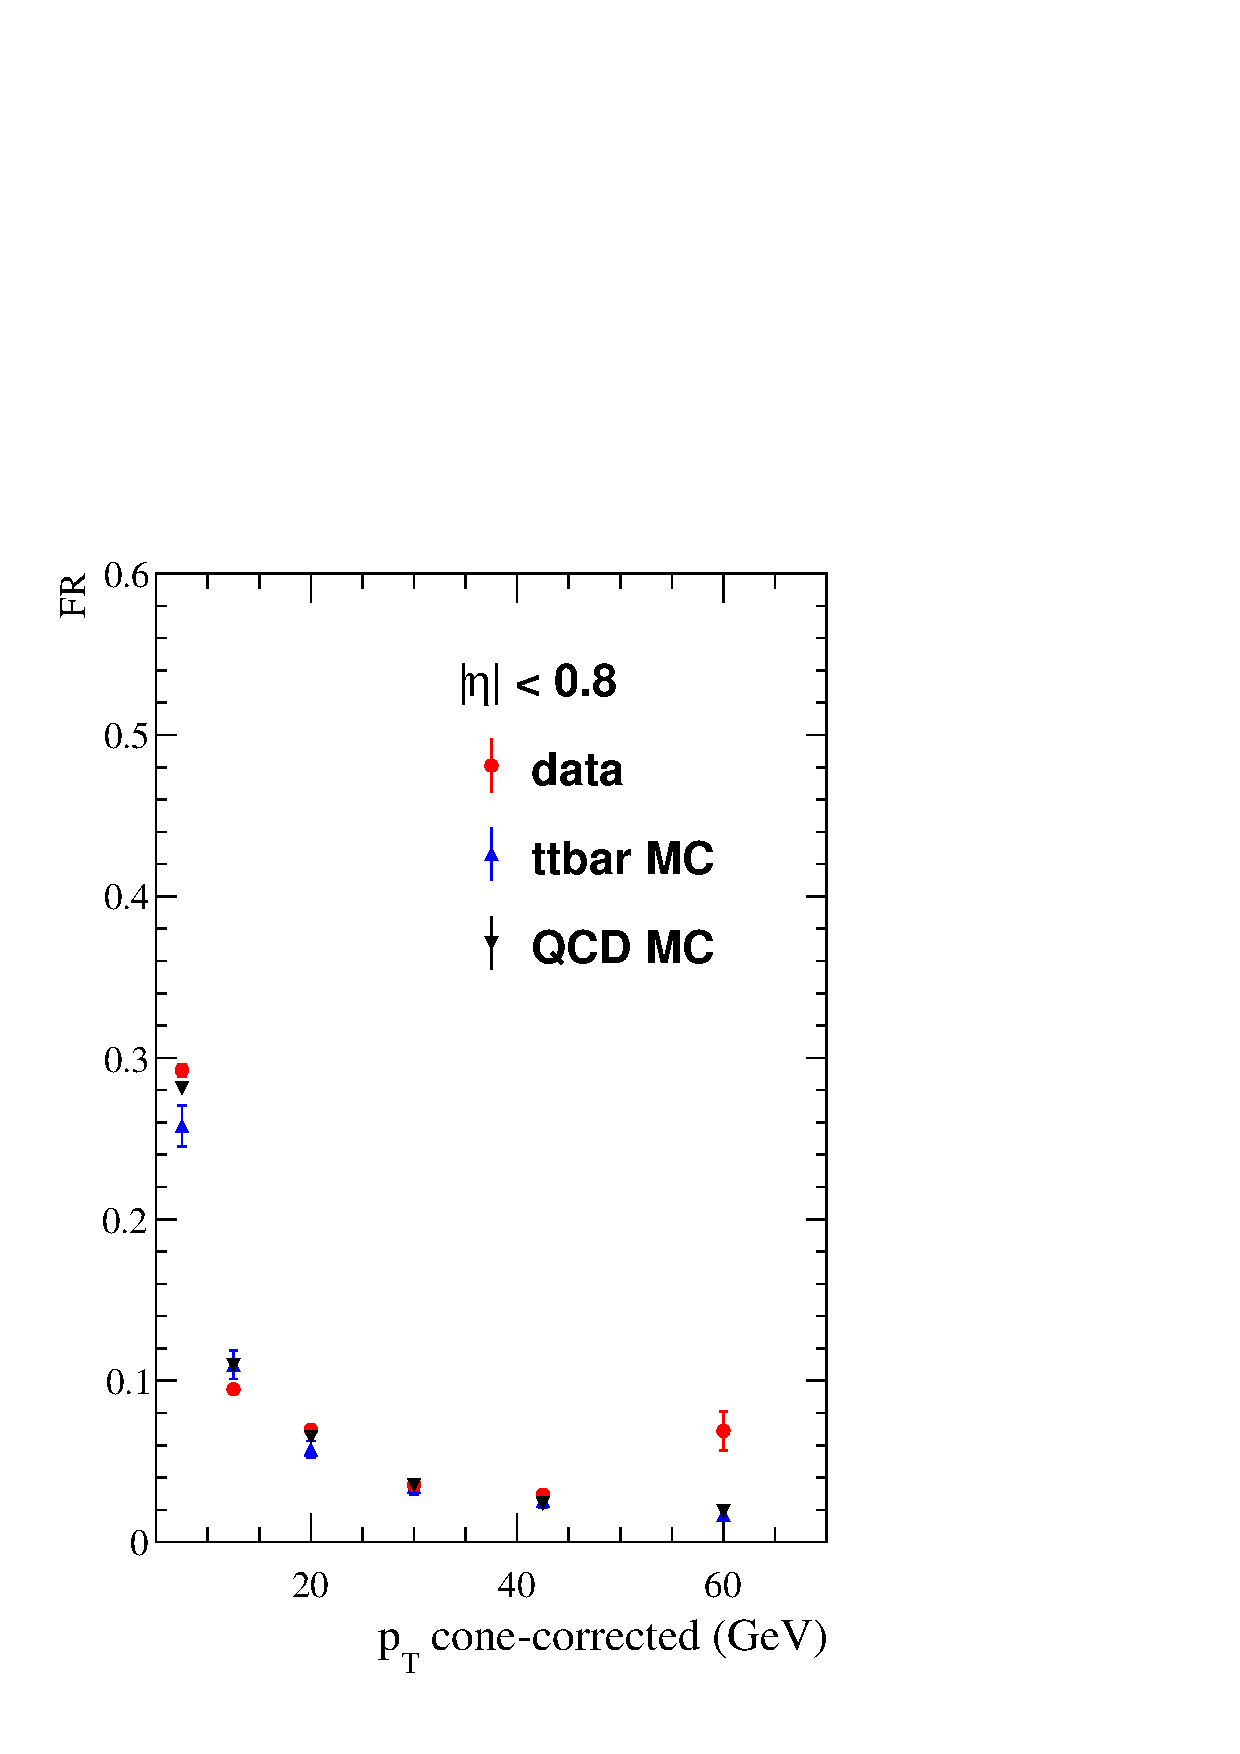
\includegraphics[width=.23\textwidth]{Figures/c5/FAKE/muon1.pdf}
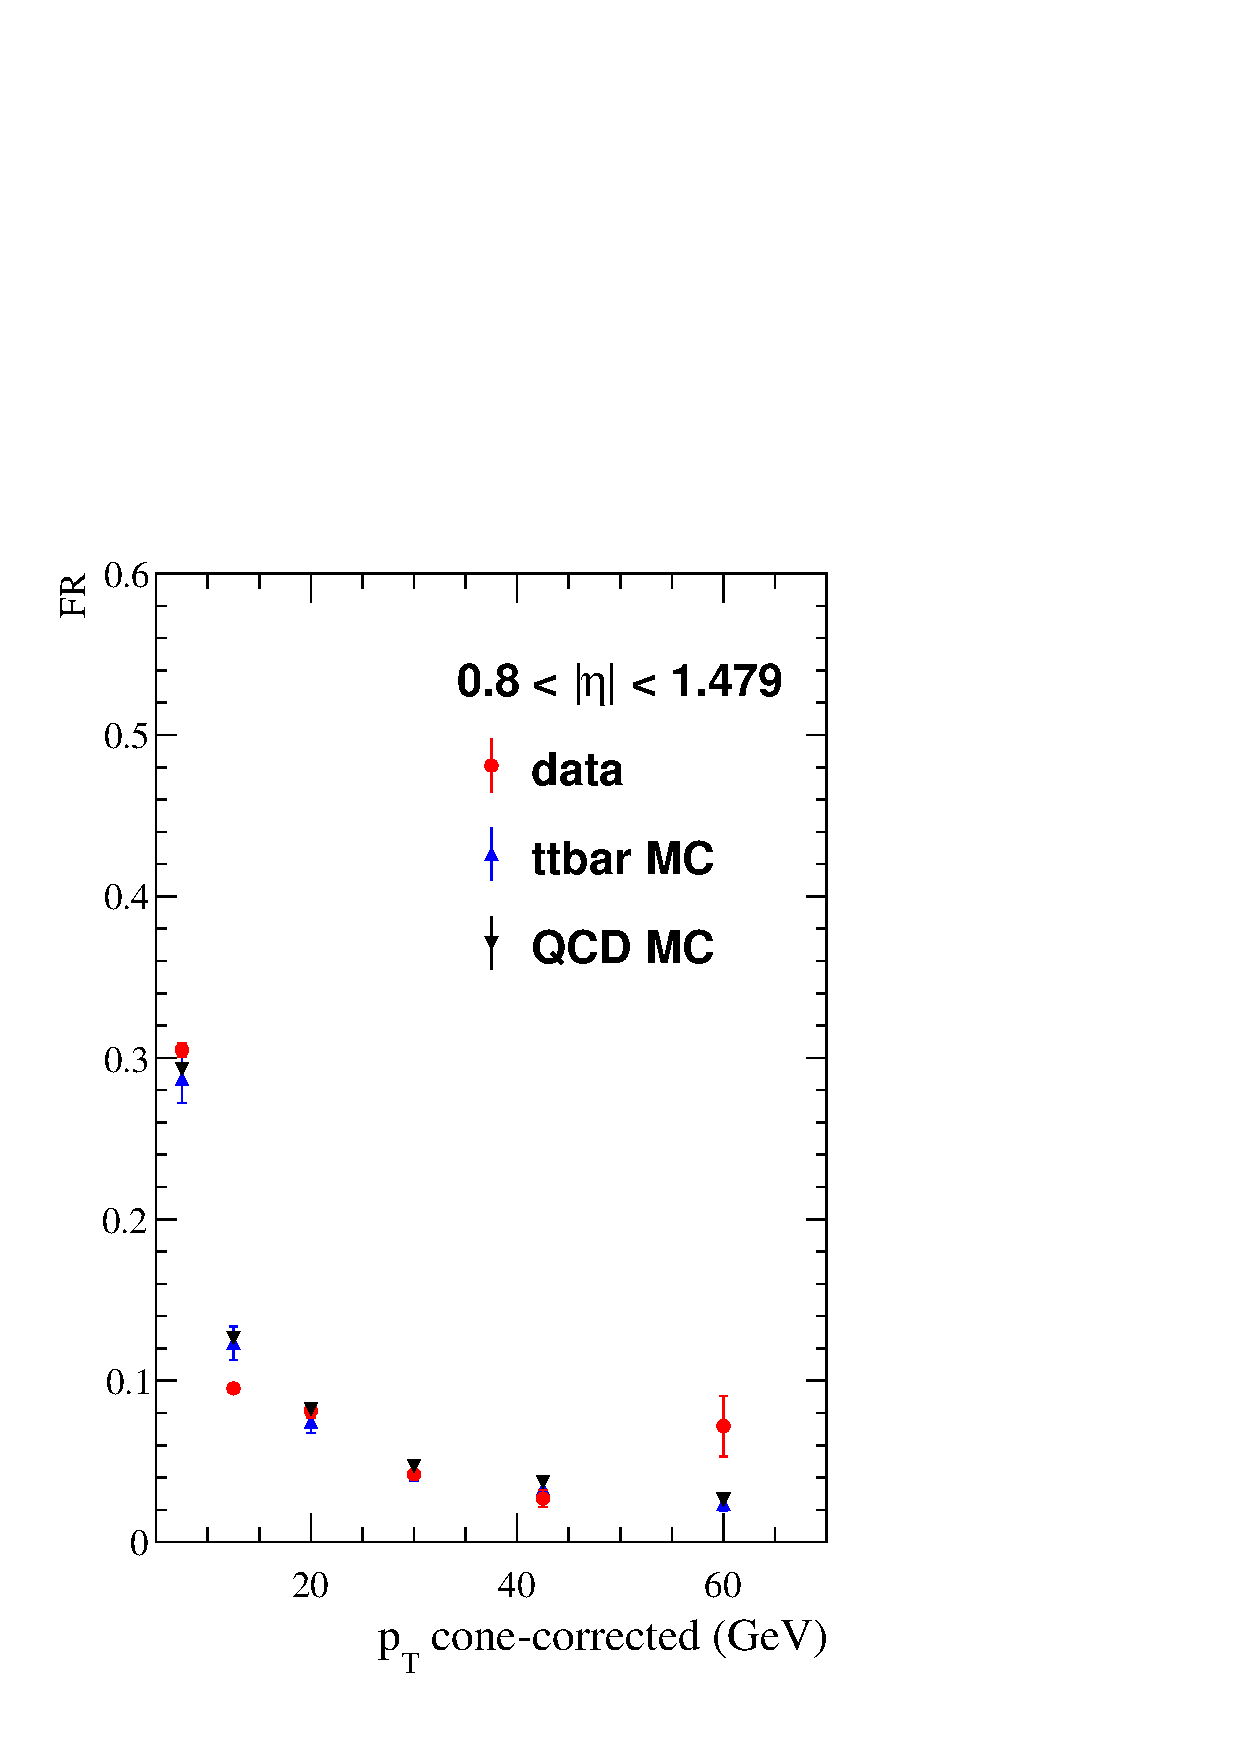
\includegraphics[width=.23\textwidth]{Figures/c5/FAKE/muon2.pdf}
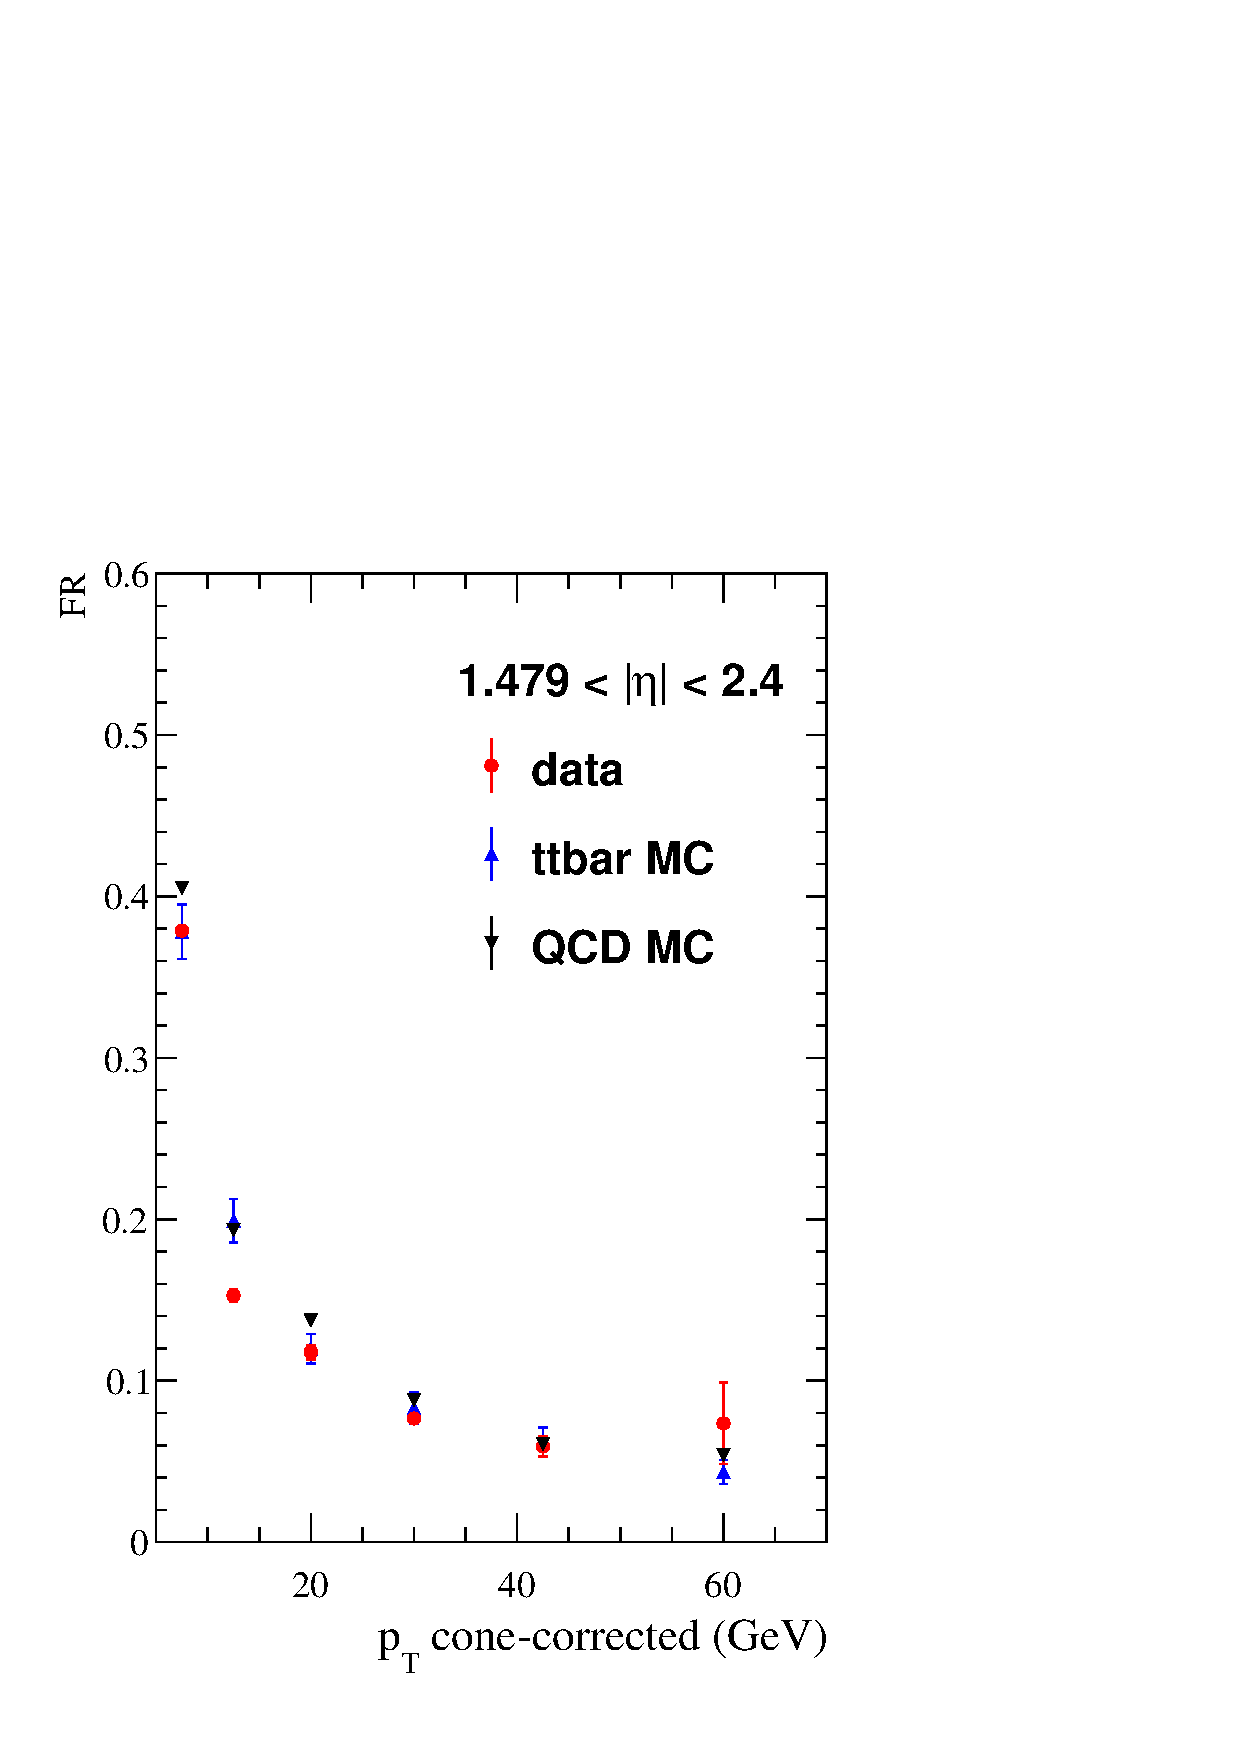
\includegraphics[width=.23\textwidth]{Figures/c5/FAKE/muon3.pdf}\\
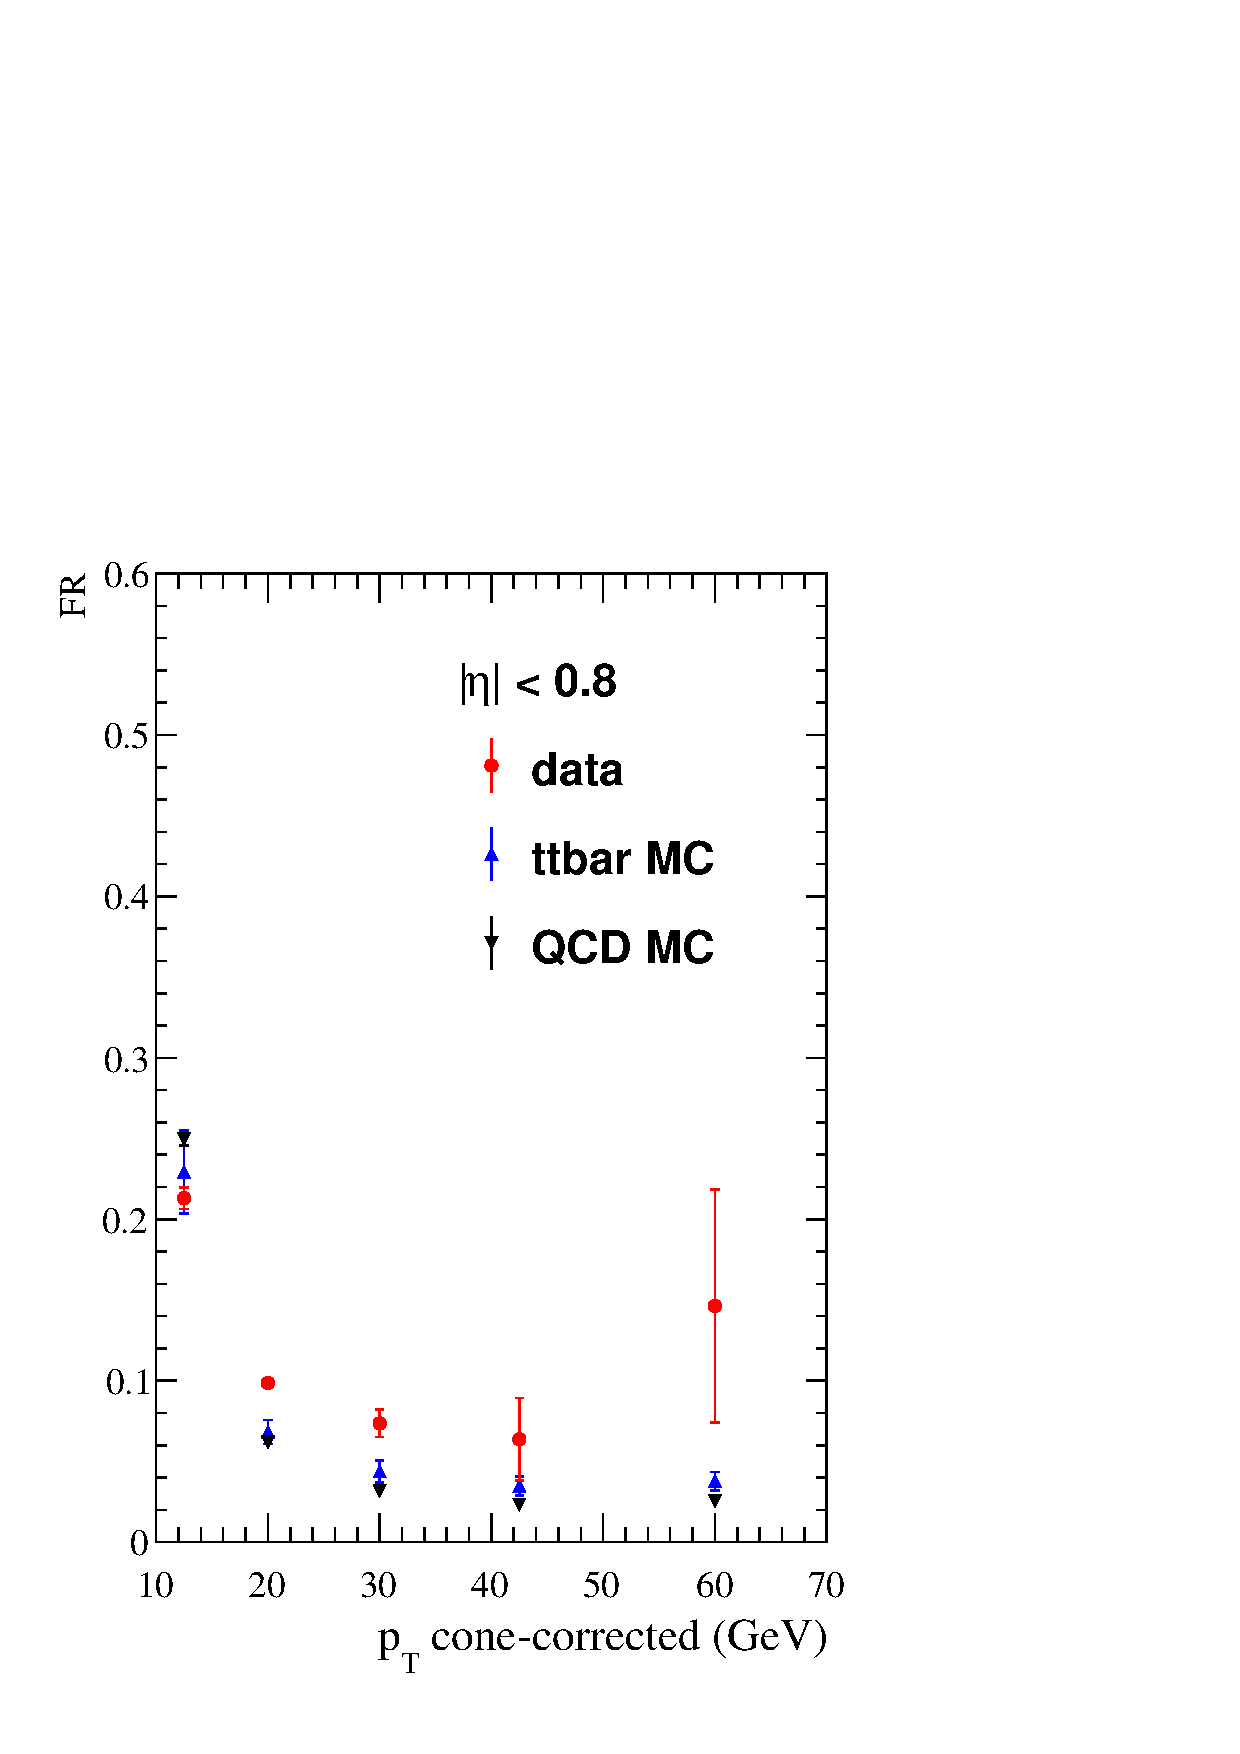
\includegraphics[width=.23\textwidth]{Figures/c5/FAKE/ele1.pdf}
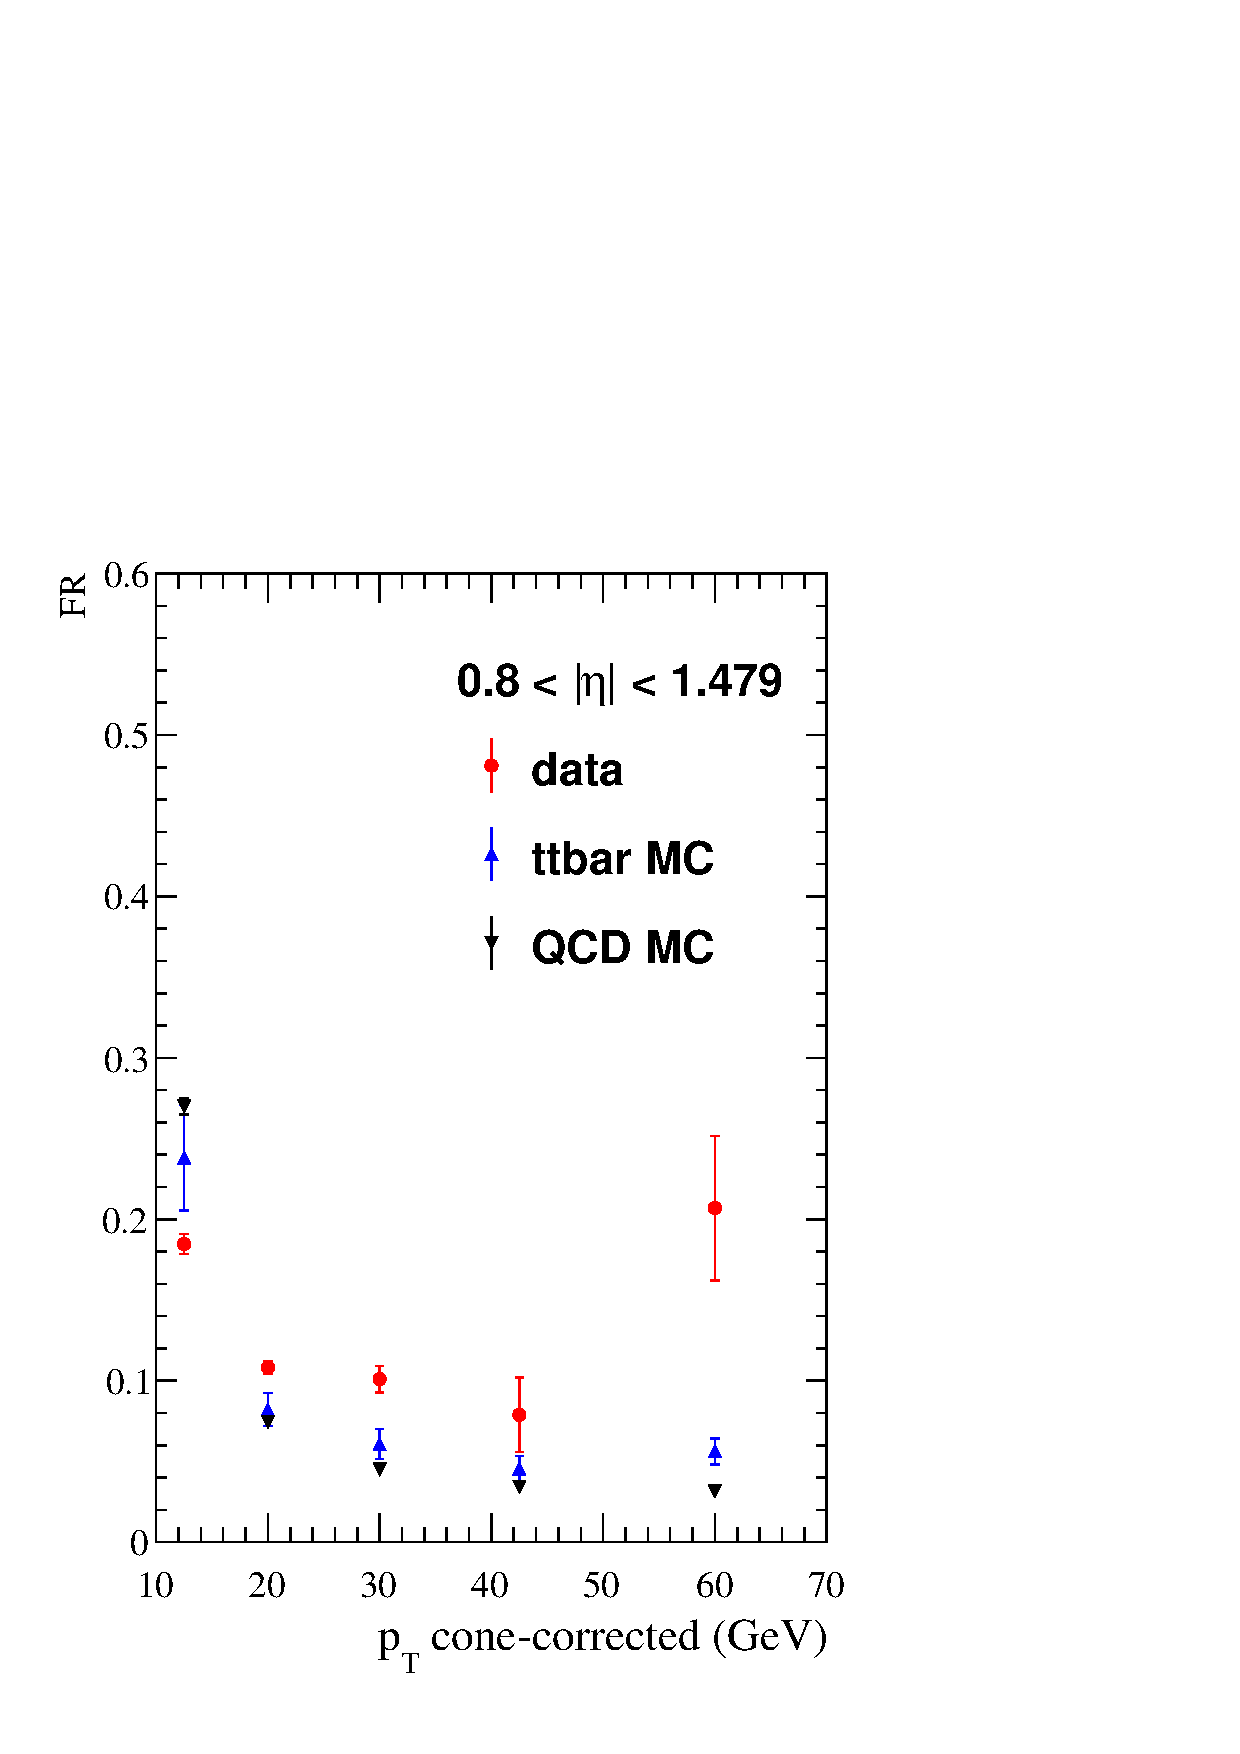
\includegraphics[width=.23\textwidth]{Figures/c5/FAKE/ele2.pdf}
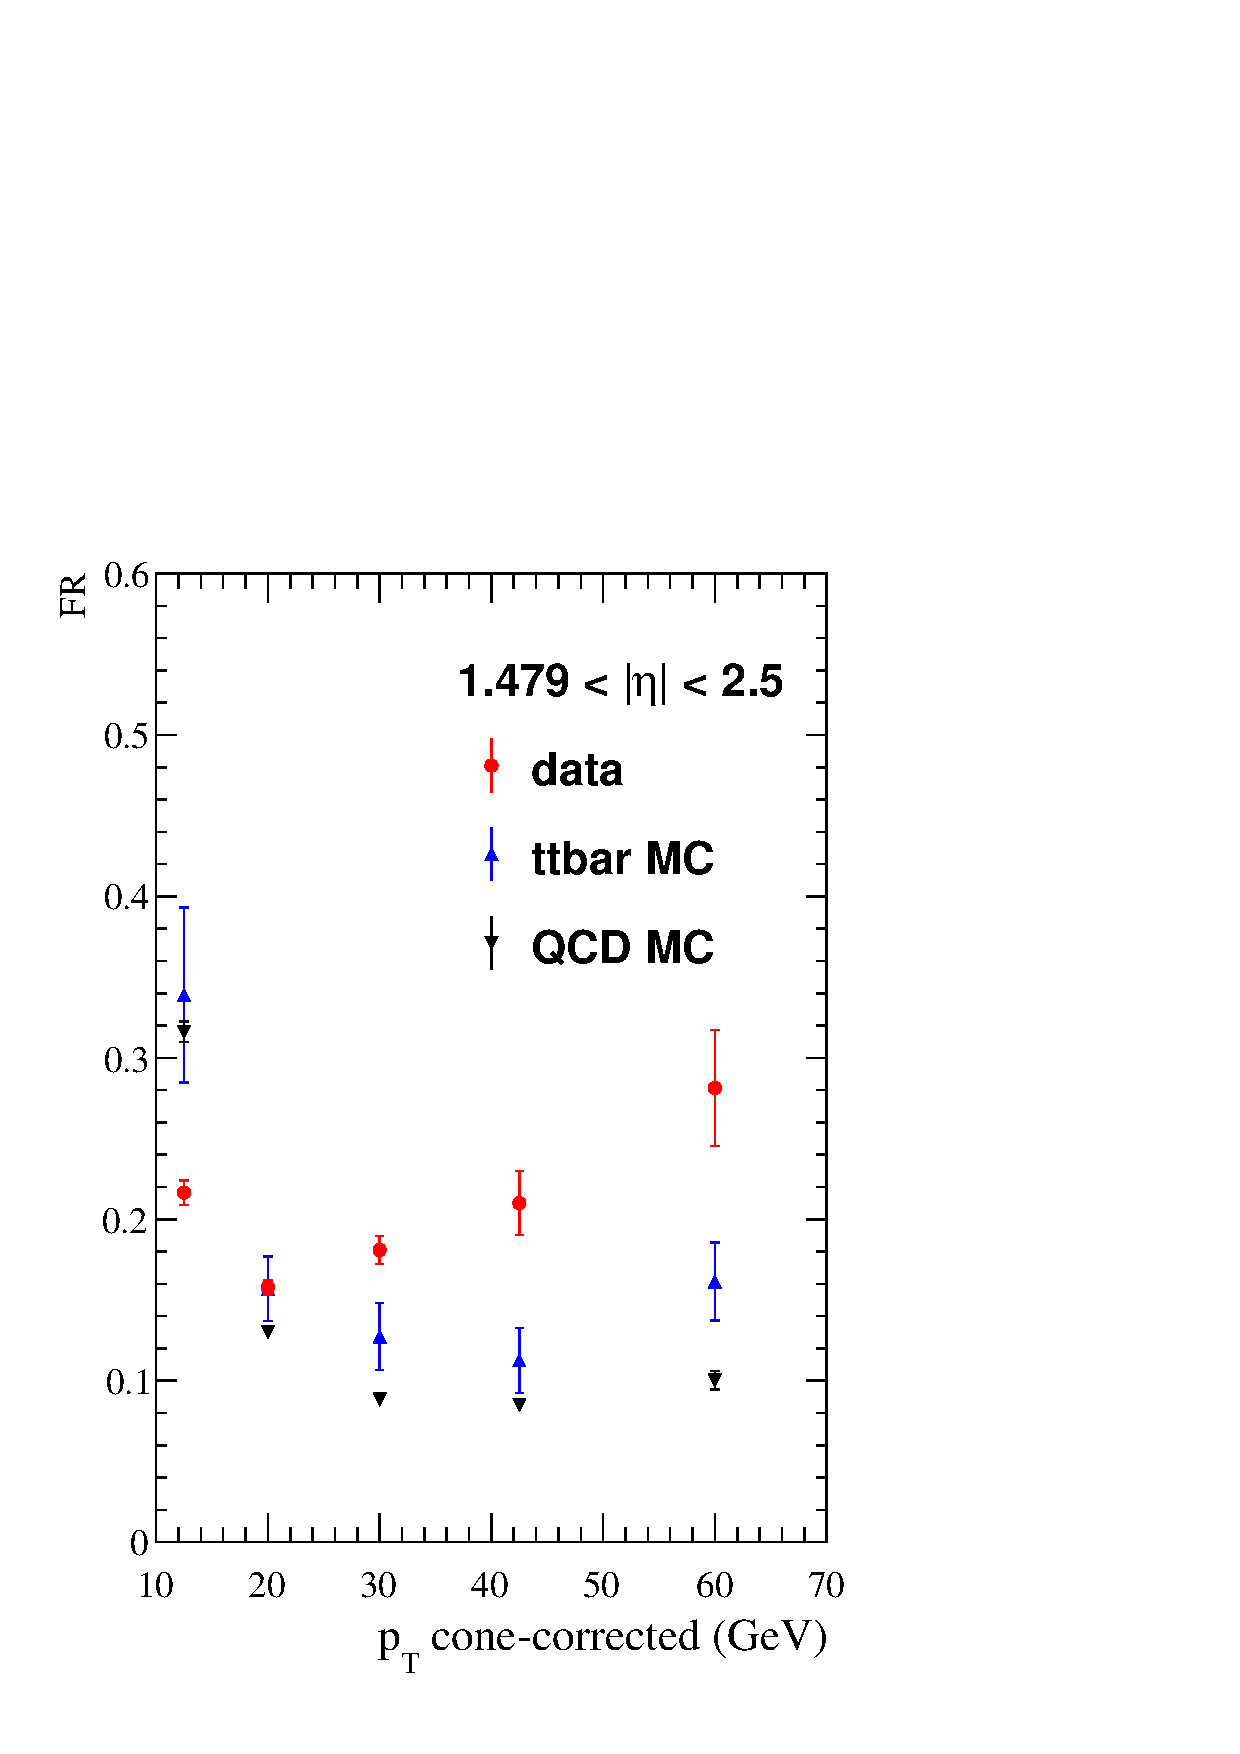
\includegraphics[width=.23\textwidth]{Figures/c5/FAKE/ele3.pdf}
\caption{\fr values for muons (top) and electron (bottom), calculated in data (red), QCD MC (black) and $\ttbar$ MC(blue).The last bin is not used due to the large EWK contamination, leptons with \pt larger than 40\GeV are predicted with FR at the bin $[35-50]$\GeV.}
\label{fig:comparison_muon}
\end{figure}


\subsubsection{\fr application}
We define the application region requiring at least one of the three
selected leptons to fail the \ti  lepton definition. In the signal region, we estimate the contribution by expressing the yields of events where $l$ leptons pass the full selection, and $n \ - \ l$ fail it. In this way the background prediction is obtained by weighting the events in the application region according to:
\begin{itemize}
\setlength\itemsep{-0.2em}
\item if the event is $T_{1}T_{2}L_{3}$, i.e. only one fails, it is weighted by $f_{3}/(1-f_{3})$
\item if the event is $T_{1}L_{2}L_{3}$, i.e. two fail, it is weighted
  by $- (f_{2} \ f_{3})/(1-f_{2})(1-f_{3})$
\item if the event is $L_{1}L_{2}L_{3}$, i.e. all fail, it is weighted by $(f_{1} \ f_{2} \ f_{3})/(1-f_{1})(1-f_{2})(1-f_{3})$
\end{itemize}
where $f_{i}$ is the \fr evaluated on the \ptcone and $\eta$
of the failing lepton.\\


\subsubsection{Validation of the \ttol method in simulation, \ttbar MC }
Closure tests are necessary in order to test if we are able to predict
the nonprompt background after the event selection requirements.

\begin{figure}[h!]
\noindent
\makebox[\textwidth]{
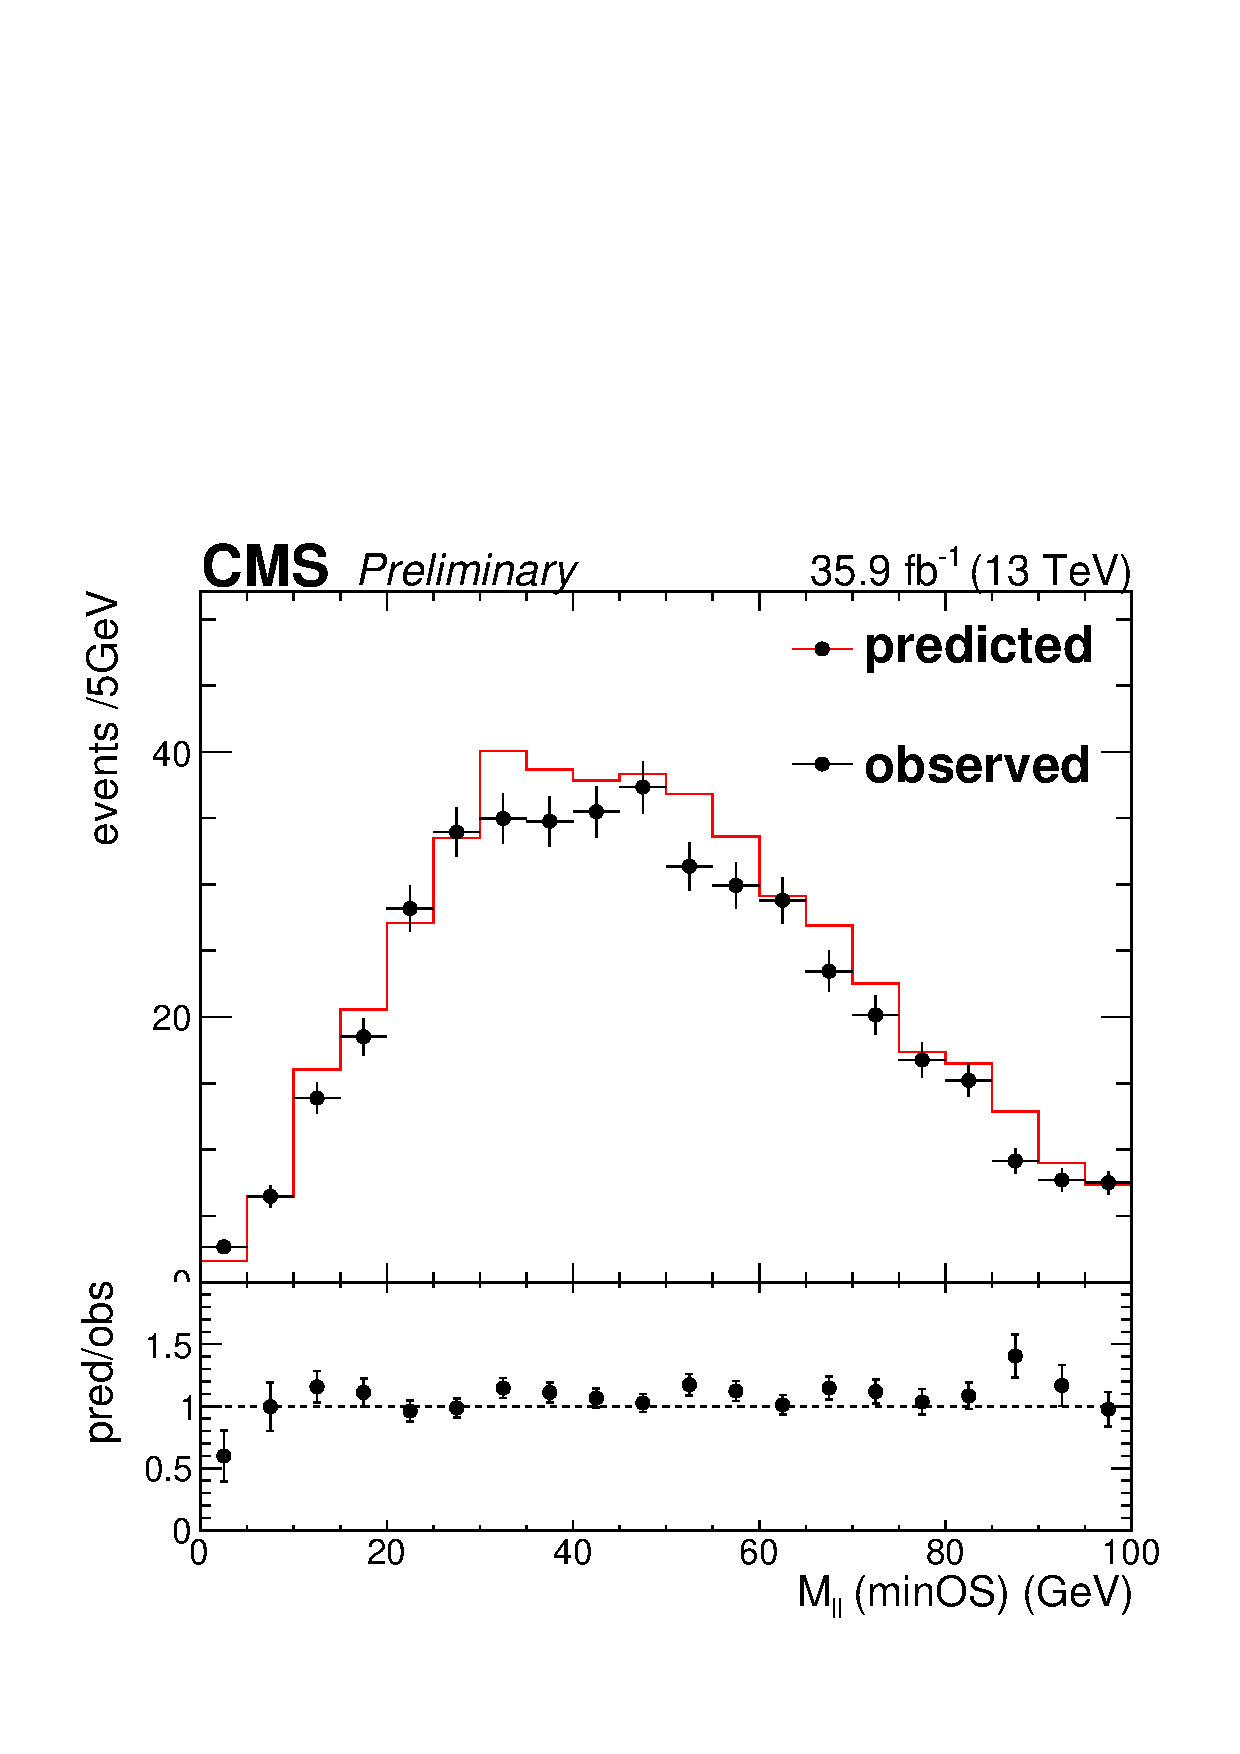
\includegraphics[width=.33\textwidth]{Figures/c5/FAKE/e_closuresMll.pdf}
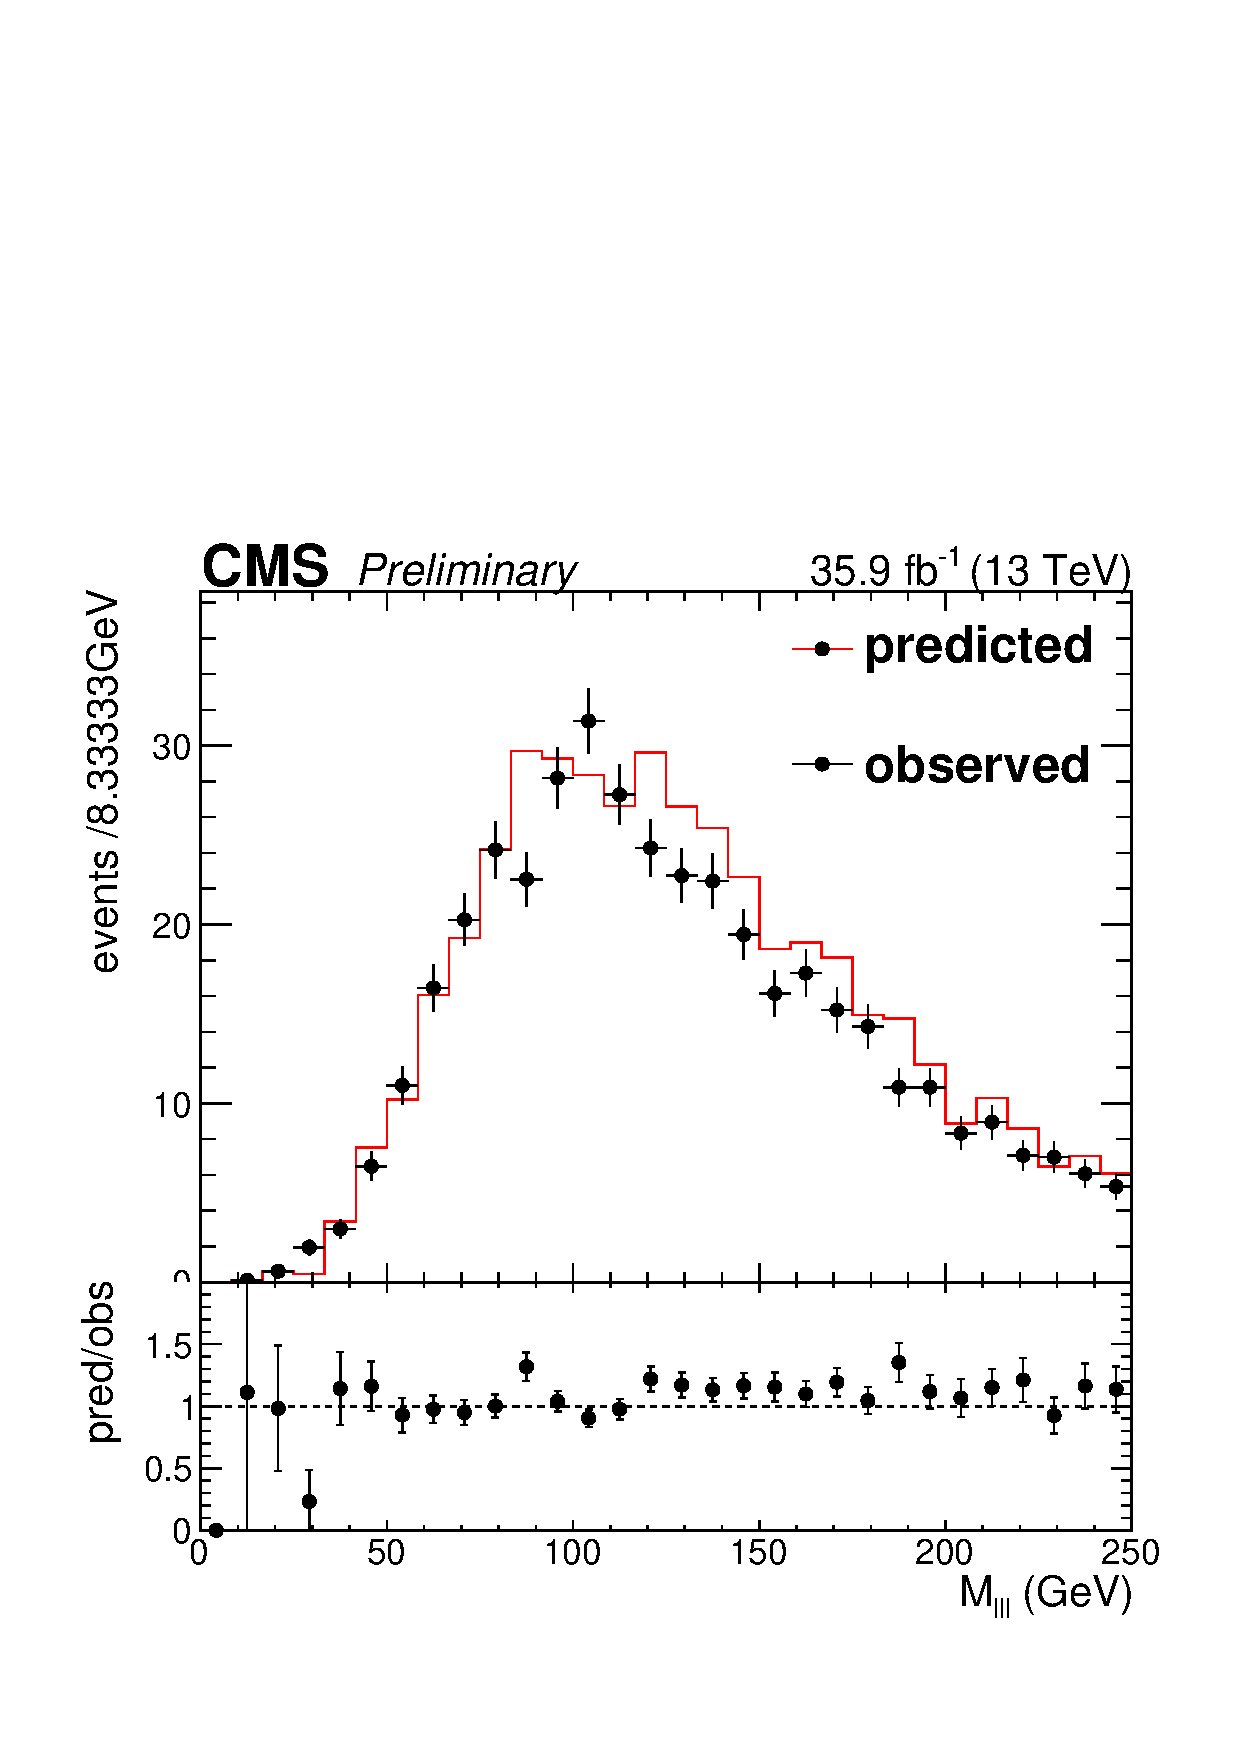
\includegraphics[width=.33\textwidth]{Figures/c5/FAKE/e_closuresMlll.pdf}}\\
\makebox[\textwidth]{
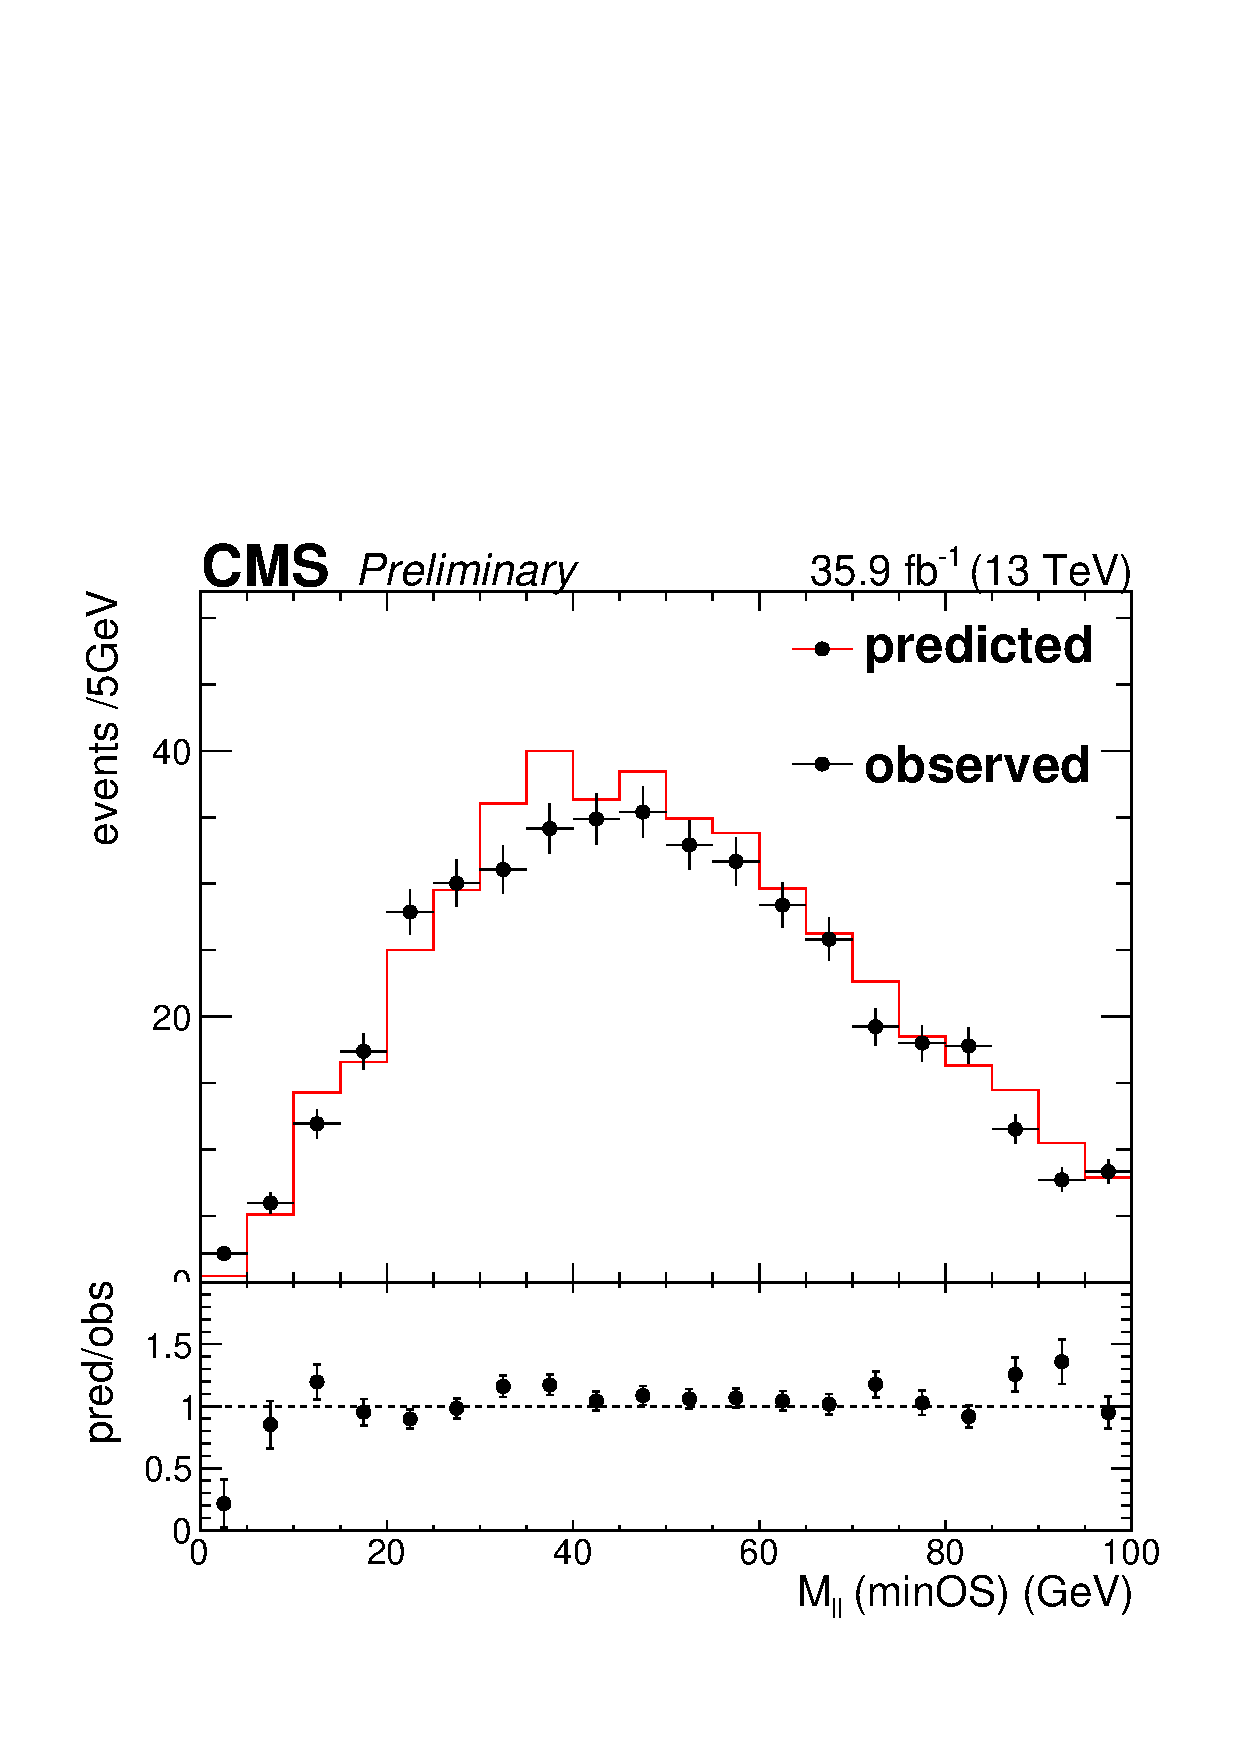
\includegraphics[width=.33\textwidth]{Figures/c5/FAKE/mu_closuresMll.pdf}
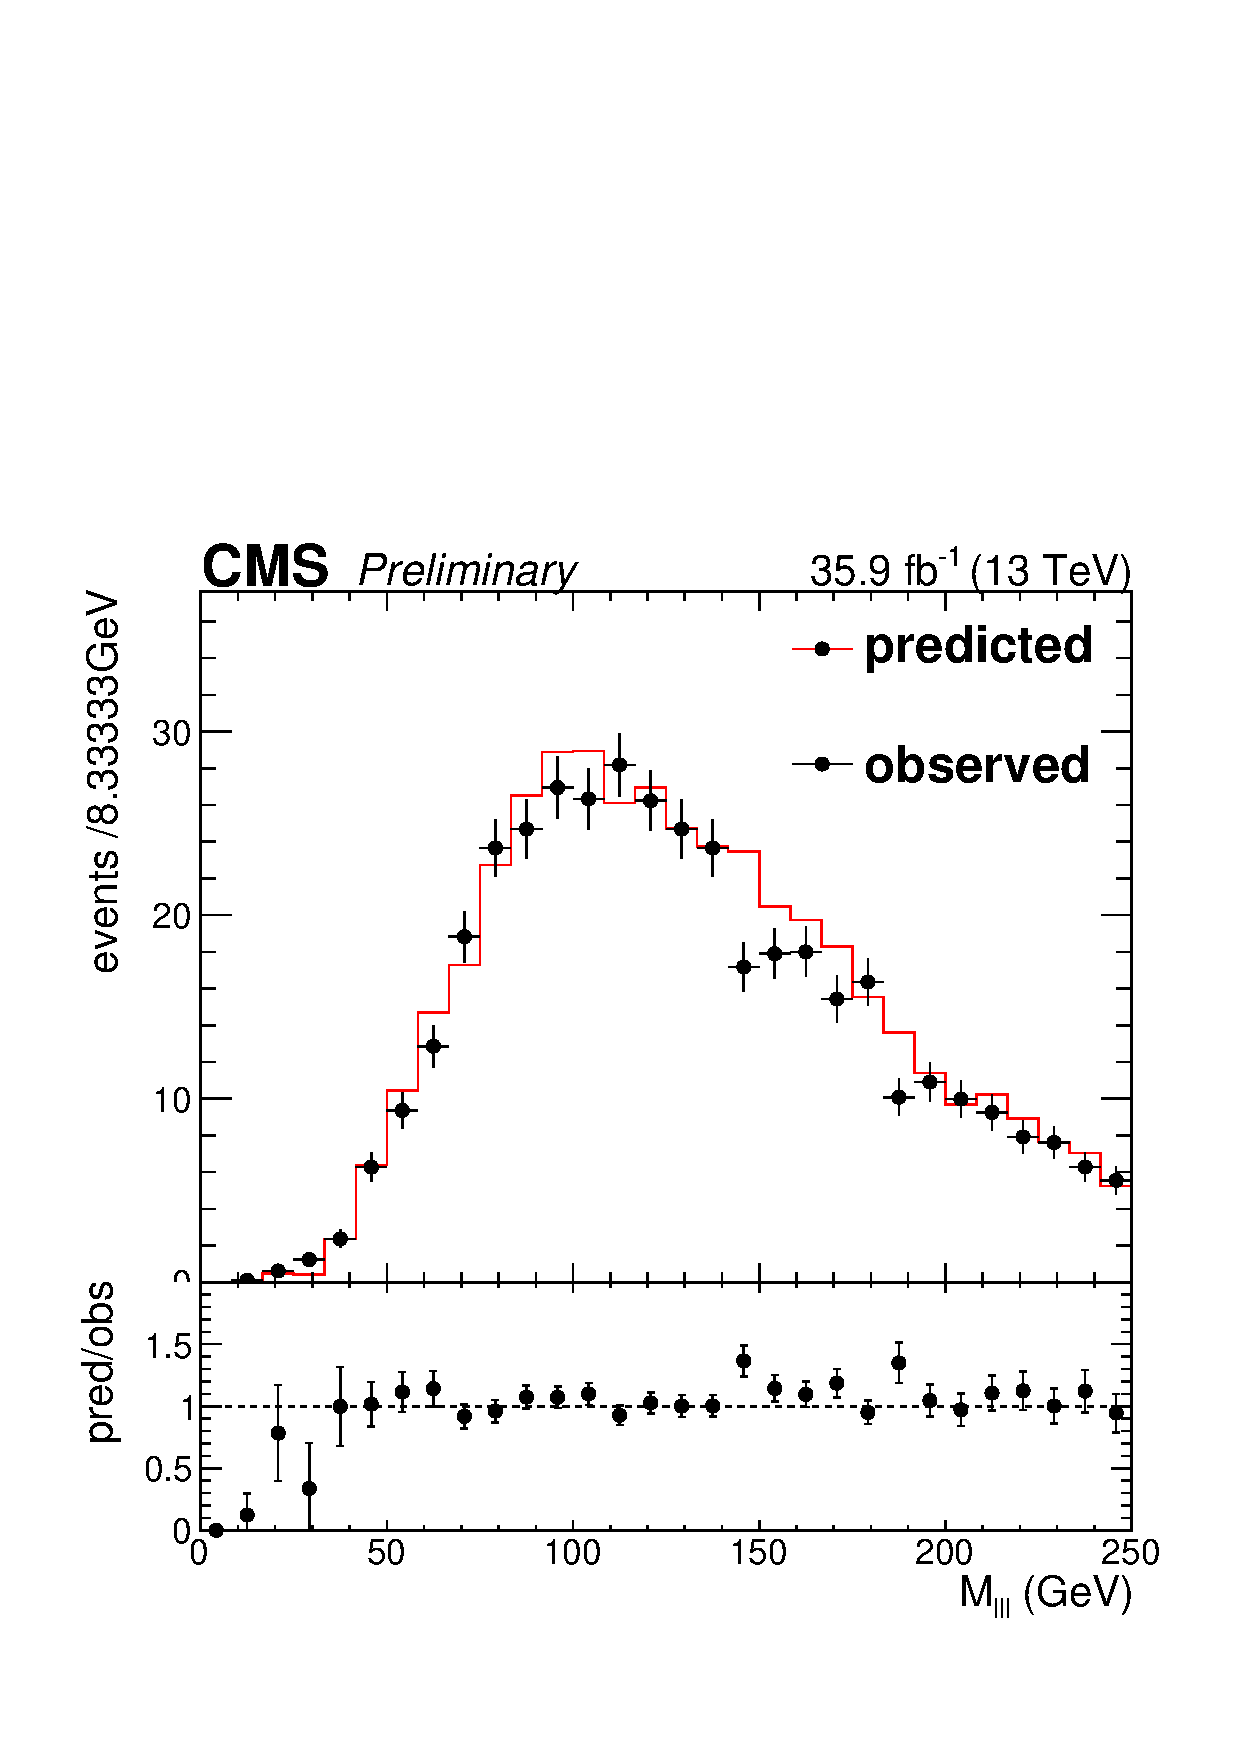
\includegraphics[width=.33\textwidth]{Figures/c5/FAKE/mu_closuresMlll.pdf}}
\caption{Closure test on $\ttbar$ for electrons (top) and for muons
  (bottom) with the \fr extracted from nonprompt leptons in QCD MC. Red lines are the predicted nonprompt $\ttbar$ events, black dots the observed number of nonprompt $\ttbar$ events using MC-truth information.}
\label{fig:closures2_ele}
\end{figure}
The \fr extracted from nonprompt leptons in QCD MC events is
used in the application region to estimate the nonprompt $\ttbar$
events in the signal region. Then we compare the observed number of
nonprompt $\ttbar$ events using MC-truth information. The results of
these tests in 3 lepton events are shown in the following
Figure~\ref{fig:closures2_ele}. The two variables which are shown are
the \mmin and \mlll already described and motivated in
Section~\ref{sec:analisi}.
As previously explained, the events are selected and divided in
categories according to the values of \mmin and \mlll; thus it is
mandatory having good understanding and control on the predictions for
these specific distributions which are used for the final results. \\
The plots in Figure~\ref{fig:closures2_ele} present excellent
agreement between predictions and observations with discrepancies 
smaller than 30\%.


\subsection{Nonprompt background validation}
In addition to the validation done with MC closure tests, we also want
to test it in data in two specific control regions: Drell-Yan
enriched and \ttbar enriched CR.
\paragraph{Drell-Yan enriched
  control region:} 
The major background contribution in the low mass region comes from Drell-Yan events in which a third lepton is a
nonprompt lepton. Thus, we define a control region requiring an OSSF pair with a mass within 15\GeV of that of the Z boson, and with \ptmiss $< 30$\GeV and $\MT < 30$\GeV . The latter
cuts largely remove the contamination from WZ in this control
region. The background prediction is then compared with data, and an excellent match is found, as shown in Figure~\ref{fig:npvalidation}. 
\begin{figure}[h!]
\centering
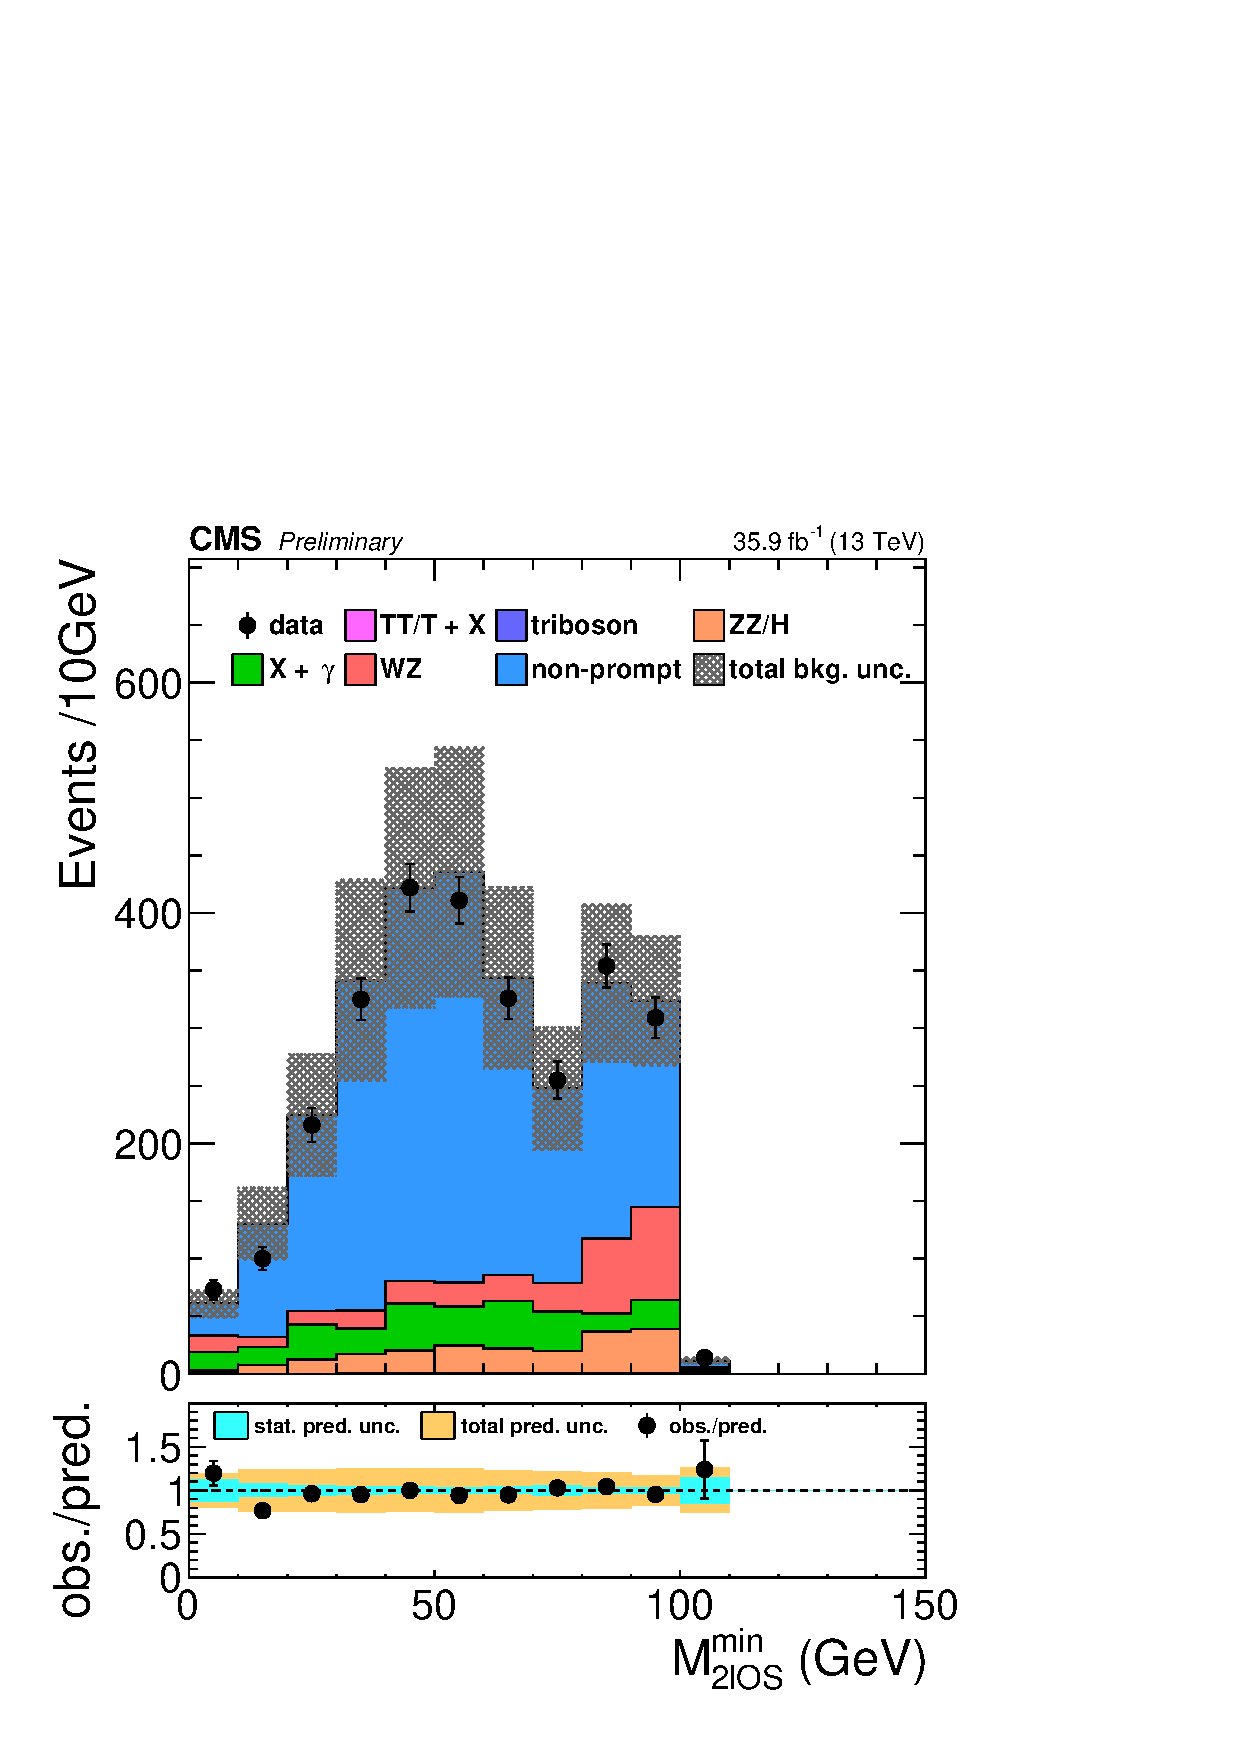
\includegraphics[width=.30\textwidth]{Figures/c5/DYCR/inclusive/minMos_DY.pdf}
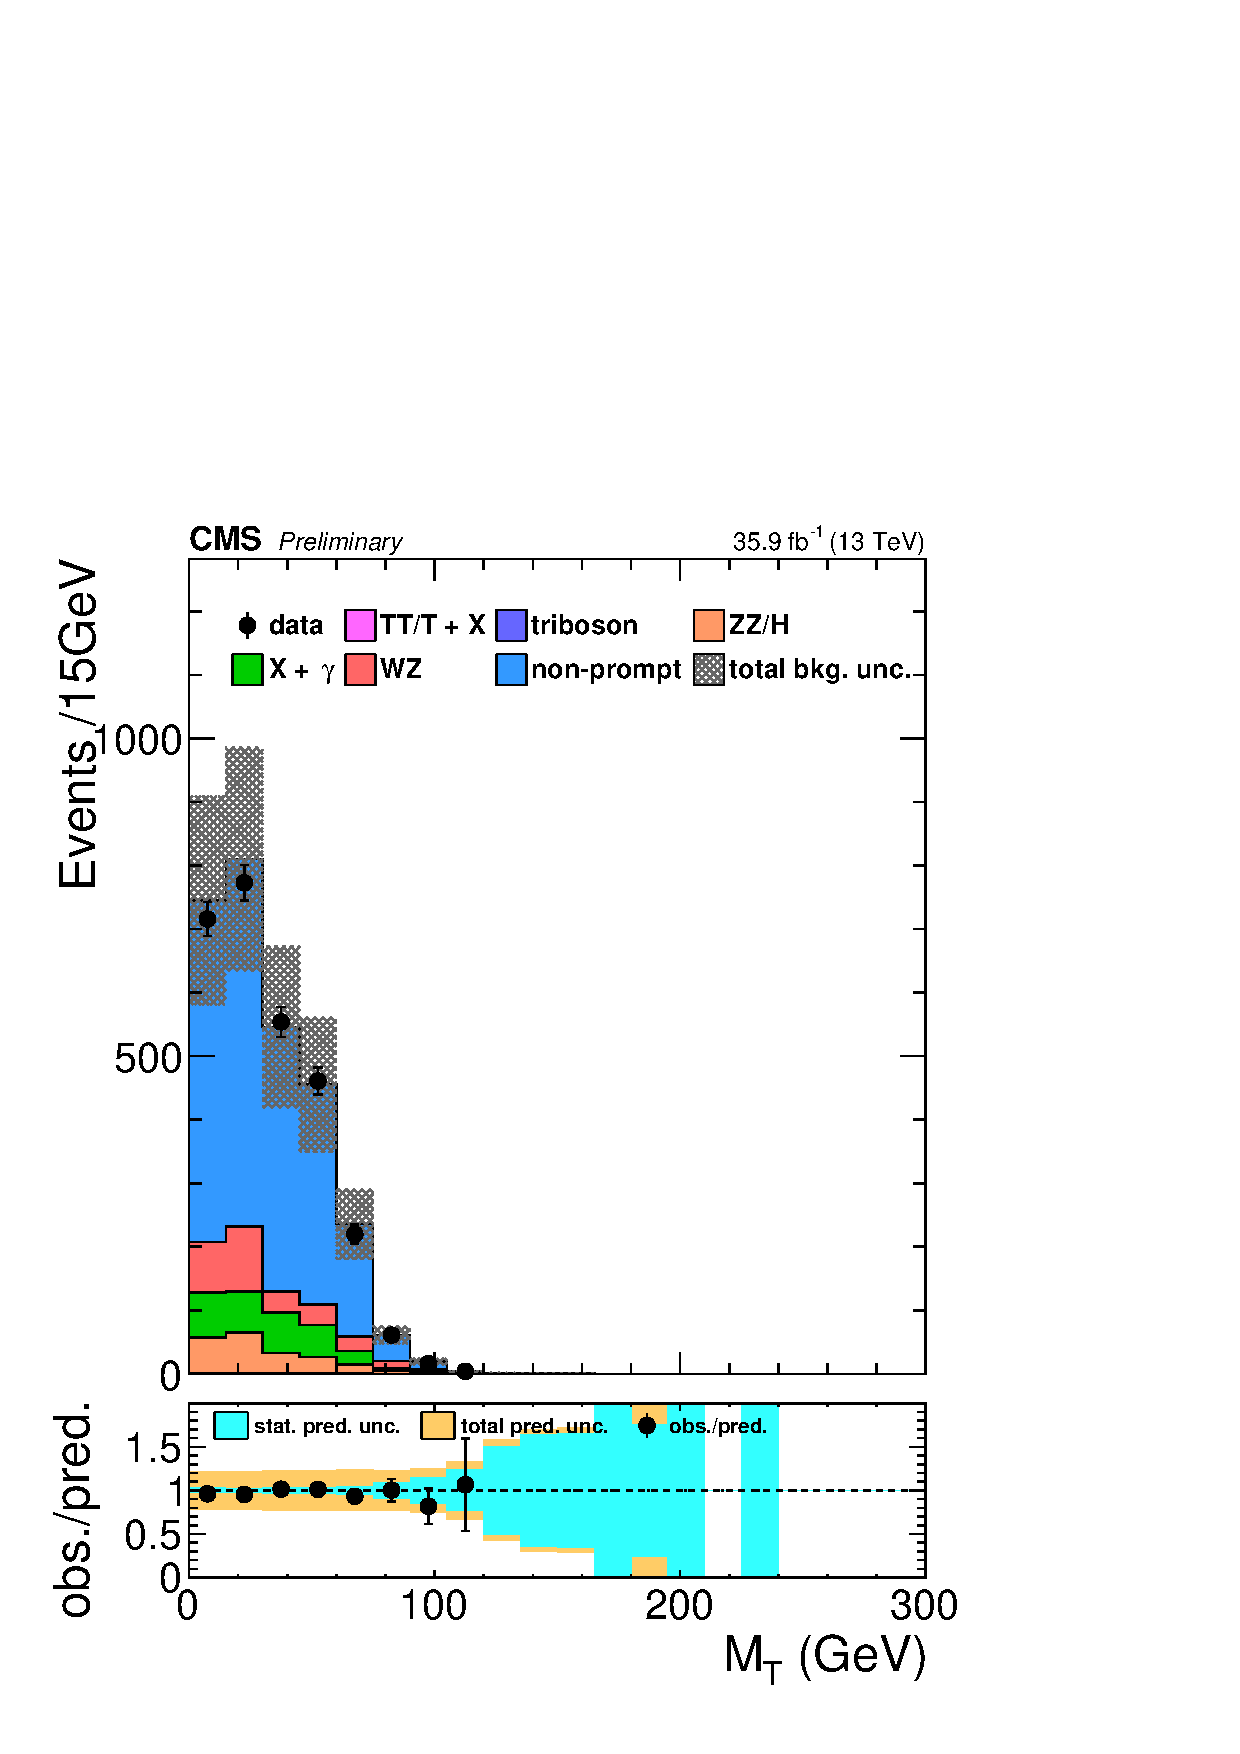
\includegraphics[width=.30\textwidth]{Figures/c5/DYCR/inclusive/mt_minMos_DY.pdf}\\
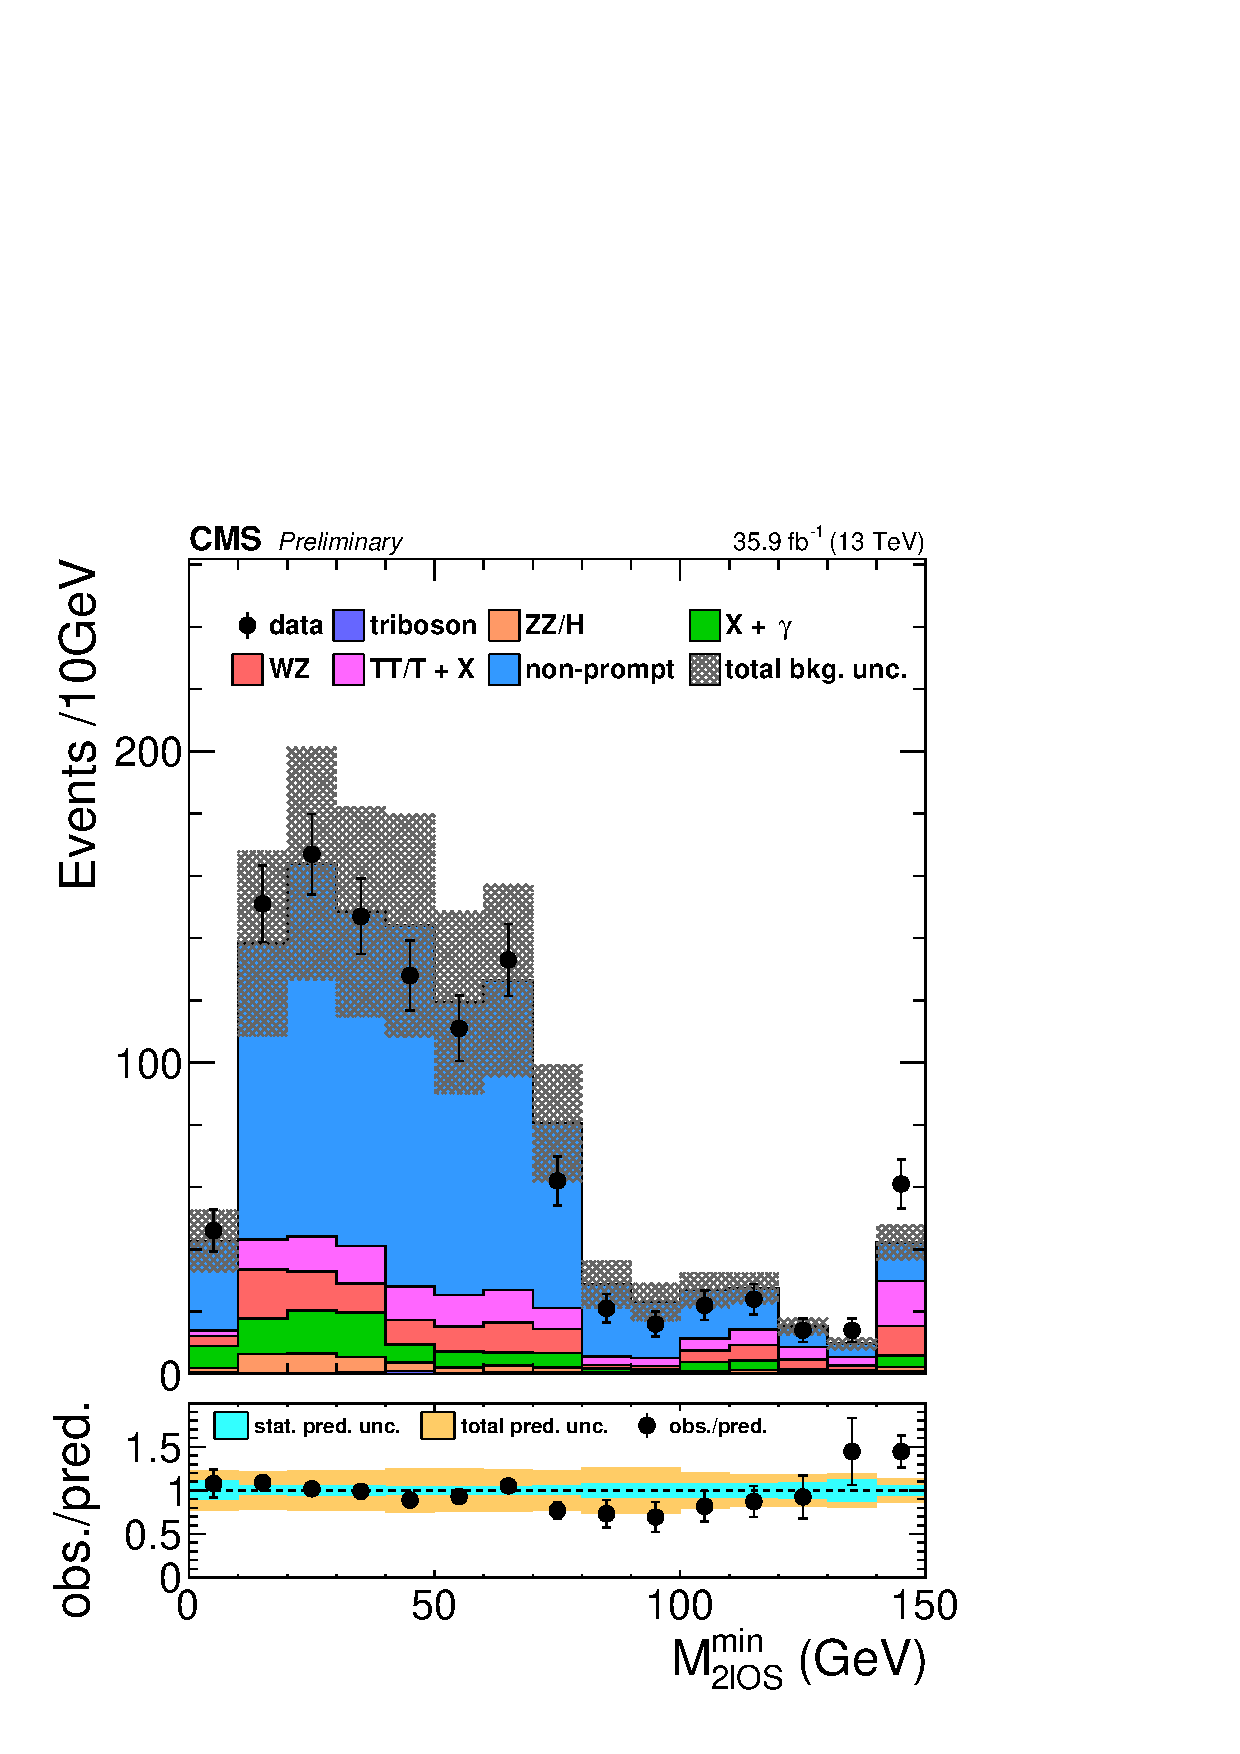
\includegraphics[width=.30\textwidth]{Figures/c5/TTCR/convVeto/minMos_TT.pdf}
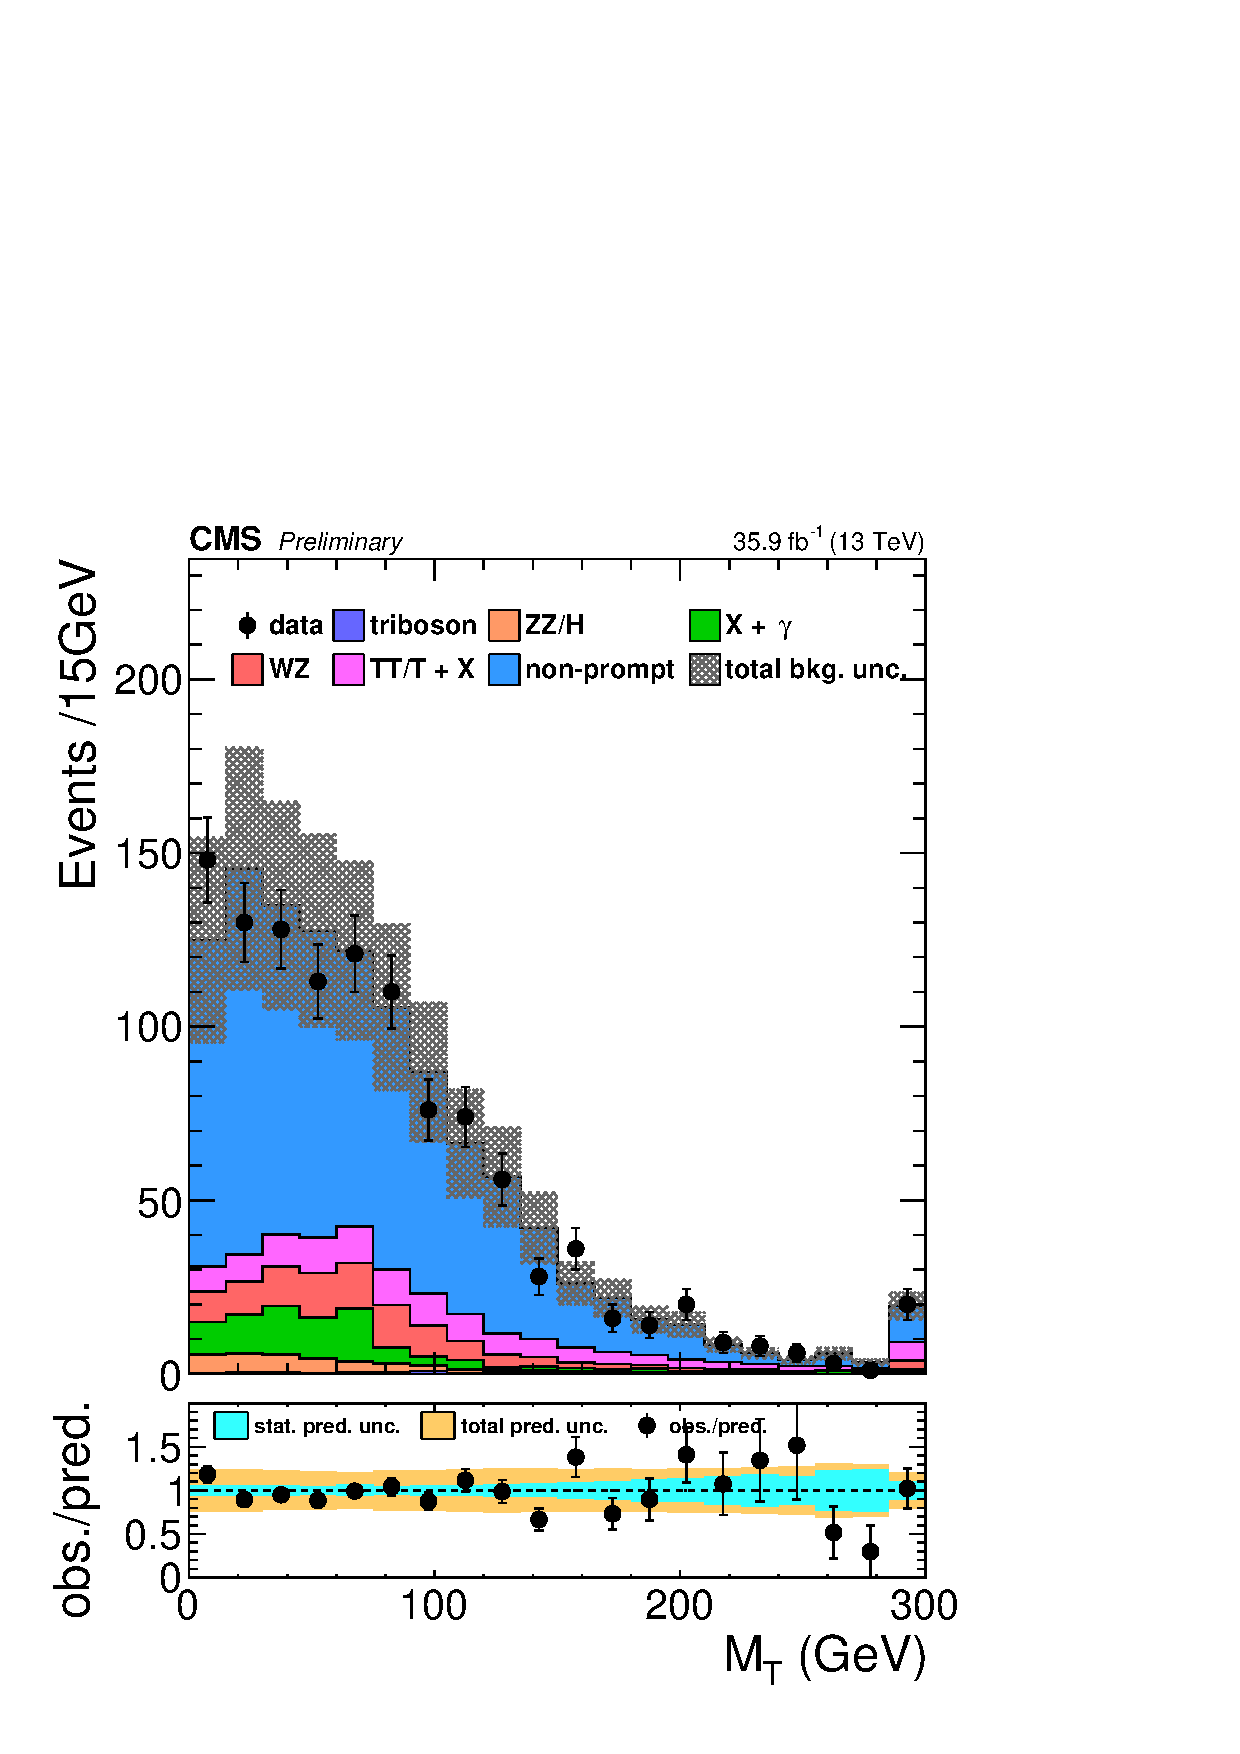
\includegraphics[width=.30\textwidth]{Figures/c5/TTCR/convVeto/mt_minMos_TT.pdf}
\caption{Comparison of data to background prediction in the Drell-Yan
  (top) and \ttbar (bottom) enriched control region,
  for \mmin and \mtmin. \willem} 
\label{fig:npvalidation}
\end{figure}

\paragraph{\texorpdfstring{\ttbar}{ttbar} enriched control region:}
The \fr for light-flavor and heavy-flavor jets is expected to be
different because of their different structure, and possibilities to
nonprompt leptons. In particular beauty quarks might decay
semi-leptonically, resulting in a harder leptons. As discussed earlier, the \fo working point used in this analysis is tuned in such a way that the \fr is expected to be nearly identical for light- and heavy-flavor jets. If this is the case, the \fr should also predict the background due to \ttbar  in a control region enriched in this process.
For this purpose we select events with at least one loosely b-tagged jet. 
For events with an OSSF pair, we exclude events within a 15\GeV window
around the Z-mass for both \mlll  and the best Z-candidate
mass. Additionally, these events are vetoed if they contain an OSSF
pair with mass below 12\GeV in order to suppress the contamination
from W$\gamma^{*}$ and conversions. Good closure is observed in Figure~\ref{fig:npvalidation}, further strengthening our confidence in the data-driven prediction of the nonprompt background.



Considering the results in both the \ttbar and Drell-Yan enriched control regions, we assign a flat 30\% uncertainty to this background prediction. 

\subsection{Background from prompt leptons}
As described in Section~\ref{sec:c4wz_zz}, sizable background
contributions come from ZZ production and from associated production of
\PW and \PZ bosons.

The predictions of those backgrounds with prompt leptons are obtained
from simulations. First, three specific control
regions enriched respectively with either 
ZZ or WZ or conversions processes are defined. Thus, the normalization weights are
extracted and the MC predictions are validated in
specific kinematic distributions. \\
To measured the normalization factors, a simultaneous fit of the three
control regions has been performed on the data yields and simulation yields. 
The ratios are then
applied to scale the predicted yields.  \\
In addition, it was checked the contamination of possible signal events in the
control regions and it was found negligible considering as \mixpar the
ones close to the sensitivity of the analysis. \\
The control regions and the results from the validations are
discussed in the following paragraphs.

\subsubsection{ZZ background validation and normalization}
Due to the fourth lepton veto, we can define a 4$\ell$ control region,
fully orthogonal to any of the search regions in which we can
normalize the ZZ cross section to data. We define a control region
with 4 \ti  leptons, with two OSSF pairs, both having a mass on-\PZ;
events with a loose b-tagged jet are vetoed. With the above requirements, this control region is extremely pure in ZZ, with other processes being almost negligible.
In the given control region, we measure the ZZ normalization by doing a maximum likelihood fit of the ZZ signal hypothesis, including the same treatment of systematic uncertainties as done for the interpretation of the HNL exclusion limits shown later in this text. This procedure yields the following scale factor:
$\text{data}_{\PZ\PZ}/\text{MC}_{\PZ\PZ} = 1.03_{-0.10}^{+0.11}$

Then, we check the prediction of the kinematic shapes in data and MC,
a few examples of which can be found in
Figure~\ref{fig:validation}. Overall data and MC predictions match well;
in the top-right plot in Figure~\ref{fig:validation} at low $m_T$ the
predictions from MC are within the experimental and theoretical
uncertainties, at large $m_T$ values there are still remaining
discrepancies. Thus we add 25\% systematic uncertainty for events with
$m_T> 75$\GeV, larger than the normalization uncertainty.

\subsubsection{WZ background normalization and validation}\label{sec:promptwz}
As described earlier, events in which the OSSF pair with the mass
closest to that of the Z boson fell within 15\GeV of the Z mass were
vetoed in order to suppress the WZ background. Because of this veto we
can employ this region to validate and normalize the WZ background. We
select 3 \ti  leptons and require \ptmiss> 50\GeV.
The sample used here has a large, known, overestimation of
the cross section, making it necessary to perform a cross section
measurement in our control region. This is done in the same way as for
the previously mentioned ZZ background, and the following scale factor
is obtained: $\text{data}_{\WZ}/\text{MC}_{\WZ}= 0.652_{-0.058}^{+0.061}$.

Figure \ref{fig:validation} shows the distribution of the three
important analysis variables. An extremely good match is seen in the
\mmin  and \mtmin  distributions, which are used to bin the high mass
search regions in which WZ is the dominant background.


\begin{figure}[h]
\noindent
\makebox[\textwidth]{
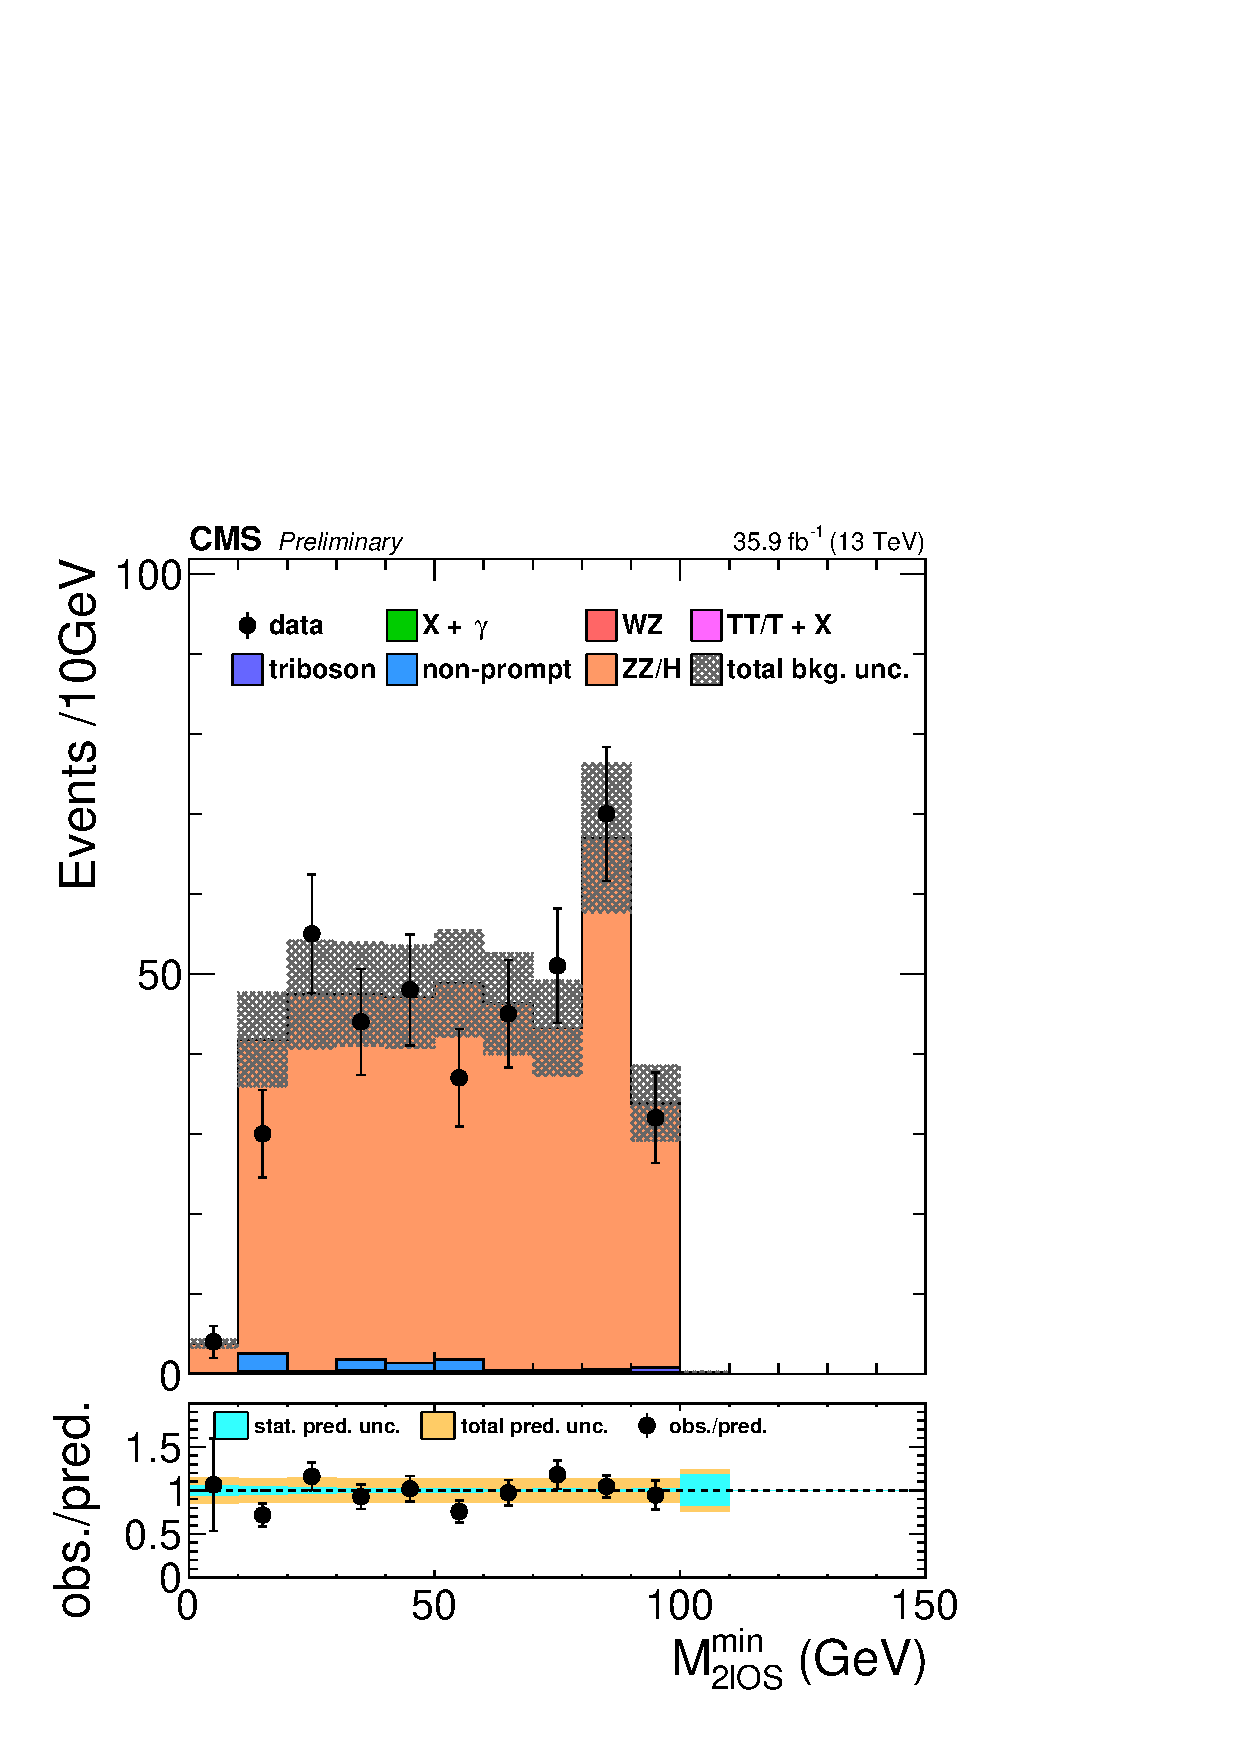
\includegraphics[width=.30\textwidth]{Figures/c5/ZZCR/ZZ/minMos_ZZ.pdf}
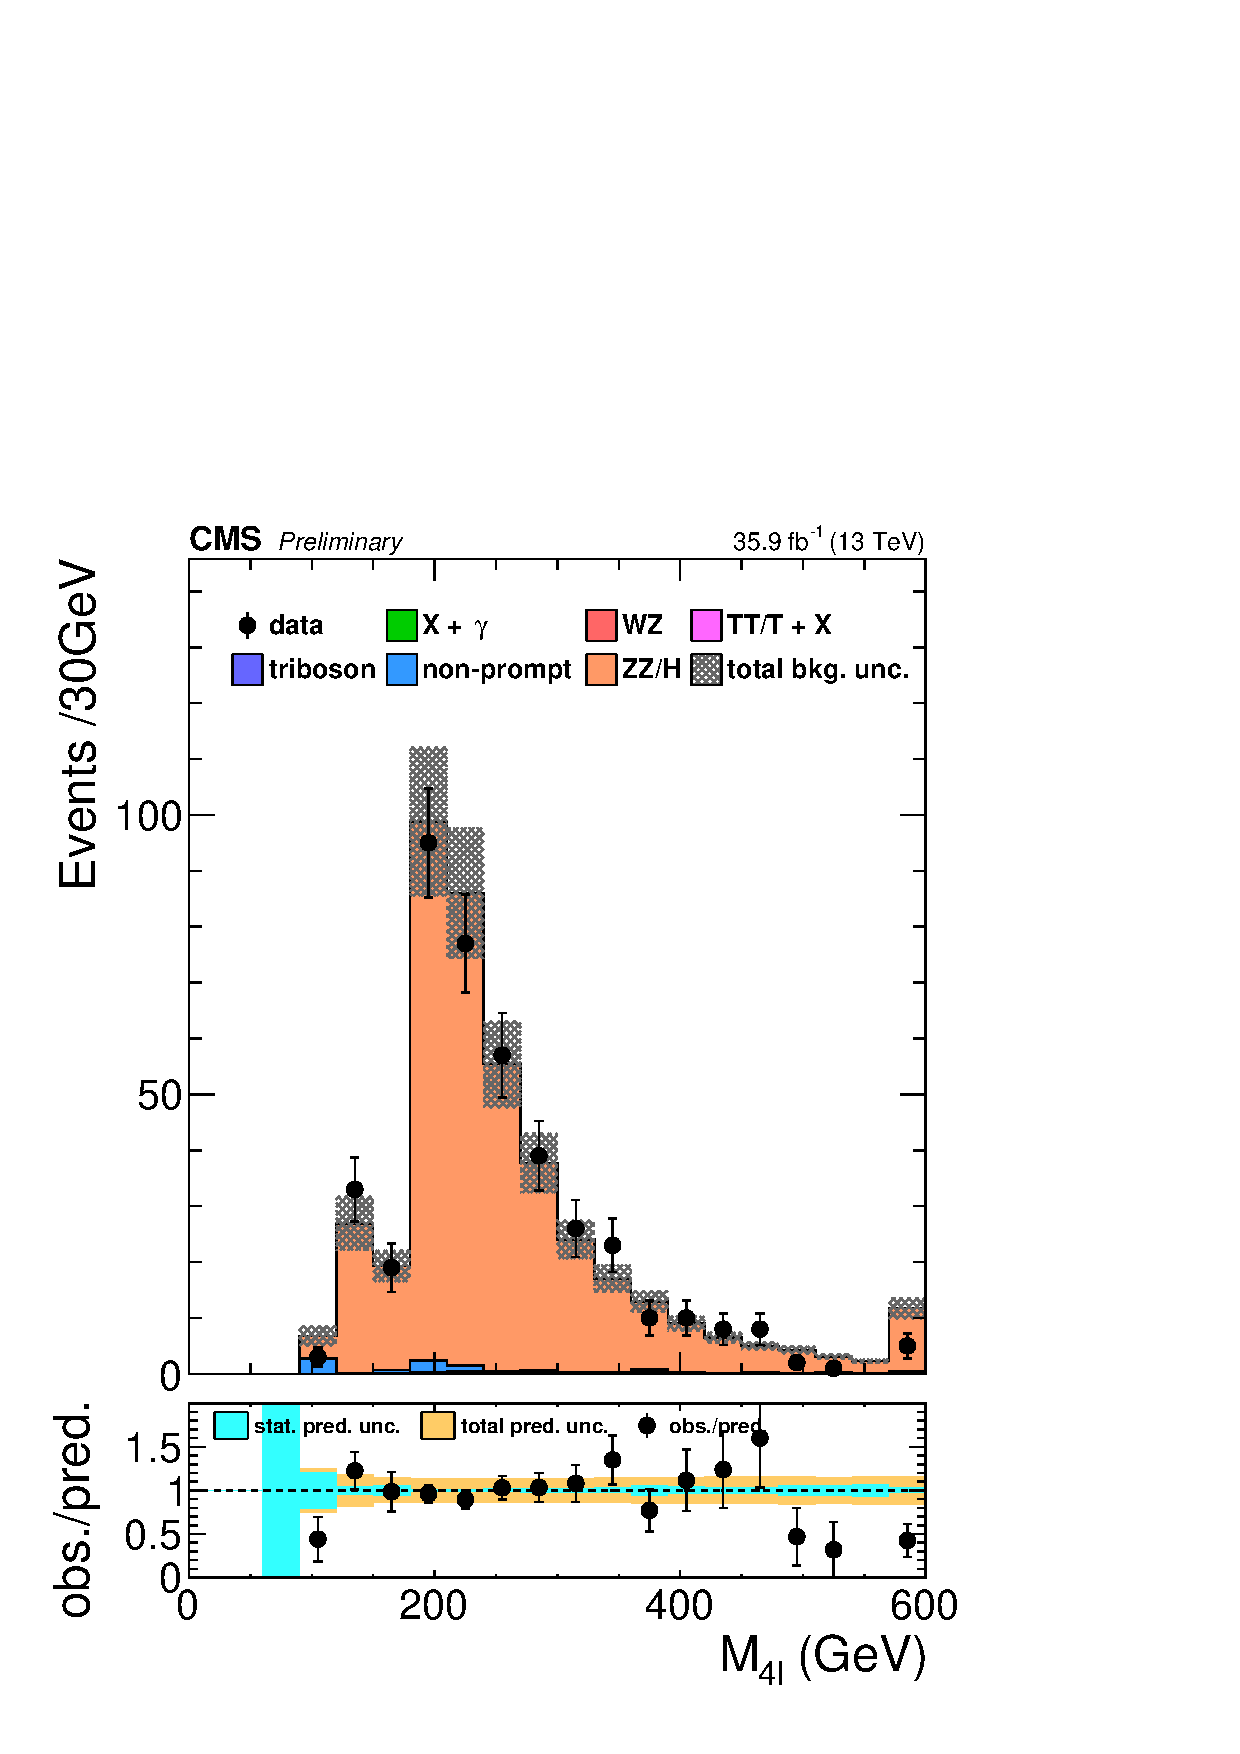
\includegraphics[width=.30\textwidth]{Figures/c5/ZZCR/ZZ/M4l_ZZ.pdf}
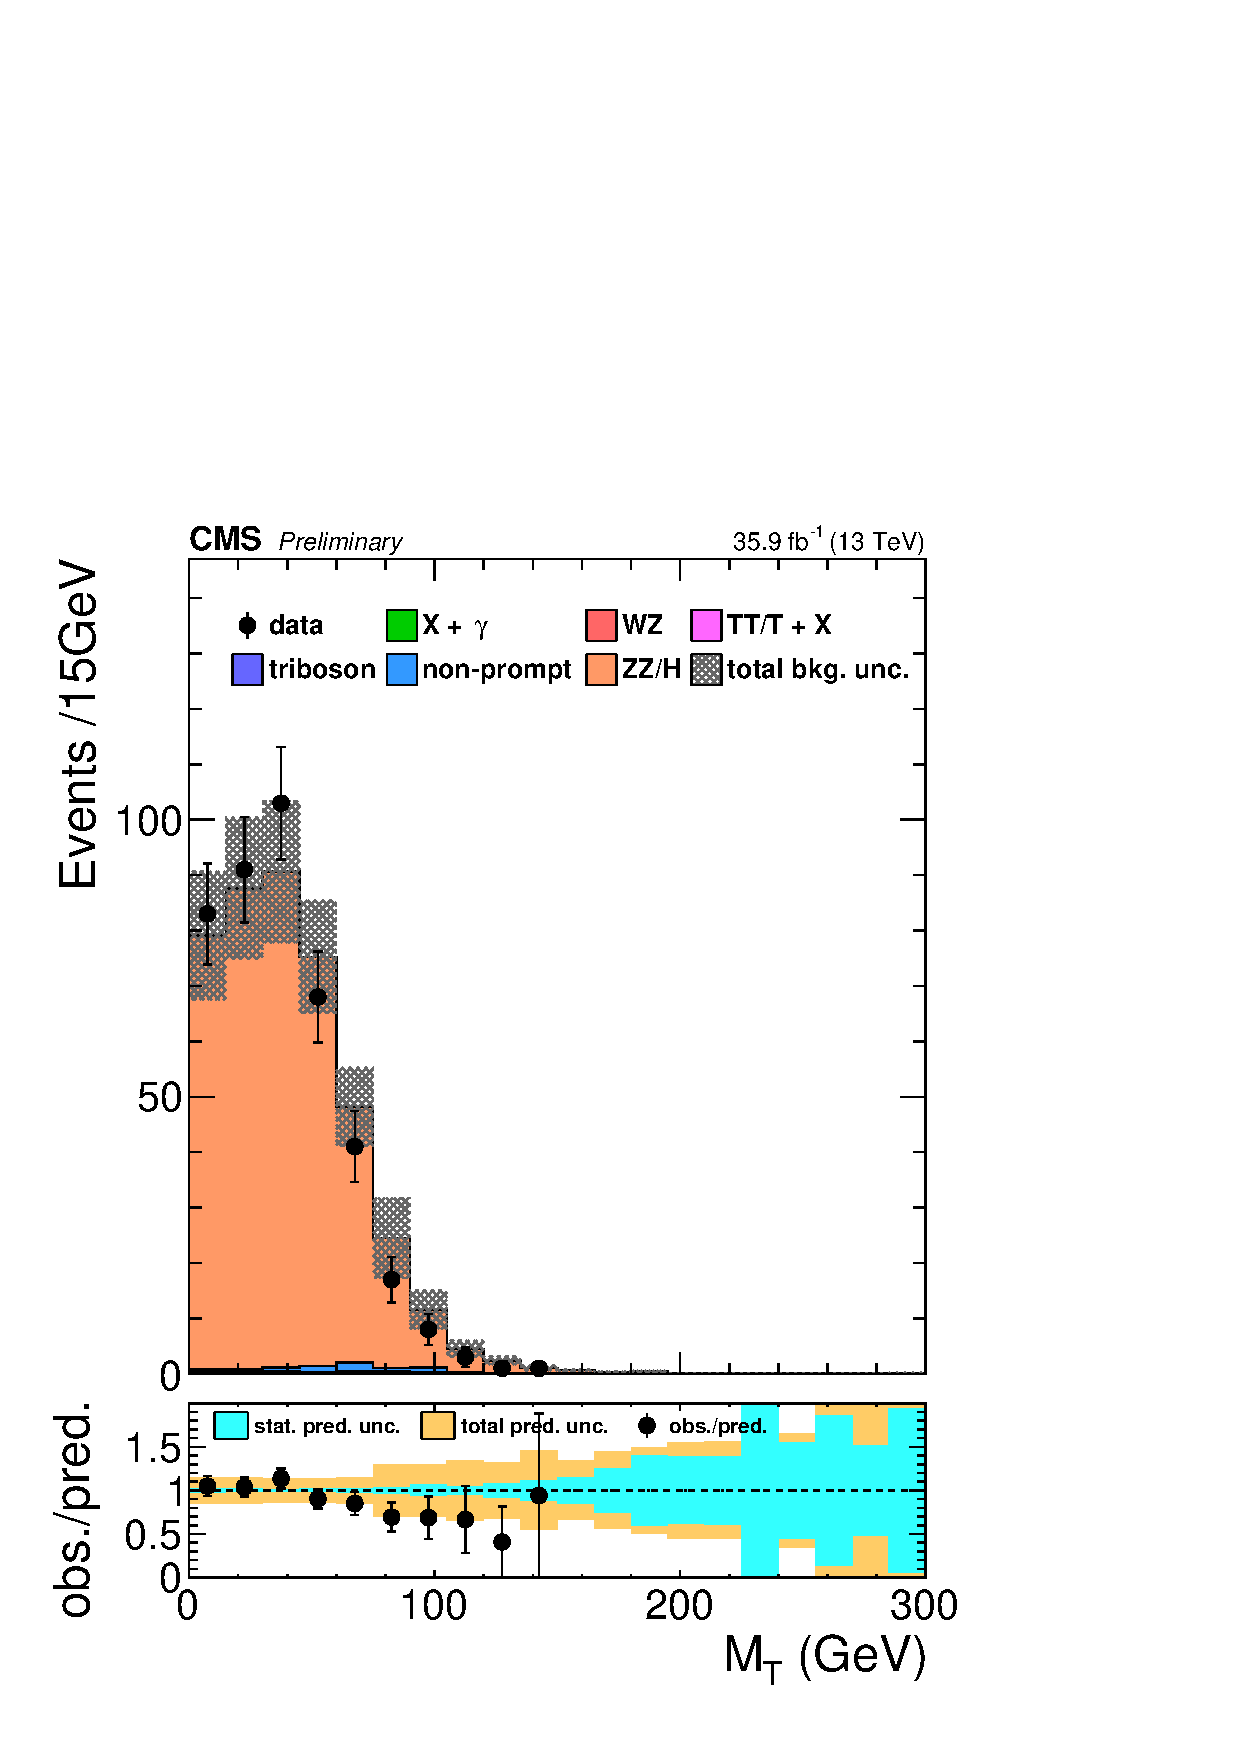
\includegraphics[width=.30\textwidth]{Figures/c5/ZZCR/ZZ/mt_minMos_ZZ.pdf}}\\
\makebox[\textwidth]{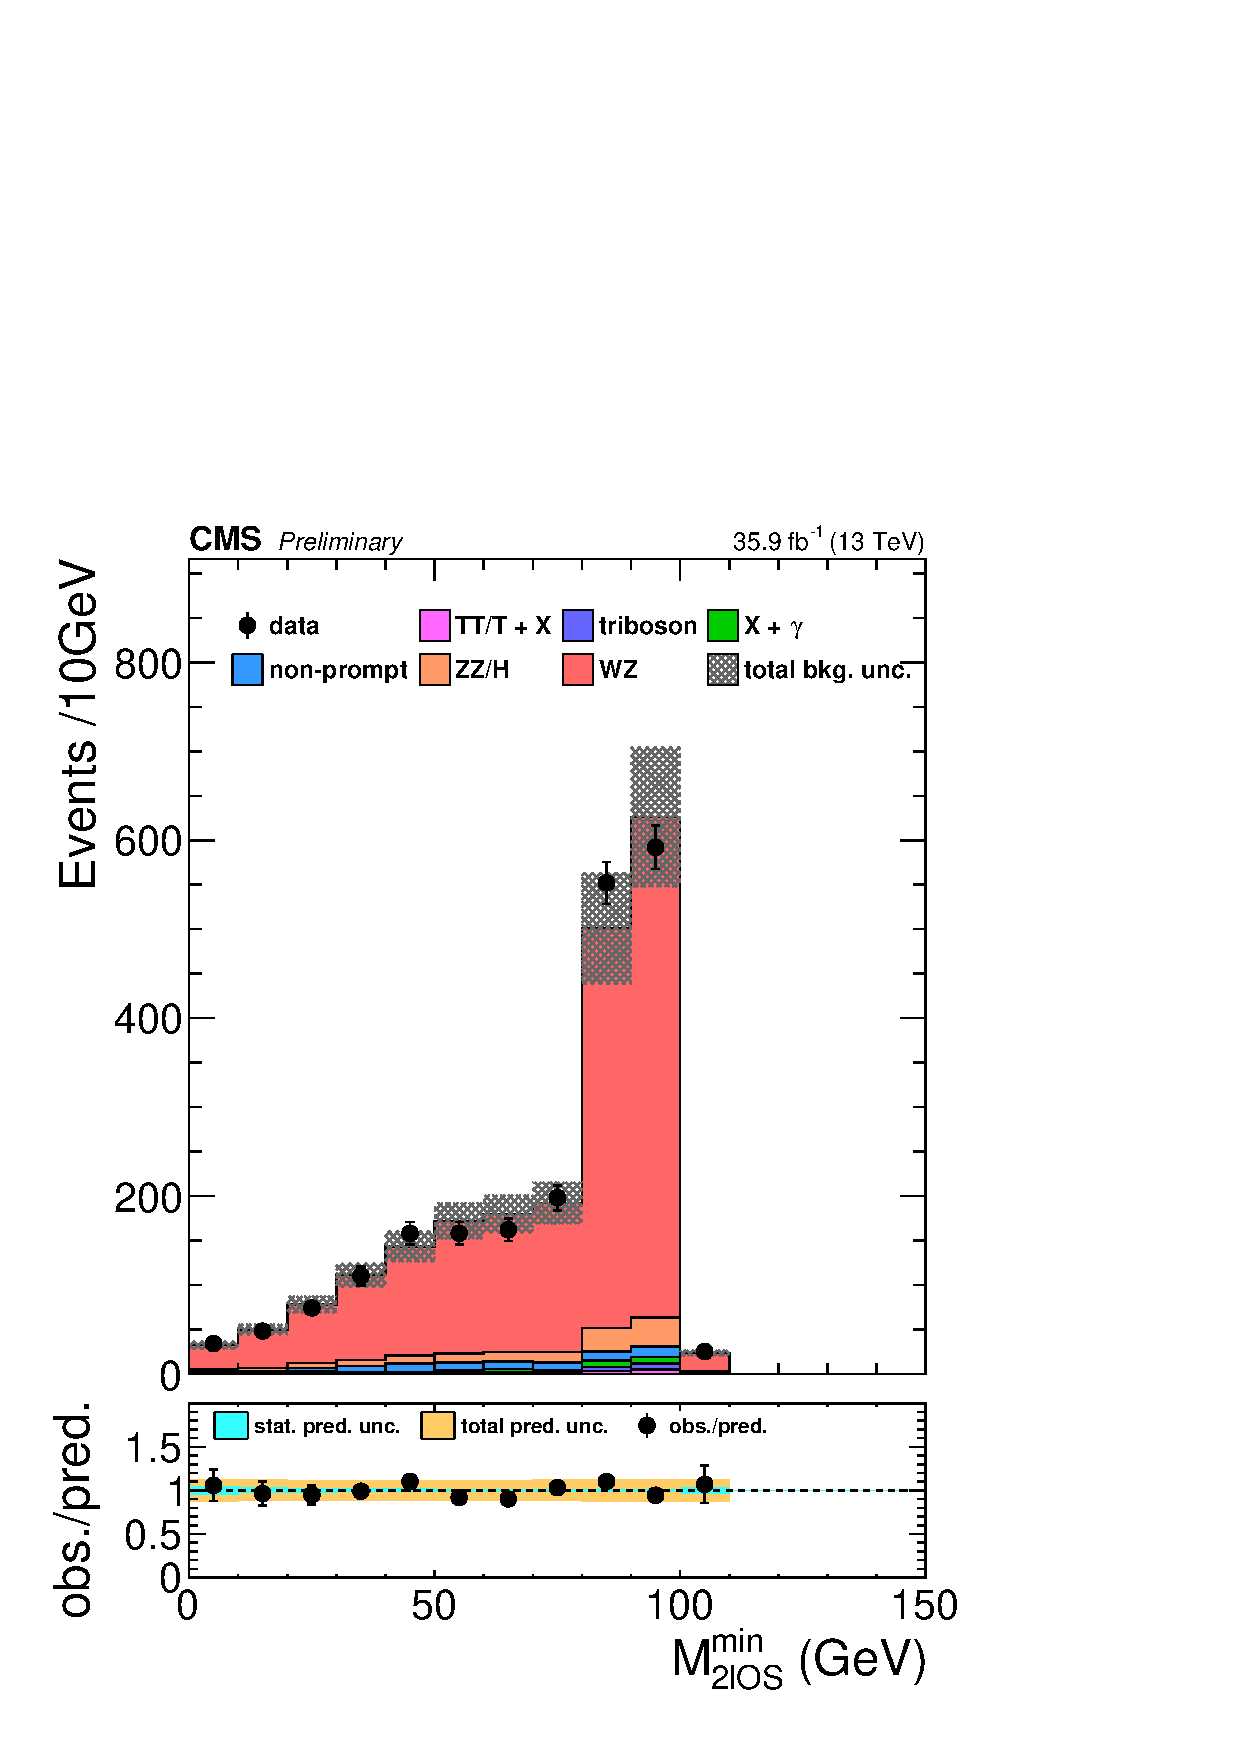
\includegraphics[width=.30\textwidth]{Figures/c5/WZCR/PtandMetCuts/minMos_WZ.pdf}
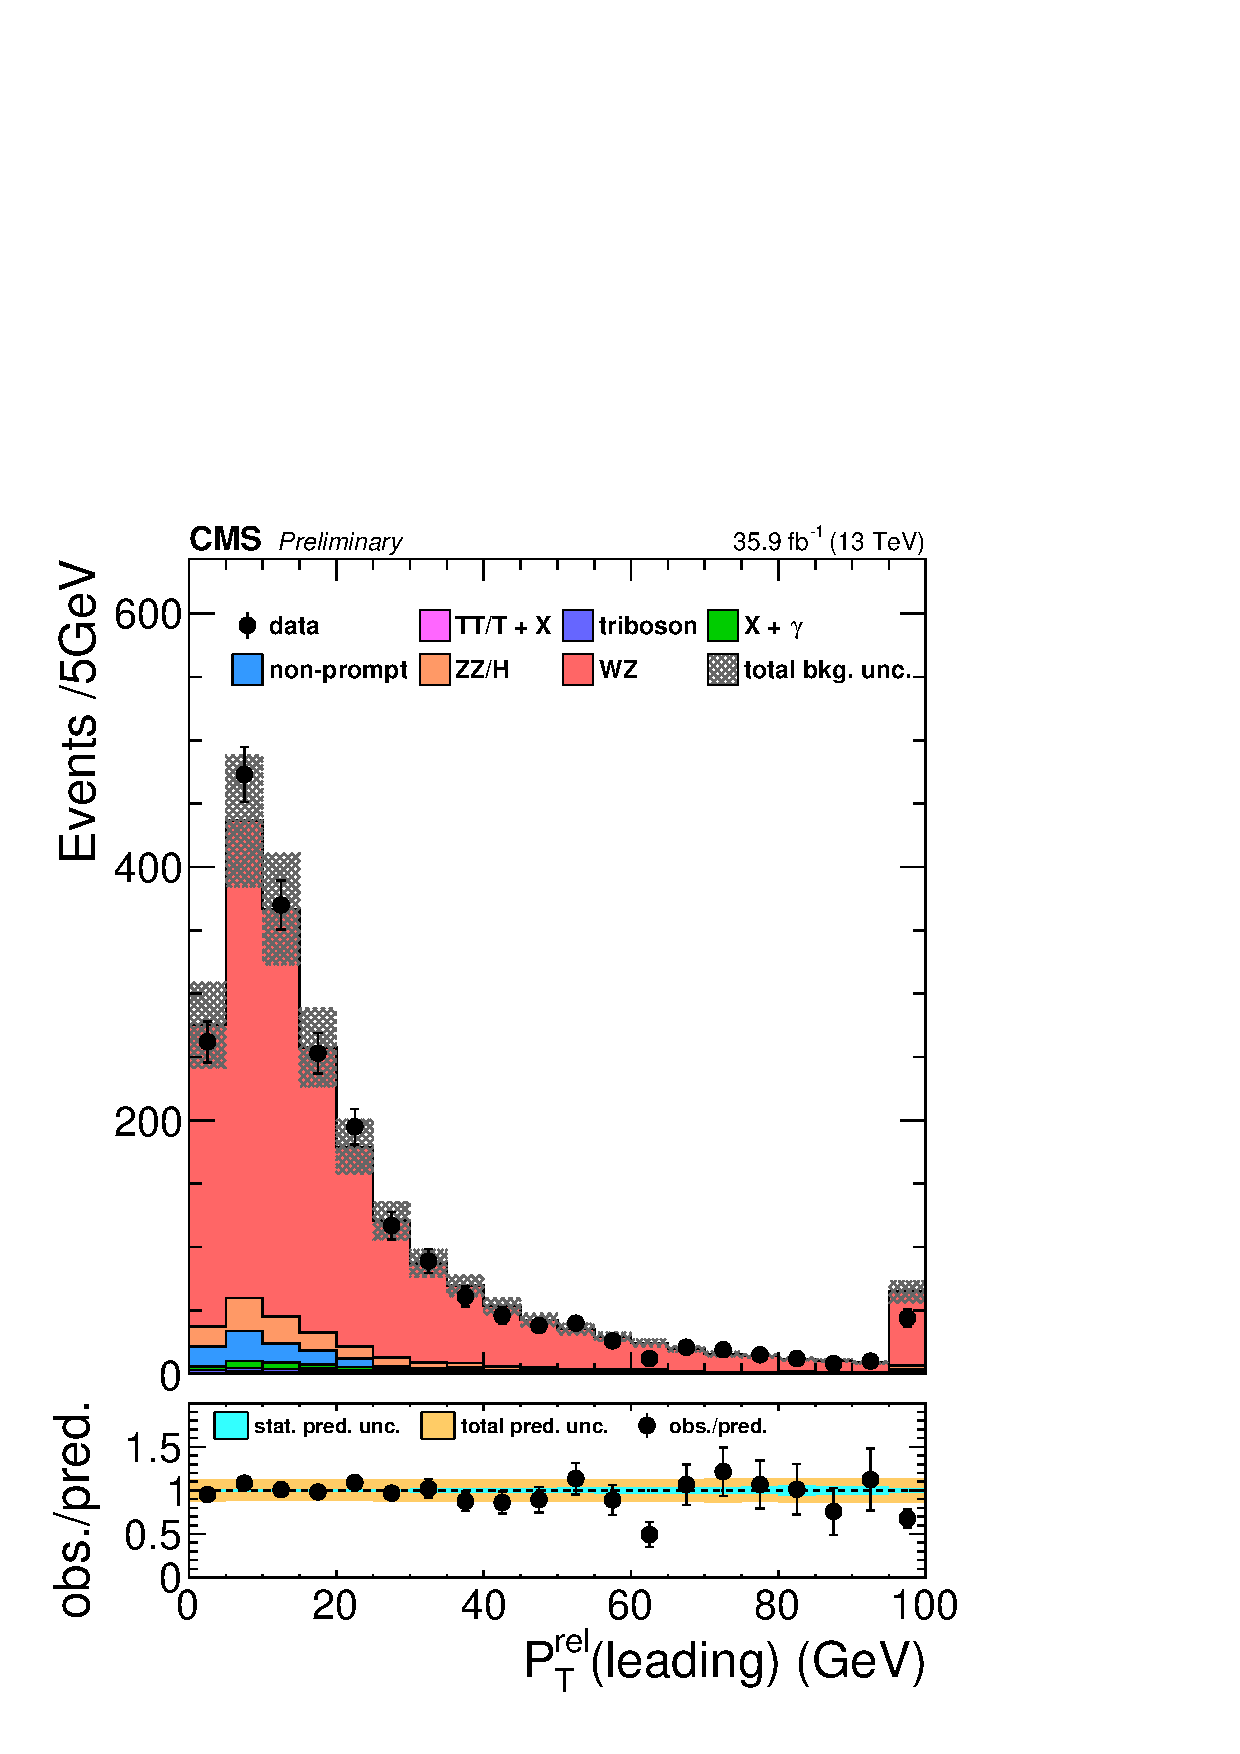
\includegraphics[width=.30\textwidth]{Figures/c5/WZCR/PtandMetCuts/Ptrel_le_WZ.pdf}
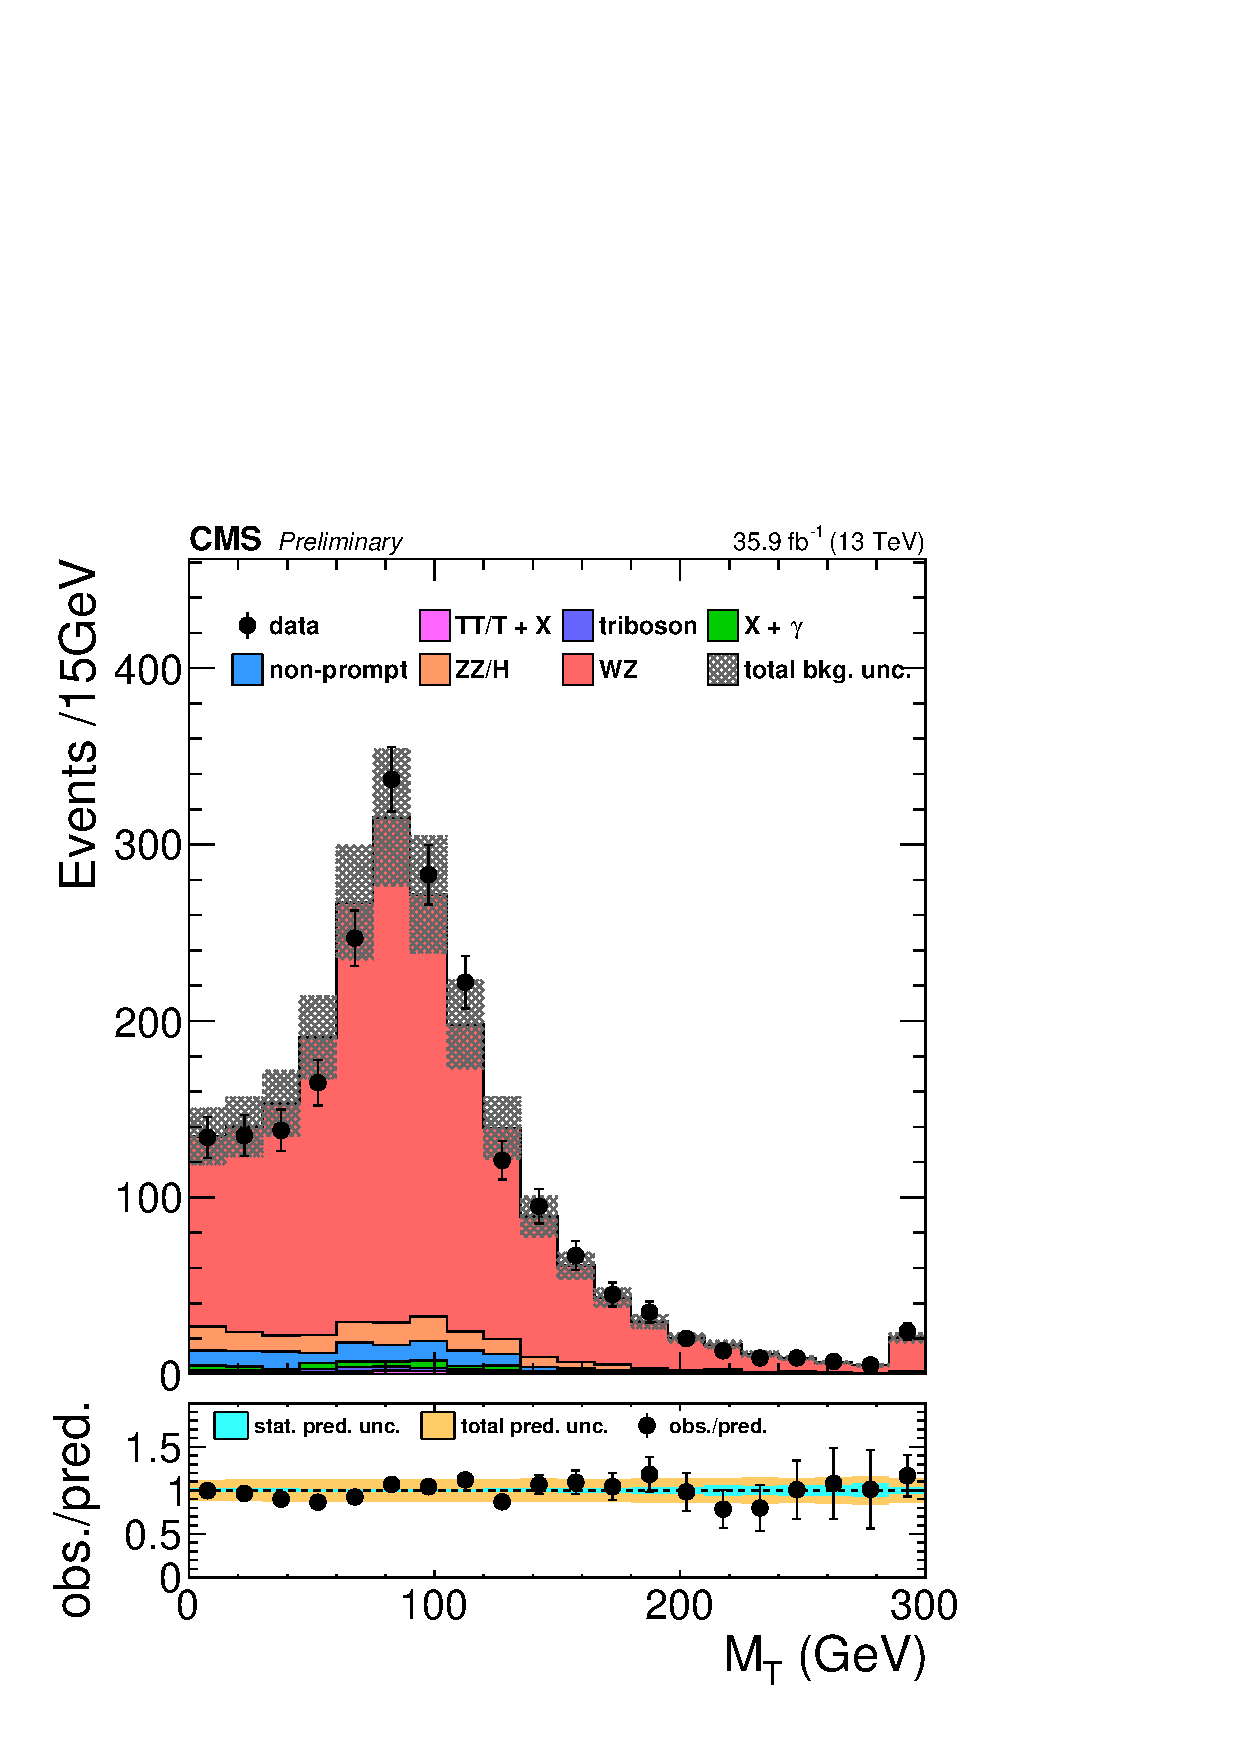
\includegraphics[width=.30\textwidth]{Figures/c5/WZCR/PtandMetCuts/mt_minMos_WZ.pdf}}
\caption{Comparison of data and MC in the ZZ control region (top) and in the WZ control region (bottom) for several kinematic variables, after normalization of the ZZ/WZ cross section. \willem} 
\label{fig:validation}
\end{figure}

\subsection{Background from internal and external $\gamma$ conversion}\label{sec:conversion}
Events in which a virtual photon decays (internal conversion) or in
which a  real photon converts into electron-positron pair by interacting with the
detector material (external conversion) constitute one of the main backgrounds in the
 low mass search bins, and in the low \mmin  and \mlll
  regions of the high mass search. The main contribution comes from
  asymmetric conversions. W$\gamma^{*}$ does not constitute a large contribution since the
 probability of both conversion decay products passing the analysis
 \pt requirements is rather small. Nonetheless it is important at very low
 masses, and vetoed in the low \mlll  part of the high mass search
 regions with OSSF pairs by removing events where an OSSF pair has mass below 5\GeV.

In order to normalize and validate this background we use a control
region defined requiring the presence of a OSSF pair and \mlll to be compatible with the Z mass within a 15\GeV
window. Additionally, the OSSF pair with the mass closest to that of Z
is required to have a mass below 75\GeV in order to remove the
contribution of Drell-Yan and WZ to this control region. The Z$\gamma$
cross section is normalized with respect to the data in this control
region. The obtained scale factor is:
$\text{data}_{\PZ\gamma}/\text{MC}_{\PZ\gamma} = 0.95_{-0.08}^{+0.08}$

The validation of the internal-external conversion background is shown
in Figure~\ref{fig:convvalidation}. It is observed a good agreement
between data and MC, but considering the small discrepancies at large
$p^{leading}_{T}$ we apply an additional 15\% systematic uncertainty to the modeling of conversions.

\begin{figure}[h]
\centering
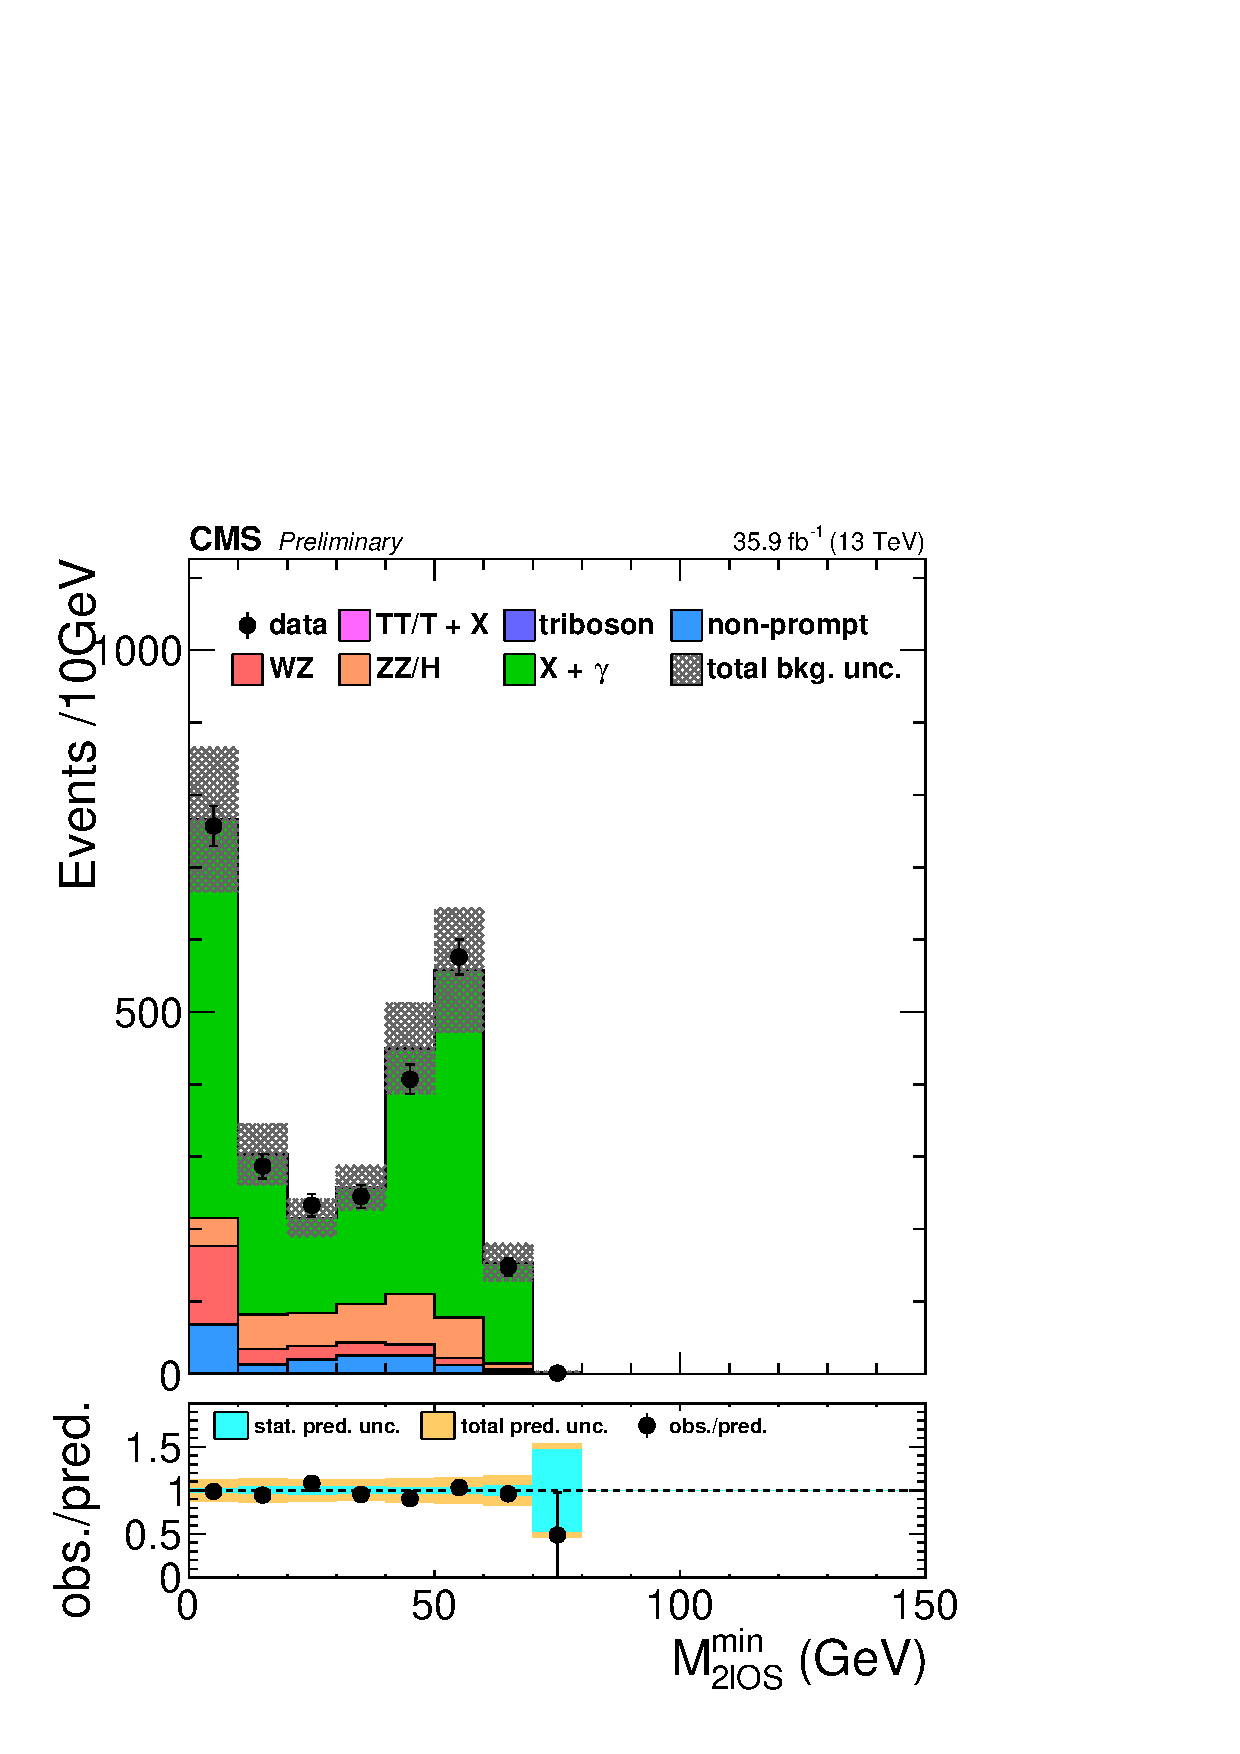
\includegraphics[width=.30\textwidth]{Figures/c5/convCR/combined/minMos_Xgamma.pdf}
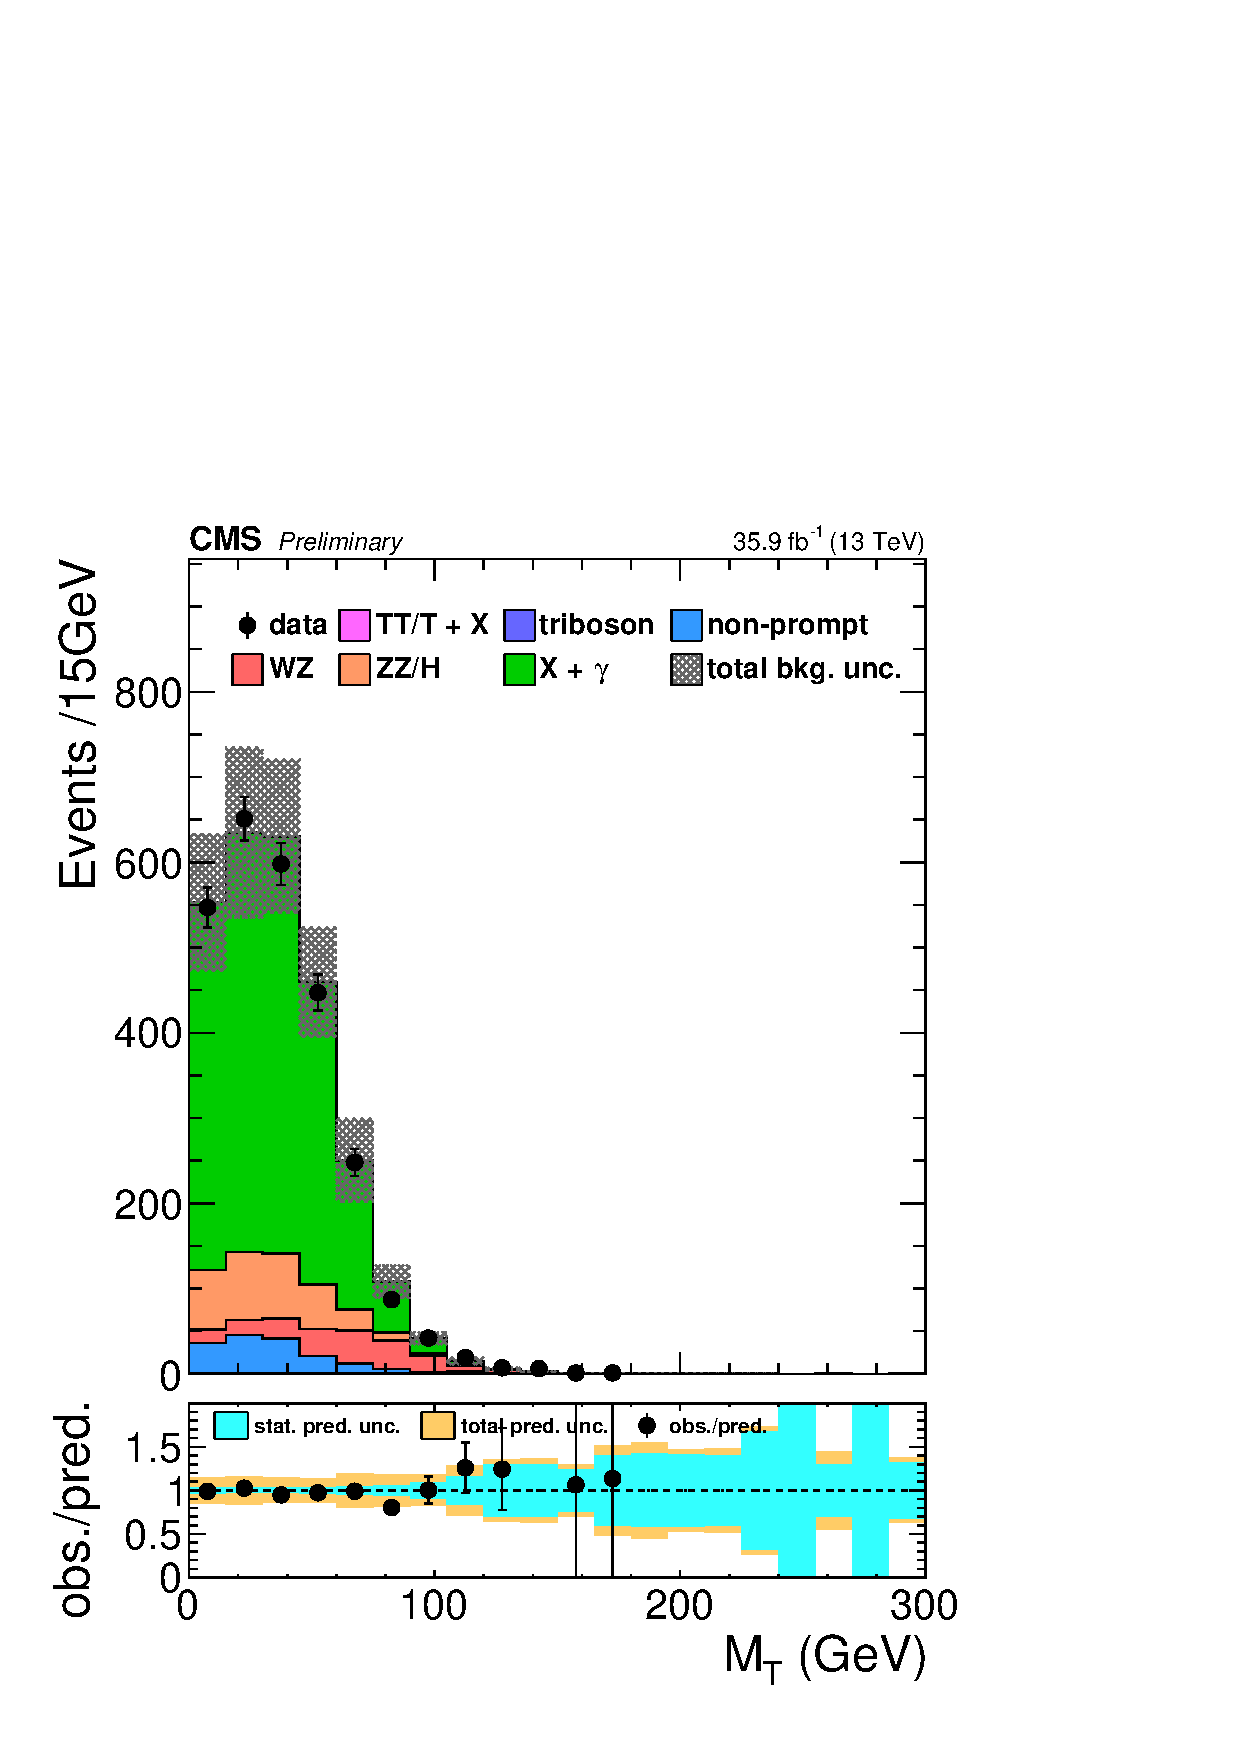
\includegraphics[width=.30\textwidth]{Figures/c5/convCR/combined/mt_minMos_Xgamma.pdf}
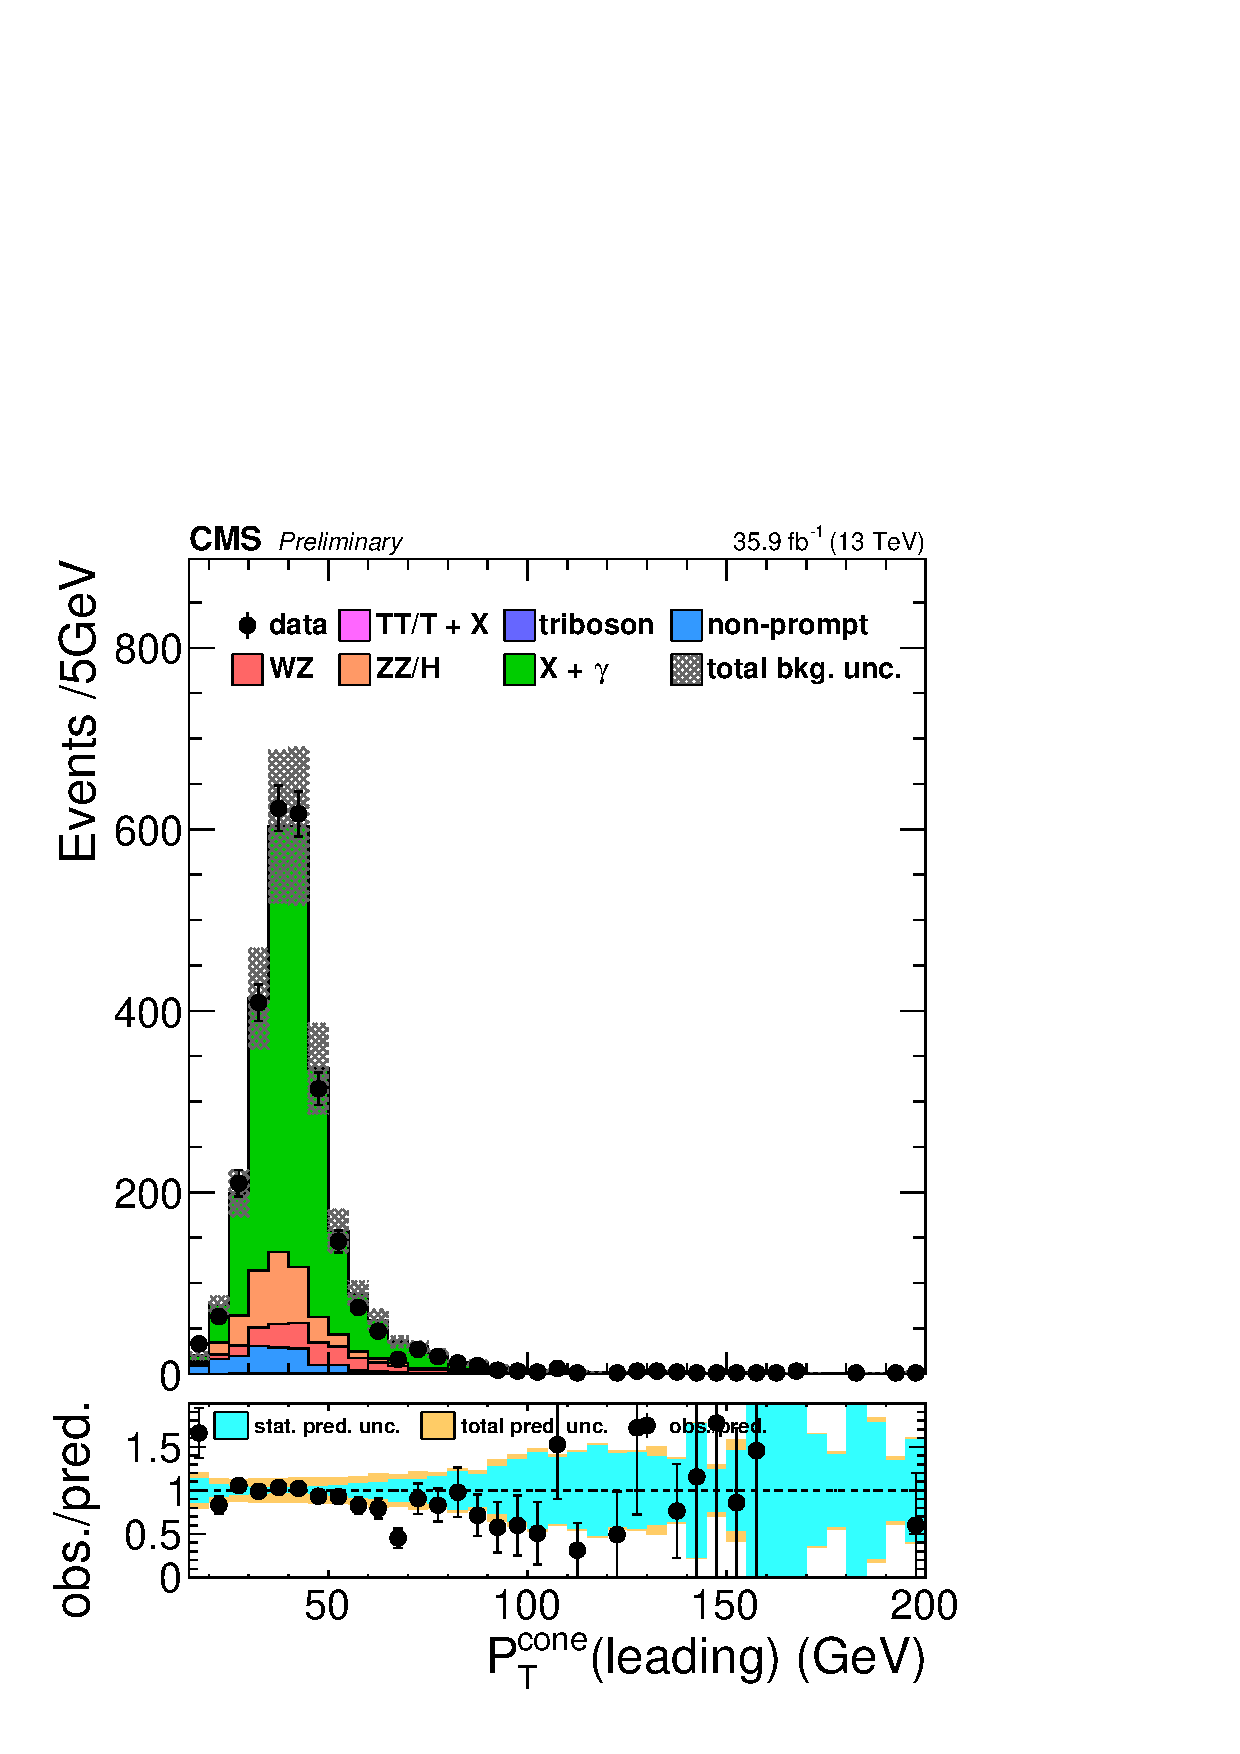
\includegraphics[width=.30\textwidth]{Figures/c5/convCR/combined/ConePt_le_Xgamma.pdf}\\
\caption{Comparison of data and MC in the conversion control region for the most important kinematic variables, after normalization of the Z$\gamma$ and W$\gamma$ cross sections. \willem} 
\label{fig:convvalidation}
\end{figure}

%%%%%%%%%%%%%%%%%%%%%%%%%%%%%%%%%%%%%%%%%%%%%%%%%%%%%%%%%%%%%%%%%%%%%%%%%%%%%%%%%%%%%%%%%%%%%%%%%%%%%%%
%%%%%%%%%%%%%%%%%%%%%%%%%%%%%%%%%%%%%%%%%%%%%%%%%%%%%%%%%%%%%%%%%%%%%%%%%%%%%%%%%%%%%%%%%%%%%%%%%%%%%%%
%%%%%%%%%%%%%%%%%%%%%%%%%%%%%%%%%%%%%%%%%%%%%%%%%%%%%%%%%%%%%%%%%%%%%%%%%%%%%%%%%%%%%%%%%%%%%%%%%%%%%%%
\clearpage
\section{Systematic uncertainties}
The analysis is prone to several sources of systematic uncertainties which are listed below in table~\ref{tab:syst}. 

The jet energy scale uncertainty varies between 0 and 3\%, depending on the search region. 
This uncertainty affects other event quantities such as the b tag veto, $\ptmiss$, and $\mtmin$, 
and is computed by shifting the energies of all jets coherently and propagating the variation to all these kinematic variables~\cite{jecDataMC}. 
Correlation effects due to the migration of events from one search region to another are taken into account. 
Similarly, the b jet veto efficiency is corrected for the differences between data and simulation, 
and an associated uncertainty in this correction is derived to be~1--5\%~\cite{btagSF}. 
The uncertainty in the modeling of pileup is computed by modifying the minimum bias cross section by 5\%~\cite{PUtwiki},
and it is measured to be 1--5\%, depending on the search region. 
The uncertainty in the integrated luminosity is 2.5\%~\cite{CMS-PAS-LUM-17-001}.

All sources of systematics that are labeled as "shape" are computed by varying the yields across the search regions 
bin-by-bin using the recommended procedures to assess the listed sources of systematic uncertainty.  

The dominant uncertainty in the total background prediction is the statistical uncertainty in the nonprompt leptons background estimation,
which comes from the limited number of events in the application region. The systematic uncertainty on the nonprompt prediction has
a subleading value. 

In the high-mass search regions with the OSSF pair present the dominant background is from WZ and external/internal conversion process, hence
the uncertainties on this process as well as MC-modeling uncertainties become more important.

\begin{table}[h]
    \caption{Summary of systematic uncertainties in the event yields in the search regions and their treatment. 
   Uncertainties are allowed to vary only the normalization of all the bins at once, or both the shape and the normalization 
   (allowing for different correlations across the bins).  
The upper group lists uncertainties related to experimental effects for all processes whose yield is estimated from simulation;
the middle group lists uncertainties in these yields related to the event simulation process itself.
The third group lists uncertainties for background processes whose yield or normalization is estimated from data.}
\label{tab:syst}
\centering
\resizebox{0.9\textwidth}{!}{
\begin{tabular}{lcc}
\hline
Source          & typical uncertainty value (\%) & Treatment \\
\hline
e/$\mu$ selection &  3 (per $\ell$) & normalization \\
Trigger efficiency &  2--5 & normalization \\
Jet energy scale & 0--3 & shape \\
b tag veto & 1--5 & shape \\
Pileup & 1--5 & shape\\
Integrated luminosity & 2.5 & normalization \\
\hline
Scale variations & 1-15 & shape \& normalization \\
PDF variations & 0.1-1 & shape \\
Other backgrounds & 50 & normalization \\
MC samples statistical precision & 1--30 & normalization \\
\hline
Nonprompt leptons  & 30 & normalization \\
Nonprompt leptons ($\PW$, $\PZ$ bkg. subtraction) & 5--20 & shape \\
$X\gamma$ normalization & 15 & normalization \\
$\WZ$ normalization & 8.5 & normalization\\
$\PZ\PZ$ normalization & 25 & normalization\\\hline
\end{tabular}  }
\end{table}



\section{Results}\label{sec:result}

In the left part of Figure~\ref{fig:allSRplotMuon}(top) 
the expected and observed yields in each of the \emph{low mass search}
regions are shown, compared to the predicted yields of several HNL masses, with \mixpar = $10^{-5}$. These yields, together with their
statistical and systematic uncertainties can also be found in
Table~\ref{tab:YieldsLowmass}.  \\
The expected and observed yields in the \emph{high mass search regions},
compared to several HNL mass scenarios at \mixpar = $10^{-2}$, for
events with and without an OSSF pair are shown in
Figure~\ref{fig:allSRplotMuon}. All search region yields, with their
separate statistical and systematic uncertainties are listed in
Tables~\ref{tab:YieldshighmassOSSF} and
\ref{tab:YieldshighmassnoOSSF}. \\
We see no evidence of an excess in data beyond the SM background.
\small{
\begin{table}[h]
\centering
\caption{Observed (expected) event yields in the low-mass search region. The uncertainties
contain both the statistical and systematic components.}
\label{tab:YieldsLowmass}
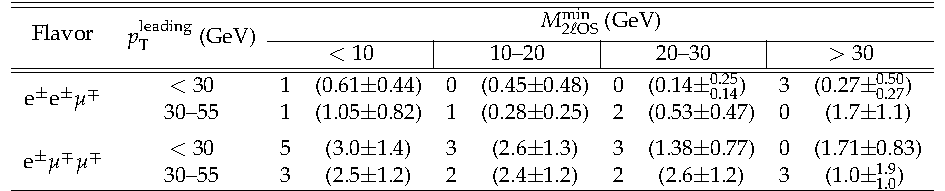
\includegraphics[width=0.65\linewidth]{Figures/c5/tables/CMS-EXO-17-012_Table_0A1.pdf}
\end{table}
\begin{table}[h]
\centering
\caption{Observed (expected) event yields in the high-mass search region for events with no
OSSF lepton pair. The uncertainties contain both the statistical and systematic components.}
\label{tab:YieldshighmassOSSF}
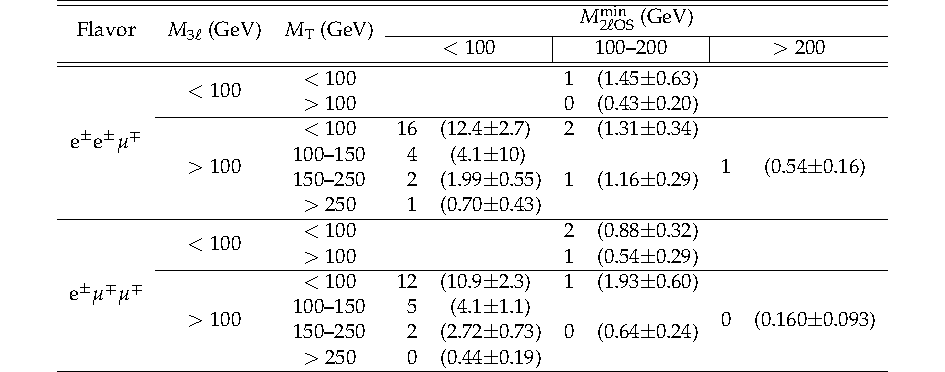
\includegraphics[width=0.7\linewidth]{Figures/c5/tables/CMS-EXO-17-012_Table_0A2.pdf}
\end{table}
\begin{table}[h]
\centering
\caption{Observed (expected) event yields in the high-mass search region for events with an
OSSF lepton pair. The uncertainties contain both the statistical and systematic components.}
\label{tab:YieldshighmassnoOSSF}
\includegraphics[width=0.7\linewidth]{Figures/c5/tables/CMS-EXO-17-012_Table_0A3.pdf}
\end{table}
}
\begin{figure}[h]
\noindent
\makebox[\textwidth]{\includegraphics[width=1\textwidth]{Figures/c5/expectedYields/CMS-EXO-17-012_Figure_001.pdf}}
\caption{Observed and expected event yields as a function of \mmin and
  \mtmin for events with
at least two electrons (upper), and with at least two muons (lower). The contribution of each
background source is shown. The first 8 bins of each figure correspond to the low-mass region,
while the rest display the high-mass region. \willem}
\label{fig:allSRplotMuon}
\end{figure}

\clearpage
\subsection{Interpretation}
 The expected signal exclusion limits are calculated for
 several mass points using a simultaneous fit to every search region
 bin, together with the observed limit. This fit is done in the
 Asymptotic approximation. The upper limit set on the signal strength
 for each mass point can then be interpreted as a
 limit on the effective couplings of the HNL to SM neutrinos, \mixpare
 and \mixparm. Limits were explicitly calculated for HNL masses of 1, 2, 5, 10, 20, 30, 40, 50, 60, 80, 100,
 130, 150, 200, 400, 600, 800 and 1000\GeV. Using linear
 interpolation between the mass points and assuming only a coupling to either $\nu_{\mu}$ or $\nu_{\Pe}$,
 we obtain the exclusion limits shown in Figure~\ref{fig:limits}. It can be seen that the expected and
 observed limits agree well, within less than one standard deviation
 for almost every point, indicating that no significant excess beyond
 the SM expectations has been observed. 
\begin{figure}[h]
\centering
\includegraphics[width=.80\textwidth]{Figures/c5/limits/CMS-EXO-17-012_Figure_002-a.pdf}\\
\includegraphics[width=.80\textwidth]{Figures/c5/limits/CMS-EXO-17-012_Figure_002-b.pdf}
\caption{Exclusion region at 95$\%$ CL in the \mixpare vs. $m_N$ (top) and \mixparm vs. $m_N$ (bottom) planes.
The dashed black curve is the expected upper limit, with one and two standard-deviation
bands shown in dark green and light yellow, respectively. The solid black curve is the observed
upper limit, while the dotted black curve is the observed limit in the approximation of
prompt N decays. Also shown are the best upper limits at 95$\%$ CL from other collider searches
in L3~\cite{ACHARD200167}, DELPHI~\cite{Abreu:1996pa}, ATLAS~\cite{Aad_2015}, and CMS~\cite{Sirunyan:2018xiv}. \willem}
\label{fig:limits}
\end{figure}

\clearpage
\section{Summary}
In this chapter, the search for heavy neutral leptons in events with
three prompt
charged leptons is presented. The analysis
results were published in Physical Review Letters in early 2018~\cite{Sirunyan:2018mtv}.

The signature consists of three prompt charged leptons in any flavor combination of electrons
and muons.
No statistically significant excess of signal events over the expected
SM background was observed. At 95\% confidence level, upper limits were set on the mixing
parameters \mixpare and \mixparm. 
The excluded values are in the
range between $1.2\times 10^{-5}$ and $1.8$ for masses 
between 1\GeV and 1.2\TeV. 

The results were positively received by the community and highly appreciated
for the big effort that was put into extending the mass range and
improving the existing sensitivity at the time of the publication.
These were the first direct limits for HNL masses above 500\GeV and the first
limits obtained at hadron colliders for HNL masses below 40\GeV.
At large HNL masses, the results improved those previously published
by the ATLAS~\cite{Aad_2015} and CMS~\cite{Khachatryan_2015,Sirunyan:2018xiv}
experiments. In particular with respect to the ATLAS search the mass
range was substantially extended towards values below the \PW boson
mass. The previous CMS searches were carried out with the data
collected in 2012 at $\sqrt{s} = 8$\TeV, which corresponds to an
integrated luminosity of 19.7\fbinv. 
For the first time at hadron colliders, this search focuses on low HNL mass ranges
($ m_\hnl < $ 40\GeV) increasing the sensitivity reached by the
L3~\cite{ACHARD200167} and DELPHI~\cite{Abreu:1996pa} Collaborations
in the prompt case scenario.\\

The specification for the promptly decaying HNL scenario is necessary when taking
into account what is known about the correlation between \mixpar, $
m_\hnl $ and \hnl lifetime, which is: $c\:\tau_{N}
\propto\mathrm{m_{N}^{-5}|V_{\ell N}|^{-2}}$ (for references and
details see Section~\ref{sec:promptll}). This implies that a HNL with
mass and mixing parameter small enough has a lifetime that
is not inconsequential with respect to reconstruction limitations and 
analysis acceptance. The presented search expressly targets prompt
HNL decays through the selection of light leptons with 
limited impact parameters. Keeping in mind that displaced leptons occur as decay
products of long-lived HNLs, it is appropriate to quantify the impact of the
prompt selection on the displaced lepton selection
efficiency. For example considering the scenario $m_\hnl = 3$\GeV and 
\mixparm $= 1.0\times 10^{-5}$, the \hnl travels a distance
of about 3 m. By requiring $d_{xy}$ and $d_z$ to
be smaller than 0.05 cm and 0.1 cm respectively, we indirectly reduce
the selection acceptance. If HNLs with $m_\hnl = 3$\GeV would be created with
coupling \mixparm $= 1.0\times 10^{-5}$, the analysis as it is
designed would not select them and hence probe them. This led to the conviction that the final
exclusion limits have to be adjusted for the HNL lifetime. This was
discussed and fixed with the re-weighting procedure as presented in
Chapter~\ref{Chapter4}. The corrected observed upper limits were
computed for masses from 1\GeV to 20\GeV, above which the lifetime
becomes so small that corrections do not have to be applied.\\
From there on, it was very natural to start thinking about a dedicated
analysis specifically designed to be optimal for moderately displaced scenarios. It
was the premise for the considerable leap towards the
challenging long-lived HNL search. We wanted to span all the
low mass phase spaces while aspiring to be competitive with the DELPHI
long-lived results~\cite{Abreu:1996pa} and touching upon the domain of
fixed target experiments. With this drive the analysis presented in
the next chapter began and it became the main topic of my PhD
project.\\

An extra pending point of the presented results is the lacking of
upper limits on \mixpart. At the moment of the drafting of this
thesis, only the DELPHI Collaboration~\cite{Abreu:1996pa}  
provided exclusion limits on the mixing parameter between HNL and
$\nu_{\tau}$ (Figure~\ref{fig:HNL_bc8_pbc_2}) in the studied phase
space. Considering the main process to be
$\PW
\rightarrow \tau \hnl
\rightarrow \tau \tau \ell \nu_{\ell}$, the tau channel could be
probed either via leptonic or hadronic $\tau$ decays. Both cases
presented quite considerable challenges. Tau leptons decay $\sim 65\%$
of the cases hadronically~\cite{pdgw}; thus the exploitation of the
easier leptonic decay channels -- $2 \times 17.8\%$ decays --
is greatly limited. Regarding the abundant hadronic-tau events, the
main test comes from large \pt trigger thresholds for
tau objects. To give the a reference point, the \emph{singleTau} trigger has
a \pt threshold of about
120\GeV and \emph{diTau} triggers start from $\sim 40$\GeV. The
tau-HNL analysis is absolutely demanding and therefore it constitutes
an analysis of its own which is currently carried out by my colleague
Liam Wezenbeek. More details on the relevance of \mixpart limits and on its
framework and context will be given in the conclusion
Chapter~\ref{Chapter7}.\\

\vspace{1.5cm}
Several people were involved in the completion of the HNL prompt
analysis.\\
In the context of the CMS collaboration, this HNL search was led by
the members of the UGent team.\\
Willem Verbeke was the main analyzer.\\
I have designed
the search strategy for low HNL mass region, and performed the
measurement of the lepton fake-rate and its validations in
MC. Additionally, I gave the CMS pre-approval presentation of the
analysis which is an important scrutiny moment for the results on
their way to be submitted to a journal. 

\comm{
Several people were involved in the completion of the HNL prompt
analysis.\\
Personally, I have contributed in the design of the analysis in the low-mass
region. I performed the measurement of the lepton \fr and its
validations in MC.\\
Additionally, I gave the pre-approval presentation of the analysis.\\
Willem Verbeke was the main analyzer. He designed the analysis strategy in the
high-mass region and built the procedure to
correct the exclusion limits taking into account the sterile neutrino
lifetime. He produced all the published plots and he was the principal
editor of the publication.\\
Tom Cornelis prepared the HNL simulation base-files and
he generated the MC signal samples. }

\subsubsection*{Conference talks and posters}
On behalf of CMS Collaboration, I have presented these results at
various conferences:
\begin{itemize}
\item ``(YSF talk) Search for heavy neutral leptons (sterile
  neutrinos) with the CMS detector'', plenary at La Thuile 2018, 25
  Feb-3 Mar 2018 (Italy);
\item ``Sterile neutrino searches at LHC and CMS'', talk at WP5
  meeting, 26 November 2018, Antwerp (Belgium);
\item ``Search for Heavy Neutral Leptons with CMS detector'', poster at
  EPS-HEP2019, 10-17 Jul 2019 (Belgium);
\item ``Search for Heavy Neutral Leptons with CMS detector'', poster at
  LP2019, 5-10 Aug 2019, University of Toronto (Canada);
\item ``HNL experimental overview'', plenary at EOS winter Solstice
  meeting, 19 Dec 2019, Brussels (Belgium);
\item 	``Search for heavy neutral leptons at CMS'', parallel at
  ICHEP2020, 28 Jul-6 Aug 2020 (Virtual World).
\end{itemize}
The poster presented at EPS-HEP2019 was awarded with ``poster prize of
the EPS High Energy and Particle Physics Division and the EPS HEP 2019
Conference''.\\
As outreach activity, the results were presented during the talk
``Search for exotic particles at the CMS experiment'' at the webinar
Fisica y Microsistemas which virtually took place at the Galileo Universidad,
Guatemala, on the 10th of November 2020.